         \chapter{Geometry basics}
    \setcounter{figure}{1}
    \setcounter{subfigure}{1}
    \label{8eb3a75df362978731c03bbeab266515}
    
    
    
    
       
         \section{ Points, lines and angles}
    \nopagebreak
            \label{m39370} $ \hspace{-5pt}\begin{array}{cccccccccccc}   
\includegraphics[width=0.75cm]{col11306.imgs/summary_fullmarks.png} &   
\includegraphics[width=0.75cm]{col11306.imgs/summary_video.png} &   \end{array} $ \hspace{2 pt}\raisebox{-5 pt}{} {(section shortcode: MG10087 )} \par 
    
    
    
    
    
    
  
    
    \label{m39370*cid2}
            \subsection{ Introduction}
            \nopagebreak
            
      
      \label{m39370*id313235}The purpose of this chapter is to recap some of the ideas that you learned in geometry and trigonometry in earlier grades. You should feel comfortable with the work covered in this chapter before attempting to move onto the Grade 10 Geometry chapter\footnote{\raggedright{}"Geometry - Grade 10" <http://http://cnx.org/content/m32629/latest/>}, the Grade 10 Trigonometry chapter\footnote{\raggedright{}"Trigonometry - Grade 10" <http://http://cnx.org/content/m32620/latest/>} or the Grade 10 Analytical Geometry chapter\footnote{\raggedright{}"Analytical Geometry - Grade 10 [CAPS]" <http://http://cnx.org/content/m38370/latest/>}. This chapter revises:\par 
      \label{m39370*id313248}\begin{enumerate}[noitemsep, label=\textbf{\arabic*}. ] 
            \label{m39370*uid1}\item Terminology: vertices, sides, angles, parallel lines, perpendicular lines, diagonals, bisectors, transversals
\label{m39370*uid3}\item Properties of triangles
\label{m39370*uid4}\item Congruence
\label{m39370*uid5}\item Classification of angles into acute, right, obtuse, straight, reflex or revolution
\label{m39370*uid6}\item Theorem of Pythagoras which is used to calculate the lengths of sides of a right-angled triangle
\end{enumerate}
        
    
    \label{m39370*cid3}
            \subsection{ Points and Lines}
            \nopagebreak
            
      
      \label{m39370*id313683}The two simplest objects in geometry are \textsl{points} and \textsl{lines}.\par 
      \label{m39370*id313697}A point is a coordinate that marks a position in space (on a number line, on a plane or in three dimensions or even more) and is denoted by a dot. Points are usually labelled with a capital letter. Some examples of how points can be represented are shown in Figure~12.1.\par 
      \label{m39370*id313707}A line is a continuous set of coordinates in space and can be thought of as being formed when many points are placed next to each other. Lines can be straight or curved, but are always continuous. This means that there are never any breaks in the lines (if there are, they would be distinct lines denoted separately). The endpoints of lines are labeled with capital letters. Examples of two lines are shown in Figure~12.1.\par 
      
    \setcounter{subfigure}{0}


	\begin{figure}[H] % horizontal\label{m39370*uid7}
    \begin{center}
    \rule[.1in]{\figurerulewidth}{.005in} \\
        \label{m39370*uid7!!!underscore!!!media}\label{m39370*uid7!!!underscore!!!printimage}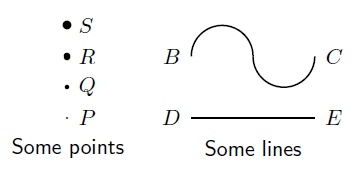
\includegraphics{col11306.imgs/m39370_MG10C13_001.png} % m39370;MG10C13\_001.png;;;6.0;8.5;
        
      \vspace{2pt}
    \vspace{\rubberspace}\par \begin{cnxcaption}
	  \small \textbf{Figure 12.1: }Examples of some points (labelled \begin{math}P\end{math}, \begin{math}Q\end{math}, \begin{math}R\end{math} and \begin{math}S\end{math}\hspace{1ex}) and some lines (labelled \begin{math}BC\end{math} and \begin{math}DE\end{math}\hspace{1ex}).
	\end{cnxcaption}
      
    \vspace{.1in}
    \rule[.1in]{\figurerulewidth}{.005in} \\
        
    \end{center}

 \end{figure}   

    \addtocounter{footnote}{-0}
    
      \label{m39370*id313170}Lines are labelled according to the start point and end point. We call the line that starts at a point \begin{math}A\end{math} and ends at a point \begin{math}B\end{math}, \begin{math}AB\end{math}. Since the line from point \begin{math}B\end{math} to point \begin{math}A\end{math} is the same as the line from point \begin{math}A\end{math} to point \begin{math}B\end{math}, we have that \begin{math}AB=BA\end{math}.\par 
      \label{m39370*id313175}When there is no ambiguity (which is the case throughout this text) the length of the line between points \begin{math}A\end{math} and \begin{math}B\end{math} is also denoted \begin{math}AB\end{math}\hspace{1ex}, the same as the notation to refer to the line itself. So if we say \begin{math}AB=CD\end{math}\hspace{1ex} we mean that the length of the line between \begin{math}A\end{math} and \begin{math}B\end{math} is equal to the length of the line between \begin{math}C\end{math} and \begin{math}D\end{math}.

\par 
      \label{m39370*eip-313}Note: in higher mathematics, where there might be some ambiguity between when we want refer to the length of the line and when we just want to refer to the line itself, the notation \begin{math}|AB|\end{math}\hspace{1ex} is usually used to refer to the length of the line. In this case, if one says \begin{math}|AB|=|CD|\end{math}, it means the lengths of the lines are the same, whereas if one says \begin{math}AB=CD\end{math}, it means that the two lines actually coincide (i.e. they are the same). Throughout this text, however, this notation will not be used, and \begin{math}AB=CD\end{math} ALWAYS implies that the lengths are the same. \par \label{m39370*id314000}A line is measured in \textsl{units of length}. Some common units of length are listed in Table 12.1.\par 
      
    % \textbf{m39370*uid8}\par
    
    % how many colspecs?  2
          % name: cnx:colspec
            % colnum: 1
            % colwidth: 10*
            % latex-name: columna
            % colname: 
            % align/tgroup-align/default: //left
            % -------------------------
            % name: cnx:colspec
            % colnum: 2
            % colwidth: 10*
            % latex-name: columnb
            % colname: 
            % align/tgroup-align/default: //left
            % -------------------------
      
    
    \setlength\mytablespace{4\tabcolsep}
    \addtolength\mytablespace{3\arrayrulewidth}
    \setlength\mytablewidth{\linewidth}
        
    
    \setlength\mytableroom{\mytablewidth}
    \addtolength\mytableroom{-\mytablespace}
    
    \setlength\myfixedwidth{0pt}
    \setlength\mystarwidth{\mytableroom}
        \addtolength\mystarwidth{-\myfixedwidth}
        \divide\mystarwidth 20
        
    
      % ----- Begin capturing width of table in LR mode woof
      \settowidth{\mytableboxwidth}{\begin{tabular}[t]{|l|l|}\hline
    % count in rowspan-info-nodeset: 2
    % align/colidx: left,1
    
    % rowcount: '0' | start: 'false' | colidx: '1'
    
        % Formatting a regular cell and recurring on the next sibling
        
                \textbf{Unit of Length}
               &
      % align/colidx: left,2
    
    % rowcount: '0' | start: 'false' | colidx: '2'
    
        % Formatting a regular cell and recurring on the next sibling
        
                \textbf{Abbreviation}
              % make-rowspan-placeholders
    % rowspan info: col1 '0' | 'false' | '' || col2 '0' | 'false' | ''
     \tabularnewline\cline{1-1}\cline{2-2}
      %--------------------------------------------------------------------
    % align/colidx: left,1
    
    % rowcount: '0' | start: 'false' | colidx: '1'
    
        % Formatting a regular cell and recurring on the next sibling
        kilometre &
      % align/colidx: left,2
    
    % rowcount: '0' | start: 'false' | colidx: '2'
    
        % Formatting a regular cell and recurring on the next sibling
        km% make-rowspan-placeholders
    % rowspan info: col1 '0' | 'false' | '' || col2 '0' | 'false' | ''
     \tabularnewline\cline{1-1}\cline{2-2}
      %--------------------------------------------------------------------
    % align/colidx: left,1
    
    % rowcount: '0' | start: 'false' | colidx: '1'
    
        % Formatting a regular cell and recurring on the next sibling
        metre &
      % align/colidx: left,2
    
    % rowcount: '0' | start: 'false' | colidx: '2'
    
        % Formatting a regular cell and recurring on the next sibling
        m% make-rowspan-placeholders
    % rowspan info: col1 '0' | 'false' | '' || col2 '0' | 'false' | ''
     \tabularnewline\cline{1-1}\cline{2-2}
      %--------------------------------------------------------------------
    % align/colidx: left,1
    
    % rowcount: '0' | start: 'false' | colidx: '1'
    
        % Formatting a regular cell and recurring on the next sibling
        centimetre &
      % align/colidx: left,2
    
    % rowcount: '0' | start: 'false' | colidx: '2'
    
        % Formatting a regular cell and recurring on the next sibling
        cm% make-rowspan-placeholders
    % rowspan info: col1 '0' | 'false' | '' || col2 '0' | 'false' | ''
     \tabularnewline\cline{1-1}\cline{2-2}
      %--------------------------------------------------------------------
    % align/colidx: left,1
    
    % rowcount: '0' | start: 'false' | colidx: '1'
    
        % Formatting a regular cell and recurring on the next sibling
        millimetre &
      % align/colidx: left,2
    
    % rowcount: '0' | start: 'false' | colidx: '2'
    
        % Formatting a regular cell and recurring on the next sibling
        mm% make-rowspan-placeholders
    % rowspan info: col1 '0' | 'false' | '' || col2 '0' | 'false' | ''
     \tabularnewline\cline{1-1}\cline{2-2}
      %--------------------------------------------------------------------
    \end{tabular}} % end mytableboxwidth set
      \addtocounter{footnote}{-0}
      
      % ----- End capturing width of table in LR mode
    
        % ----- LR or paragraph mode: must test
        % ----- Begin capturing height of table
        \settoheight{\mytableboxheight}{\begin{tabular}[t]{|l|l|}\hline
    % count in rowspan-info-nodeset: 2
    % align/colidx: left,1
    
    % rowcount: '0' | start: 'false' | colidx: '1'
    
        % Formatting a regular cell and recurring on the next sibling
        
                \textbf{Unit of Length}
               &
      % align/colidx: left,2
    
    % rowcount: '0' | start: 'false' | colidx: '2'
    
        % Formatting a regular cell and recurring on the next sibling
        
                \textbf{Abbreviation}
              % make-rowspan-placeholders
    % rowspan info: col1 '0' | 'false' | '' || col2 '0' | 'false' | ''
     \tabularnewline\cline{1-1}\cline{2-2}
      %--------------------------------------------------------------------
    % align/colidx: left,1
    
    % rowcount: '0' | start: 'false' | colidx: '1'
    
        % Formatting a regular cell and recurring on the next sibling
        kilometre &
      % align/colidx: left,2
    
    % rowcount: '0' | start: 'false' | colidx: '2'
    
        % Formatting a regular cell and recurring on the next sibling
        km% make-rowspan-placeholders
    % rowspan info: col1 '0' | 'false' | '' || col2 '0' | 'false' | ''
     \tabularnewline\cline{1-1}\cline{2-2}
      %--------------------------------------------------------------------
    % align/colidx: left,1
    
    % rowcount: '0' | start: 'false' | colidx: '1'
    
        % Formatting a regular cell and recurring on the next sibling
        metre &
      % align/colidx: left,2
    
    % rowcount: '0' | start: 'false' | colidx: '2'
    
        % Formatting a regular cell and recurring on the next sibling
        m% make-rowspan-placeholders
    % rowspan info: col1 '0' | 'false' | '' || col2 '0' | 'false' | ''
     \tabularnewline\cline{1-1}\cline{2-2}
      %--------------------------------------------------------------------
    % align/colidx: left,1
    
    % rowcount: '0' | start: 'false' | colidx: '1'
    
        % Formatting a regular cell and recurring on the next sibling
        centimetre &
      % align/colidx: left,2
    
    % rowcount: '0' | start: 'false' | colidx: '2'
    
        % Formatting a regular cell and recurring on the next sibling
        cm% make-rowspan-placeholders
    % rowspan info: col1 '0' | 'false' | '' || col2 '0' | 'false' | ''
     \tabularnewline\cline{1-1}\cline{2-2}
      %--------------------------------------------------------------------
    % align/colidx: left,1
    
    % rowcount: '0' | start: 'false' | colidx: '1'
    
        % Formatting a regular cell and recurring on the next sibling
        millimetre &
      % align/colidx: left,2
    
    % rowcount: '0' | start: 'false' | colidx: '2'
    
        % Formatting a regular cell and recurring on the next sibling
        mm% make-rowspan-placeholders
    % rowspan info: col1 '0' | 'false' | '' || col2 '0' | 'false' | ''
     \tabularnewline\cline{1-1}\cline{2-2}
      %--------------------------------------------------------------------
    \end{tabular}} % end mytableboxheight set
        \settodepth{\mytableboxdepth}{\begin{tabular}[t]{|l|l|}\hline
    % count in rowspan-info-nodeset: 2
    % align/colidx: left,1
    
    % rowcount: '0' | start: 'false' | colidx: '1'
    
        % Formatting a regular cell and recurring on the next sibling
        
                \textbf{Unit of Length}
               &
      % align/colidx: left,2
    
    % rowcount: '0' | start: 'false' | colidx: '2'
    
        % Formatting a regular cell and recurring on the next sibling
        
                \textbf{Abbreviation}
              % make-rowspan-placeholders
    % rowspan info: col1 '0' | 'false' | '' || col2 '0' | 'false' | ''
     \tabularnewline\cline{1-1}\cline{2-2}
      %--------------------------------------------------------------------
    % align/colidx: left,1
    
    % rowcount: '0' | start: 'false' | colidx: '1'
    
        % Formatting a regular cell and recurring on the next sibling
        kilometre &
      % align/colidx: left,2
    
    % rowcount: '0' | start: 'false' | colidx: '2'
    
        % Formatting a regular cell and recurring on the next sibling
        km% make-rowspan-placeholders
    % rowspan info: col1 '0' | 'false' | '' || col2 '0' | 'false' | ''
     \tabularnewline\cline{1-1}\cline{2-2}
      %--------------------------------------------------------------------
    % align/colidx: left,1
    
    % rowcount: '0' | start: 'false' | colidx: '1'
    
        % Formatting a regular cell and recurring on the next sibling
        metre &
      % align/colidx: left,2
    
    % rowcount: '0' | start: 'false' | colidx: '2'
    
        % Formatting a regular cell and recurring on the next sibling
        m% make-rowspan-placeholders
    % rowspan info: col1 '0' | 'false' | '' || col2 '0' | 'false' | ''
     \tabularnewline\cline{1-1}\cline{2-2}
      %--------------------------------------------------------------------
    % align/colidx: left,1
    
    % rowcount: '0' | start: 'false' | colidx: '1'
    
        % Formatting a regular cell and recurring on the next sibling
        centimetre &
      % align/colidx: left,2
    
    % rowcount: '0' | start: 'false' | colidx: '2'
    
        % Formatting a regular cell and recurring on the next sibling
        cm% make-rowspan-placeholders
    % rowspan info: col1 '0' | 'false' | '' || col2 '0' | 'false' | ''
     \tabularnewline\cline{1-1}\cline{2-2}
      %--------------------------------------------------------------------
    % align/colidx: left,1
    
    % rowcount: '0' | start: 'false' | colidx: '1'
    
        % Formatting a regular cell and recurring on the next sibling
        millimetre &
      % align/colidx: left,2
    
    % rowcount: '0' | start: 'false' | colidx: '2'
    
        % Formatting a regular cell and recurring on the next sibling
        mm% make-rowspan-placeholders
    % rowspan info: col1 '0' | 'false' | '' || col2 '0' | 'false' | ''
     \tabularnewline\cline{1-1}\cline{2-2}
      %--------------------------------------------------------------------
    \end{tabular}} % end mytableboxdepth set
        \addtolength{\mytableboxheight}{\mytableboxdepth}
        % ----- End capturing height of table
        \addtocounter{footnote}{-0}
        
        \ifthenelse{\mytableboxwidth<\textwidth}{% the table fits in LR mode
          \addtolength{\mytableboxwidth}{-\mytablespace}
          \typeout{textheight: \the\textheight}
          \typeout{mytableboxheight: \the\mytableboxheight}
          \typeout{textwidth: \the\textwidth}
          \typeout{mytableboxwidth: \the\mytableboxwidth}
          \ifthenelse{\mytableboxheight<\textheight}{%
        
    % \begin{table}[H]
    % \\ '' '0'
    
        \begin{center}
      
      \label{m39370*uid8}
      
    \noindent
    \begin{tabular}[t]{|l|l|}\hline
    % count in rowspan-info-nodeset: 2
    % align/colidx: left,1
    
    % rowcount: '0' | start: 'false' | colidx: '1'
    
        % Formatting a regular cell and recurring on the next sibling
        
                \textbf{Unit of Length}
               &
      % align/colidx: left,2
    
    % rowcount: '0' | start: 'false' | colidx: '2'
    
        % Formatting a regular cell and recurring on the next sibling
        
                \textbf{Abbreviation}
              % make-rowspan-placeholders
    % rowspan info: col1 '0' | 'false' | '' || col2 '0' | 'false' | ''
     \tabularnewline\cline{1-1}\cline{2-2}
      %--------------------------------------------------------------------
    % align/colidx: left,1
    
    % rowcount: '0' | start: 'false' | colidx: '1'
    
        % Formatting a regular cell and recurring on the next sibling
        kilometre &
      % align/colidx: left,2
    
    % rowcount: '0' | start: 'false' | colidx: '2'
    
        % Formatting a regular cell and recurring on the next sibling
        km% make-rowspan-placeholders
    % rowspan info: col1 '0' | 'false' | '' || col2 '0' | 'false' | ''
     \tabularnewline\cline{1-1}\cline{2-2}
      %--------------------------------------------------------------------
    % align/colidx: left,1
    
    % rowcount: '0' | start: 'false' | colidx: '1'
    
        % Formatting a regular cell and recurring on the next sibling
        metre &
      % align/colidx: left,2
    
    % rowcount: '0' | start: 'false' | colidx: '2'
    
        % Formatting a regular cell and recurring on the next sibling
        m% make-rowspan-placeholders
    % rowspan info: col1 '0' | 'false' | '' || col2 '0' | 'false' | ''
     \tabularnewline\cline{1-1}\cline{2-2}
      %--------------------------------------------------------------------
    % align/colidx: left,1
    
    % rowcount: '0' | start: 'false' | colidx: '1'
    
        % Formatting a regular cell and recurring on the next sibling
        centimetre &
      % align/colidx: left,2
    
    % rowcount: '0' | start: 'false' | colidx: '2'
    
        % Formatting a regular cell and recurring on the next sibling
        cm% make-rowspan-placeholders
    % rowspan info: col1 '0' | 'false' | '' || col2 '0' | 'false' | ''
     \tabularnewline\cline{1-1}\cline{2-2}
      %--------------------------------------------------------------------
    % align/colidx: left,1
    
    % rowcount: '0' | start: 'false' | colidx: '1'
    
        % Formatting a regular cell and recurring on the next sibling
        millimetre &
      % align/colidx: left,2
    
    % rowcount: '0' | start: 'false' | colidx: '2'
    
        % Formatting a regular cell and recurring on the next sibling
        mm% make-rowspan-placeholders
    % rowspan info: col1 '0' | 'false' | '' || col2 '0' | 'false' | ''
     \tabularnewline\cline{1-1}\cline{2-2}
      %--------------------------------------------------------------------
    \end{tabular}
      \end{center}
    \begin{center}{\small\bfseries Table 12.1}: Some common units of length and their abbreviations.\end{center}
    %\end{table}
    
    \addtocounter{footnote}{-0}
    
          }{ % else
        
    % \begin{table}[H]
    % \\ '' '0'
    
        \begin{center}
      
      \label{m39370*uid8}
      
    \noindent
    \tabletail{%
        \hline
        \multicolumn{2}{|p{\mytableboxwidth}|}{\raggedleft \small \sl continued on next page}\\
        \hline
      }
      \tablelasttail{}
      \begin{xtabular}[t]{|l|l|}\hline
    % count in rowspan-info-nodeset: 2
    % align/colidx: left,1
    
    % rowcount: '0' | start: 'false' | colidx: '1'
    
        % Formatting a regular cell and recurring on the next sibling
        
                \textbf{Unit of Length}
               &
      % align/colidx: left,2
    
    % rowcount: '0' | start: 'false' | colidx: '2'
    
        % Formatting a regular cell and recurring on the next sibling
        
                \textbf{Abbreviation}
              % make-rowspan-placeholders
    % rowspan info: col1 '0' | 'false' | '' || col2 '0' | 'false' | ''
     \tabularnewline\cline{1-1}\cline{2-2}
      %--------------------------------------------------------------------
    % align/colidx: left,1
    
    % rowcount: '0' | start: 'false' | colidx: '1'
    
        % Formatting a regular cell and recurring on the next sibling
        kilometre &
      % align/colidx: left,2
    
    % rowcount: '0' | start: 'false' | colidx: '2'
    
        % Formatting a regular cell and recurring on the next sibling
        km% make-rowspan-placeholders
    % rowspan info: col1 '0' | 'false' | '' || col2 '0' | 'false' | ''
     \tabularnewline\cline{1-1}\cline{2-2}
      %--------------------------------------------------------------------
    % align/colidx: left,1
    
    % rowcount: '0' | start: 'false' | colidx: '1'
    
        % Formatting a regular cell and recurring on the next sibling
        metre &
      % align/colidx: left,2
    
    % rowcount: '0' | start: 'false' | colidx: '2'
    
        % Formatting a regular cell and recurring on the next sibling
        m% make-rowspan-placeholders
    % rowspan info: col1 '0' | 'false' | '' || col2 '0' | 'false' | ''
     \tabularnewline\cline{1-1}\cline{2-2}
      %--------------------------------------------------------------------
    % align/colidx: left,1
    
    % rowcount: '0' | start: 'false' | colidx: '1'
    
        % Formatting a regular cell and recurring on the next sibling
        centimetre &
      % align/colidx: left,2
    
    % rowcount: '0' | start: 'false' | colidx: '2'
    
        % Formatting a regular cell and recurring on the next sibling
        cm% make-rowspan-placeholders
    % rowspan info: col1 '0' | 'false' | '' || col2 '0' | 'false' | ''
     \tabularnewline\cline{1-1}\cline{2-2}
      %--------------------------------------------------------------------
    % align/colidx: left,1
    
    % rowcount: '0' | start: 'false' | colidx: '1'
    
        % Formatting a regular cell and recurring on the next sibling
        millimetre &
      % align/colidx: left,2
    
    % rowcount: '0' | start: 'false' | colidx: '2'
    
        % Formatting a regular cell and recurring on the next sibling
        mm% make-rowspan-placeholders
    % rowspan info: col1 '0' | 'false' | '' || col2 '0' | 'false' | ''
     \tabularnewline\cline{1-1}\cline{2-2}
      %--------------------------------------------------------------------
    \end{xtabular}
      \end{center}
    \begin{center}{\small\bfseries Table 12.1}: Some common units of length and their abbreviations.\end{center}
    %\end{table}
    
    \addtocounter{footnote}{-0}
    
          } % 
        }{% else
        % typeset the table in paragraph mode
        % ----- Begin capturing height of table
        \settoheight{\mytableboxheight}{\begin{tabular*}{\mytablewidth}[t]{|p{10\mystarwidth}|p{10\mystarwidth}|}\hline
    % count in rowspan-info-nodeset: 2
    % align/colidx: left,1
    
    % rowcount: '0' | start: 'false' | colidx: '1'
    
        % Formatting a regular cell and recurring on the next sibling
        
                \textbf{Unit of Length}
               &
      % align/colidx: left,2
    
    % rowcount: '0' | start: 'false' | colidx: '2'
    
        % Formatting a regular cell and recurring on the next sibling
        
                \textbf{Abbreviation}
              % make-rowspan-placeholders
    % rowspan info: col1 '0' | 'false' | '' || col2 '0' | 'false' | ''
     \tabularnewline\cline{1-1}\cline{2-2}
      %--------------------------------------------------------------------
    % align/colidx: left,1
    
    % rowcount: '0' | start: 'false' | colidx: '1'
    
        % Formatting a regular cell and recurring on the next sibling
        kilometre &
      % align/colidx: left,2
    
    % rowcount: '0' | start: 'false' | colidx: '2'
    
        % Formatting a regular cell and recurring on the next sibling
        km% make-rowspan-placeholders
    % rowspan info: col1 '0' | 'false' | '' || col2 '0' | 'false' | ''
     \tabularnewline\cline{1-1}\cline{2-2}
      %--------------------------------------------------------------------
    % align/colidx: left,1
    
    % rowcount: '0' | start: 'false' | colidx: '1'
    
        % Formatting a regular cell and recurring on the next sibling
        metre &
      % align/colidx: left,2
    
    % rowcount: '0' | start: 'false' | colidx: '2'
    
        % Formatting a regular cell and recurring on the next sibling
        m% make-rowspan-placeholders
    % rowspan info: col1 '0' | 'false' | '' || col2 '0' | 'false' | ''
     \tabularnewline\cline{1-1}\cline{2-2}
      %--------------------------------------------------------------------
    % align/colidx: left,1
    
    % rowcount: '0' | start: 'false' | colidx: '1'
    
        % Formatting a regular cell and recurring on the next sibling
        centimetre &
      % align/colidx: left,2
    
    % rowcount: '0' | start: 'false' | colidx: '2'
    
        % Formatting a regular cell and recurring on the next sibling
        cm% make-rowspan-placeholders
    % rowspan info: col1 '0' | 'false' | '' || col2 '0' | 'false' | ''
     \tabularnewline\cline{1-1}\cline{2-2}
      %--------------------------------------------------------------------
    % align/colidx: left,1
    
    % rowcount: '0' | start: 'false' | colidx: '1'
    
        % Formatting a regular cell and recurring on the next sibling
        millimetre &
      % align/colidx: left,2
    
    % rowcount: '0' | start: 'false' | colidx: '2'
    
        % Formatting a regular cell and recurring on the next sibling
        mm% make-rowspan-placeholders
    % rowspan info: col1 '0' | 'false' | '' || col2 '0' | 'false' | ''
     \tabularnewline\cline{1-1}\cline{2-2}
      %--------------------------------------------------------------------
    \end{tabular*}} % end mytableboxheight set
        \settodepth{\mytableboxdepth}{\begin{tabular*}{\mytablewidth}[t]{|p{10\mystarwidth}|p{10\mystarwidth}|}\hline
    % count in rowspan-info-nodeset: 2
    % align/colidx: left,1
    
    % rowcount: '0' | start: 'false' | colidx: '1'
    
        % Formatting a regular cell and recurring on the next sibling
        
                \textbf{Unit of Length}
               &
      % align/colidx: left,2
    
    % rowcount: '0' | start: 'false' | colidx: '2'
    
        % Formatting a regular cell and recurring on the next sibling
        
                \textbf{Abbreviation}
              % make-rowspan-placeholders
    % rowspan info: col1 '0' | 'false' | '' || col2 '0' | 'false' | ''
     \tabularnewline\cline{1-1}\cline{2-2}
      %--------------------------------------------------------------------
    % align/colidx: left,1
    
    % rowcount: '0' | start: 'false' | colidx: '1'
    
        % Formatting a regular cell and recurring on the next sibling
        kilometre &
      % align/colidx: left,2
    
    % rowcount: '0' | start: 'false' | colidx: '2'
    
        % Formatting a regular cell and recurring on the next sibling
        km% make-rowspan-placeholders
    % rowspan info: col1 '0' | 'false' | '' || col2 '0' | 'false' | ''
     \tabularnewline\cline{1-1}\cline{2-2}
      %--------------------------------------------------------------------
    % align/colidx: left,1
    
    % rowcount: '0' | start: 'false' | colidx: '1'
    
        % Formatting a regular cell and recurring on the next sibling
        metre &
      % align/colidx: left,2
    
    % rowcount: '0' | start: 'false' | colidx: '2'
    
        % Formatting a regular cell and recurring on the next sibling
        m% make-rowspan-placeholders
    % rowspan info: col1 '0' | 'false' | '' || col2 '0' | 'false' | ''
     \tabularnewline\cline{1-1}\cline{2-2}
      %--------------------------------------------------------------------
    % align/colidx: left,1
    
    % rowcount: '0' | start: 'false' | colidx: '1'
    
        % Formatting a regular cell and recurring on the next sibling
        centimetre &
      % align/colidx: left,2
    
    % rowcount: '0' | start: 'false' | colidx: '2'
    
        % Formatting a regular cell and recurring on the next sibling
        cm% make-rowspan-placeholders
    % rowspan info: col1 '0' | 'false' | '' || col2 '0' | 'false' | ''
     \tabularnewline\cline{1-1}\cline{2-2}
      %--------------------------------------------------------------------
    % align/colidx: left,1
    
    % rowcount: '0' | start: 'false' | colidx: '1'
    
        % Formatting a regular cell and recurring on the next sibling
        millimetre &
      % align/colidx: left,2
    
    % rowcount: '0' | start: 'false' | colidx: '2'
    
        % Formatting a regular cell and recurring on the next sibling
        mm% make-rowspan-placeholders
    % rowspan info: col1 '0' | 'false' | '' || col2 '0' | 'false' | ''
     \tabularnewline\cline{1-1}\cline{2-2}
      %--------------------------------------------------------------------
    \end{tabular*}} % end mytableboxdepth set
        \addtolength{\mytableboxheight}{\mytableboxdepth}
        % ----- End capturing height of table
        \typeout{textheight: \the\textheight}
        \typeout{mytableboxheight: \the\mytableboxheight}
        \typeout{table too wide, outputting in para mode}
        
    % \begin{table}[H]
    % \\ '' '0'
    
        \begin{center}
      
      \label{m39370*uid8}
      
    \noindent
    \tabletail{%
        \hline
        \multicolumn{2}{|p{\mytableroom}|}{\raggedleft \small \sl continued on next page}\\
        \hline
      }
      \tablelasttail{}
      \begin{xtabular*}{\mytablewidth}[t]{|p{10\mystarwidth}|p{10\mystarwidth}|}\hline
    % count in rowspan-info-nodeset: 2
    % align/colidx: left,1
    
    % rowcount: '0' | start: 'false' | colidx: '1'
    
        % Formatting a regular cell and recurring on the next sibling
        
                \textbf{Unit of Length}
               &
      % align/colidx: left,2
    
    % rowcount: '0' | start: 'false' | colidx: '2'
    
        % Formatting a regular cell and recurring on the next sibling
        
                \textbf{Abbreviation}
              % make-rowspan-placeholders
    % rowspan info: col1 '0' | 'false' | '' || col2 '0' | 'false' | ''
     \tabularnewline\cline{1-1}\cline{2-2}
      %--------------------------------------------------------------------
    % align/colidx: left,1
    
    % rowcount: '0' | start: 'false' | colidx: '1'
    
        % Formatting a regular cell and recurring on the next sibling
        kilometre &
      % align/colidx: left,2
    
    % rowcount: '0' | start: 'false' | colidx: '2'
    
        % Formatting a regular cell and recurring on the next sibling
        km% make-rowspan-placeholders
    % rowspan info: col1 '0' | 'false' | '' || col2 '0' | 'false' | ''
     \tabularnewline\cline{1-1}\cline{2-2}
      %--------------------------------------------------------------------
    % align/colidx: left,1
    
    % rowcount: '0' | start: 'false' | colidx: '1'
    
        % Formatting a regular cell and recurring on the next sibling
        metre &
      % align/colidx: left,2
    
    % rowcount: '0' | start: 'false' | colidx: '2'
    
        % Formatting a regular cell and recurring on the next sibling
        m% make-rowspan-placeholders
    % rowspan info: col1 '0' | 'false' | '' || col2 '0' | 'false' | ''
     \tabularnewline\cline{1-1}\cline{2-2}
      %--------------------------------------------------------------------
    % align/colidx: left,1
    
    % rowcount: '0' | start: 'false' | colidx: '1'
    
        % Formatting a regular cell and recurring on the next sibling
        centimetre &
      % align/colidx: left,2
    
    % rowcount: '0' | start: 'false' | colidx: '2'
    
        % Formatting a regular cell and recurring on the next sibling
        cm% make-rowspan-placeholders
    % rowspan info: col1 '0' | 'false' | '' || col2 '0' | 'false' | ''
     \tabularnewline\cline{1-1}\cline{2-2}
      %--------------------------------------------------------------------
    % align/colidx: left,1
    
    % rowcount: '0' | start: 'false' | colidx: '1'
    
        % Formatting a regular cell and recurring on the next sibling
        millimetre &
      % align/colidx: left,2
    
    % rowcount: '0' | start: 'false' | colidx: '2'
    
        % Formatting a regular cell and recurring on the next sibling
        mm% make-rowspan-placeholders
    % rowspan info: col1 '0' | 'false' | '' || col2 '0' | 'false' | ''
     \tabularnewline\cline{1-1}\cline{2-2}
      %--------------------------------------------------------------------
    \end{xtabular*}
      \end{center}
    \begin{center}{\small\bfseries Table 12.1}: Some common units of length and their abbreviations.\end{center}
    %\end{table}
    
    \addtocounter{footnote}{-0}
    
        }% ending lr/para test clause
      
    \par
  
    
    \label{m39370*cid4}
            \subsection{ Angles}
            \nopagebreak
            
      
      \label{m39370*id314141}An \textsl{angle} is formed when two straight lines meet at a point. The point at which two lines meet is known as a \textsl{vertex}. Angles are labelled with a \begin{math}\phantom{\rule{0.277778em}{0ex}}\hat{}\phantom{\rule{0.277778em}{0ex}}\end{math} called a caret on a letter. For example, in Figure~12.2 the angle is at \begin{math}\hat{B}\end{math}. Angles can also be labelled according to the line segments that make up the angle. For example, in Figure~12.2 the angle is made up when line segments \begin{math}CB\end{math} and \begin{math}BA\end{math} meet. So, the angle can be referred to as \begin{math}\angle CBA\end{math}\hspace{1ex} or \begin{math}\angle ABC\end{math}\hspace{1ex} or, if there is no ambiguity (i.e. there is only one angle at \begin{math}B\end{math}) sometimes simply \begin{math}\angle B\end{math}. The \begin{math}\angle \end{math} symbol is a short method of writing angle in geometry.\par 
      \label{m39370*id314241}Angles are measured in \textsl{degrees} which is denoted by \begin{math}{}^{\circ }\end{math}, a small circle raised above the text in the same fashion as an exponent (or a superscript).\par 
      \label{m39370*eip-522}\label{m39370*notfhsst!!!underscore!!!id43812}
\begin{tabular}{cc}
	\hspace*{-50pt}\raisebox{-8 mm}{\hspace{-0.2in}
\includegraphics[width=0.75in]{col11306.imgs/psfact2.png} } & 

	\begin{minipage}{0.85\textwidth}
	\begin{note}
      {note: }
        \label{m39370*id316245335}Angles can also be measured in radians. At high school level you will only use degrees, but if you decide to take maths at university you will learn about radians.
        \par 
	\end{note}
	\end{minipage}
	\end{tabular}
	\par
      \par 
    \setcounter{subfigure}{0}


	\begin{figure}[H] % horizontal\label{m39370*uid9}
    \begin{center}
    \rule[.1in]{\figurerulewidth}{.005in} \\
        \label{m39370*uid9!!!underscore!!!media}\label{m39370*uid9!!!underscore!!!printimage}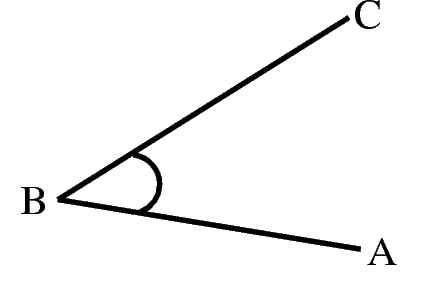
\includegraphics{col11306.imgs/m39370_MG10C13_002.png} % m39370;MG10C13\_002.png;;;6.0;8.5;
        
      \vspace{2pt}
    \vspace{\rubberspace}\par \begin{cnxcaption}
	  \small \textbf{Figure 12.2: }Angle labelled as \begin{math}\hat{B}\end{math}, \begin{math}\angle CBA\end{math}\hspace{1ex} or \begin{math}\angle ABC\end{math}
	\end{cnxcaption}
      
    \vspace{.1in}
    \rule[.1in]{\figurerulewidth}{.005in} \\
        
    \end{center}

 \end{figure}   

    \addtocounter{footnote}{-0}
    
      
    \setcounter{subfigure}{0}


	\begin{figure}[H] % horizontal\label{m39370*uid10}
    \begin{center}
    \rule[.1in]{\figurerulewidth}{.005in} \\
        \label{m39370*uid10!!!underscore!!!media}\label{m39370*uid10!!!underscore!!!printimage}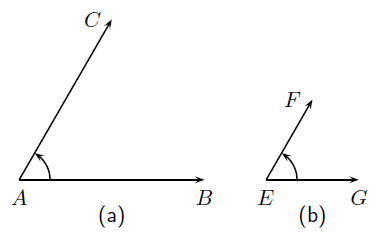
\includegraphics{col11306.imgs/m39370_MG10C13_003.png} % m39370;MG10C13\_003.png;;;6.0;8.5;
        
      \vspace{2pt}
    \vspace{\rubberspace}\par \begin{cnxcaption}
	  \small \textbf{Figure 12.3: }Examples of angles. \begin{math}\hat{A}=\hat{E}\end{math}, even though the lines making up the angles are of different lengths.
	\end{cnxcaption}
      
    \vspace{.1in}
    \rule[.1in]{\figurerulewidth}{.005in} \\
        
    \end{center}

 \end{figure}   

    \addtocounter{footnote}{-0}
    
      \label{m39370*uid11}
            \subsubsection{ Measuring angles}
            \nopagebreak
            
        
        \label{m39370*id314363}The size of an angle does not depend on the length of the lines that are joined to make up the angle, but depends only on how both the lines are placed as can be seen in Figure~12.3. This means that the idea of length cannot be used to measure angles. An angle is a rotation around the vertex.\par 
        \label{m39370*uid12}
            \subsubsection{ Using a Protractor}
            \nopagebreak
            
          
          \label{m39370*id314383}A protractor is a simple tool that is used to measure angles. A picture of a protractor is shown in Figure~12.4.\par 
          
    \setcounter{subfigure}{0}


	\begin{figure}[H] % horizontal\label{m39370*uid13}
    \begin{center}
    \rule[.1in]{\figurerulewidth}{.005in} \\
        \label{m39370*uid13!!!underscore!!!media}\label{m39370*uid13!!!underscore!!!printimage}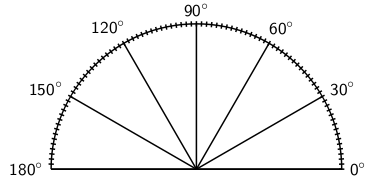
\includegraphics{col11306.imgs/m39370_MG10C13_004.png} % m39370;MG10C13\_004.png;;;6.0;8.5;
        
      \vspace{2pt}
    \vspace{\rubberspace}\par \begin{cnxcaption}
	  \small \textbf{Figure 12.4: }Diagram of a protractor.
	\end{cnxcaption}
      
    \vspace{.1in}
    \rule[.1in]{\figurerulewidth}{.005in} \\
        
    \end{center}

 \end{figure}   

    \addtocounter{footnote}{-0}
    
          \label{m39370*id314404}
            \textbf{Method:}
          \par 
          \label{m39370*id314412}Using a protractor\par 
          \label{m39370*id314417}\begin{enumerate}[noitemsep, label=\textbf{\arabic*}. ] 
            \label{m39370*uid14}\item Place the bottom line of the protractor along one line of the angle so that the other line of the angle points at the degree markings.
\label{m39370*uid15}\item Move the protractor along the line so that the centre point on the protractor is at the vertex of the two lines that make up the angle.
\label{m39370*uid16}\item Follow the second line until it meets the marking on the protractor and read off the angle. Make sure you start measuring at 0\begin{math}{}^{\circ }\end{math}.
\end{enumerate}
        
\label{m39370*secfhsst!!!underscore!!!id175}
            \subsubsection{  Measuring Angles : Use a protractor to measure the following angles:}
            \nopagebreak
            
          \label{m39370*id314481}
            
    \setcounter{subfigure}{0}


	\begin{figure}[H] % horizontal\label{m39370*id314484}
    \begin{center}
    \label{m39370*id314484!!!underscore!!!media}\label{m39370*id314484!!!underscore!!!printimage}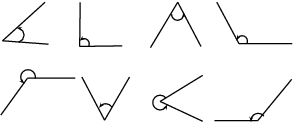
\includegraphics{col11306.imgs/m39370_MG10C13_005.png} % m39370;MG10C13\_005.png;;;6.0;8.5;
        
      \vspace{2pt}
    \vspace{.1in}
    
    \end{center}

 \end{figure}   

    \addtocounter{footnote}{-0}
    
          \par 
          
          

        
      
      \label{m39370*uid17}
            \subsubsection{ Special Angles}
            \nopagebreak
            
        
        \label{m39370*id314513}What is the smallest angle that can be drawn? The figure below shows two lines (\begin{math}CA\end{math} and \begin{math}AB\end{math}) making an angle at a common vertex \begin{math}A\end{math}. If line \begin{math}CA\end{math} is rotated around the common vertex \begin{math}A\end{math}, down towards line \begin{math}AB\end{math}, then the smallest angle that can be drawn occurs when the two lines are pointing in the same direction. This gives an angle of 0\begin{math}{}^{\circ }\end{math}. This is shown in Figure~12.6\par 
        \label{m39370*id314590}
    \setcounter{subfigure}{0}


	\begin{figure}[H] % horizontal\label{m39370*id314593}
    \begin{center}
    \label{m39370*id314593!!!underscore!!!media}\label{m39370*id314593!!!underscore!!!printimage}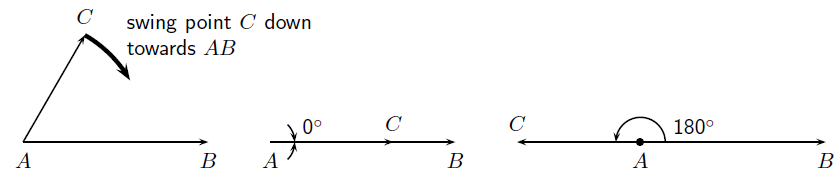
\includegraphics{col11306.imgs/m39370_MG10C13_006.png} % m39370;MG10C13\_006.png;;;6.0;8.5;
        
      \vspace{2pt}
    \vspace{.1in}
    
    \end{center}

 \end{figure}   

    \addtocounter{footnote}{-0}
    
        \par 
        \label{m39370*id314599}If line \begin{math}CA\end{math} is now swung upwards, any other angle can be obtained. If line \begin{math}CA\end{math} and line \begin{math}AB\end{math} point in opposite directions (the third case in Figure~12.6) then this forms an angle of 180\begin{math}{}^{\circ }\end{math}.\par 
\label{m39370*notfhsst!!!underscore!!!id201}
\begin{tabular}{cc}
	   \hspace*{-50pt}\raisebox{-8 mm}{ 
\includegraphics[width=0.5in]{col11306.imgs/pstip2.png}  }& 

	\begin{minipage}{0.85\textwidth}
	\begin{note}
      {tip: }If three points \begin{math}A\end{math}, \begin{math}B\end{math} and \begin{math}C\end{math} lie on a straight line, then the angle between them is 180\begin{math}{}^{\circ }\end{math}. Conversely, if the angle between three points is 180\begin{math}{}^{\circ }\end{math}, then the points lie on a straight line.
	\end{note}
	\end{minipage}
	\end{tabular}
	\par
      
        \label{m39370*id314704}An angle of 90\begin{math}{}^{\circ }\end{math} is called a \textsl{right angle}. A right angle is half the size of the angle made by a straight line (180\begin{math}{}^{\circ }\end{math}). We say \begin{math}CA\end{math} is \textsl{perpendicular} to \begin{math}AB\end{math} or \begin{math}CA\perp AB\end{math}\hspace{1ex}. An angle twice the size of a straight line is 360\begin{math}{}^{\circ }\end{math}. An angle measuring 360\begin{math}{}^{\circ }\end{math} looks identical to an angle of 0\begin{math}{}^{\circ }\end{math}, except for the labelling. We call this a \textsl{revolution}.\par 
        
    \setcounter{subfigure}{0}


	\begin{figure}[H] % horizontal\label{m39370*uid18}
    \begin{center}
    \rule[.1in]{\figurerulewidth}{.005in} \\
        \label{m39370*uid18!!!underscore!!!media}\label{m39370*uid18!!!underscore!!!printimage}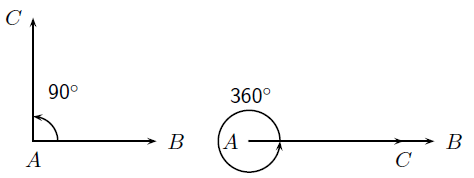
\includegraphics{col11306.imgs/m39370_MG10C13_007.png} % m39370;MG10C13\_007.png;;;6.0;8.5;
        
      \vspace{2pt}
    \vspace{\rubberspace}\par \begin{cnxcaption}
	  \small \textbf{Figure 12.7: }An angle of 90\begin{math}{}^{\circ }\end{math} is known as a \textsl{right angle}.
	\end{cnxcaption}
      
    \vspace{.1in}
    \rule[.1in]{\figurerulewidth}{.005in} \\
        
    \end{center}

 \end{figure}   

    \addtocounter{footnote}{-0}
    
\label{m39370*secfhsst!!!underscore!!!id210}
            \subsubsection{  Angles larger than 360${}^{\circ }$ }
            \nopagebreak
            
        \label{m39370*id314877}All angles larger than 360\begin{math}{}^{\circ }\end{math} also look like we have seen them before. If you are given an angle that is larger than 360\begin{math}{}^{\circ }\end{math}, continue subtracting 360\begin{math}{}^{\circ }\end{math} from the angle, until you get an answer that is between 0\begin{math}{}^{\circ }\end{math}and 360\begin{math}{}^{\circ }\end{math}. Angles that measure more than 360\begin{math}{}^{\circ }\end{math} are largely for mathematical convenience. \par 

\label{m39370*notfhsst!!!underscore!!!id213}
\begin{tabular}{cc}
	   \hspace*{-50pt}\raisebox{-8 mm}{ 
\includegraphics[width=0.5in]{col11306.imgs/pstip2.png}  }& 

	\begin{minipage}{0.85\textwidth}
	\begin{note}
      {tip: }
        \label{m39370*id314971}\begin{itemize}[noitemsep]
            \label{m39370*uid19}\item \textsl{Acute angle}: An angle \begin{math}\ge {0}^{\circ }\end{math} and \begin{math}\lessthan{}{90}^{\circ }\end{math}.
\label{m39370*uid20}\item \textsl{Right angle}: An angle measuring \begin{math}{90}^{\circ }\end{math}.
\label{m39370*uid21}\item \textsl{Obtuse angle}: An angle \begin{math}\greatthan{}{90}^{\circ }\end{math} and \begin{math}\lessthan{}{180}^{\circ }\end{math}.
\label{m39370*uid22}\item \textsl{Straight angle}: An angle measuring 180\begin{math}{}^{\circ }\end{math}.
\label{m39370*uid23}\item \textsl{Reflex angle}: An angle \begin{math}\greatthan{}{180}^{\circ }\end{math} and \begin{math}\lessthan{}{360}^{\circ }\end{math}.
\label{m39370*uid24}\item \textsl{Revolution}: An angle measuring \begin{math}{360}^{\circ }\end{math}.
\end{itemize}
        
        \label{m39370*id315224}These are simply labels for angles in particular ranges, shown in Figure~12.8.\par 
	\end{note}
	\end{minipage}
	\end{tabular}
	\par
      
        
    \setcounter{subfigure}{0}


	\begin{figure}[H] % horizontal\label{m39370*uid25}
    \begin{center}
    \rule[.1in]{\figurerulewidth}{.005in} \\
        \label{m39370*uid25!!!underscore!!!media}\label{m39370*uid25!!!underscore!!!printimage}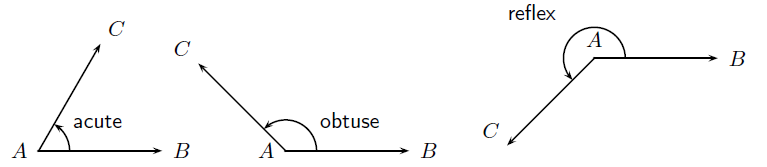
\includegraphics{col11306.imgs/m39370_MG10C13_008.png} % m39370;MG10C13\_008.png;;;6.0;8.5;
        
      \vspace{2pt}
    \vspace{\rubberspace}\par \begin{cnxcaption}
	  \small \textbf{Figure 12.8: }Three types of angles defined according to their ranges.
	\end{cnxcaption}
      
    \vspace{.1in}
    \rule[.1in]{\figurerulewidth}{.005in} \\
        
    \end{center}

 \end{figure}   

    \addtocounter{footnote}{-0}
    
        \label{m39370*id315245}Once angles can be measured, they can then be compared. For example, all right angles are 90\begin{math}{}^{\circ }\end{math}, therefore all right angles are equal and an obtuse angle will always be larger than an acute angle.\par \label{m39370*eip-752}The following video summarizes what you have learnt so far about angles.


    \setcounter{subfigure}{0}


	\begin{figure}[H] % horizontal\label{m39370*angles-1}
    
    
    \textnormal{Khan Academy video on angles - 1}\vspace{.1in} \nopagebreak
  \label{m39370*yt-media1}\label{m39370*yt-video1}
            \raisebox{-5 pt}{ 
\includegraphics[width=0.5cm]{col11306.imgs/summary_www.png}} { (Video:  MG10088 )}
      
      \vspace{2pt}
    \vspace{.1in}
    
    

 \end{figure}   

    \addtocounter{footnote}{-0}
    

Note that for high school trigonometry you will be using degrees, not radians as stated in the video. \par 
      
      \label{m39370*uid26}
            \subsubsection{ Special Angle Pairs}
            \nopagebreak
            
        
        \label{m39370*id315274}In Figure~12.10, straight lines \begin{math}AB\end{math} and \begin{math}CD\end{math} intersect at point X, forming four angles: \begin{math}\hat{{X}_{1}}\end{math} or \begin{math}\angle BXD\end{math}\hspace{1ex}, \begin{math}\hat{{X}_{2}}\end{math}\hspace{1ex} or \begin{math}\angle BXC\end{math}\hspace{1ex}, \begin{math}\hat{{X}_{3}}\end{math}\hspace{1ex} or \begin{math}\angle CXA\end{math}\hspace{1ex} and \begin{math}\hat{{X}_{4}}\end{math}\hspace{1ex} or \begin{math}\angle AXD\end{math}\hspace{1ex}.\par 
        
    \setcounter{subfigure}{0}


	\begin{figure}[H] % horizontal\label{m39370*uid27}
    \begin{center}
    \rule[.1in]{\figurerulewidth}{.005in} \\
        \label{m39370*uid27!!!underscore!!!media}\label{m39370*uid27!!!underscore!!!printimage}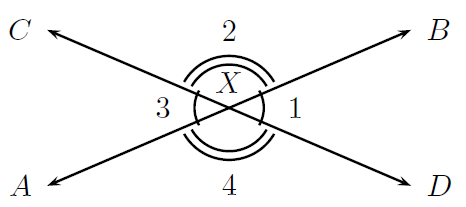
\includegraphics{col11306.imgs/m39370_MG10C13_009.png} % m39370;MG10C13\_009.png;;;6.0;8.5;
        
      \vspace{2pt}
    \vspace{\rubberspace}\par \begin{cnxcaption}
	  \small \textbf{Figure 12.10: }Two intersecting straight lines with vertical angles \begin{math}\hat{{X}_{1}},\hat{{X}_{3}}\end{math} and \begin{math}\hat{{X}_{2}},\hat{{X}_{4}}\end{math}.
	\end{cnxcaption}
      
    \vspace{.1in}
    \rule[.1in]{\figurerulewidth}{.005in} \\
        
    \end{center}

 \end{figure}   

    \addtocounter{footnote}{-0}
    
        \label{m39370*id315545}The table summarises the special angle pairs that result.\par 
        
    % \textbf{m39370*id315548}\par
    
    % how many colspecs?  3
          % name: cnx:colspec
            % colnum: 1
            % colwidth: 10*
            % latex-name: columna
            % colname: c1
            % align/tgroup-align/default: //left
            % -------------------------
            % name: cnx:colspec
            % colnum: 2
            % colwidth: 10*
            % latex-name: columnb
            % colname: c2
            % align/tgroup-align/default: //left
            % -------------------------
            % name: cnx:colspec
            % colnum: 3
            % colwidth: 10*
            % latex-name: columnc
            % colname: c3
            % align/tgroup-align/default: //left
            % -------------------------
      
    
    \setlength\mytablespace{6\tabcolsep}
    \addtolength\mytablespace{4\arrayrulewidth}
    \setlength\mytablewidth{\linewidth}
        
    
    \setlength\mytableroom{\mytablewidth}
    \addtolength\mytableroom{-\mytablespace}
    
    \setlength\myfixedwidth{0pt}
    \setlength\mystarwidth{\mytableroom}
        \addtolength\mystarwidth{-\myfixedwidth}
        \divide\mystarwidth 30
        
    
      % ----- Begin capturing width of table in LR mode woof
      \settowidth{\mytableboxwidth}{\begin{tabular}[t]{|l|l|l|}\hline
    % count in rowspan-info-nodeset: 3
    % align/colidx: left,1
    
    % rowcount: '0' | start: 'false' | colidx: '1'
    
        % Formatting a regular cell and recurring on the next sibling
        Special Angle &
      % align/colidx: left,2
    
    % rowcount: '0' | start: 'false' | colidx: '2'
    
        % Formatting a regular cell and recurring on the next sibling
        Property &
      % align/colidx: left,3
    
    % rowcount: '0' | start: 'false' | colidx: '3'
    
        % Formatting a regular cell and recurring on the next sibling
        Example% make-rowspan-placeholders
    % rowspan info: col1 '0' | 'false' | '' || col2 '0' | 'false' | '' || col3 '0' | 'false' | ''
     \tabularnewline\cline{1-1}\cline{2-2}\cline{3-3}
      %--------------------------------------------------------------------
    % align/colidx: left,1
    
    % rowcount: '0' | start: 'false' | colidx: '1'
    
        % Formatting a regular cell and recurring on the next sibling
        adjacent angles &
      % align/colidx: left,2
    
    % rowcount: '0' | start: 'false' | colidx: '2'
    
        % Formatting a regular cell and recurring on the next sibling
        share a common vertex and a common side &
      % align/colidx: left,3
    
    % rowcount: '0' | start: 'false' | colidx: '3'
    
        % Formatting a regular cell and recurring on the next sibling
        \begin{math}\left(\hat{{X}_{1}},\hat{{X}_{2}}\right)\end{math}, \begin{math}\left(\hat{{X}_{2}},\hat{{X}_{3}}\right)\end{math}, \begin{math}\left(\hat{{X}_{3}},\hat{{X}_{4}}\right)\end{math}, \begin{math}\left(\hat{{X}_{4}},\hat{{X}_{1}}\right)\end{math}% make-rowspan-placeholders
    % rowspan info: col1 '0' | 'false' | '' || col2 '0' | 'false' | '' || col3 '0' | 'false' | ''
     \tabularnewline\cline{1-1}\cline{2-2}\cline{3-3}
      %--------------------------------------------------------------------
    % align/colidx: left,1
    
    % rowcount: '0' | start: 'false' | colidx: '1'
    
        % Formatting a regular cell and recurring on the next sibling
        linear pair (adjacent angles on a straight line) &
      % align/colidx: left,2
    
    % rowcount: '0' | start: 'false' | colidx: '2'
    
        % Formatting a regular cell and recurring on the next sibling
        adjacent angles formed by two intersecting straight lines that by definition add to 180\begin{math}{}^{\circ }\end{math} &
      % align/colidx: left,3
    
    % rowcount: '0' | start: 'false' | colidx: '3'
    
        % Formatting a regular cell and recurring on the next sibling
        
                  \begin{math}\hat{{X}_{1}}+\hat{{X}_{2}}={180}^{\circ }\end{math};
                  \begin{math}\hat{{X}_{2}}+\hat{{X}_{3}}={180}^{\circ }\end{math};
                  \begin{math}\hat{{X}_{3}}+\hat{{X}_{4}}={180}^{\circ }\end{math};
                  \begin{math}\hat{{X}_{4}}+\hat{{X}_{1}}={180}^{\circ }\end{math}
                % make-rowspan-placeholders
    % rowspan info: col1 '0' | 'false' | '' || col2 '0' | 'false' | '' || col3 '0' | 'false' | ''
     \tabularnewline\cline{1-1}\cline{2-2}\cline{3-3}
      %--------------------------------------------------------------------
    % align/colidx: left,1
    
    % rowcount: '0' | start: 'false' | colidx: '1'
    
        % Formatting a regular cell and recurring on the next sibling
        opposite angles &
      % align/colidx: left,2
    
    % rowcount: '0' | start: 'false' | colidx: '2'
    
        % Formatting a regular cell and recurring on the next sibling
        angles formed by two intersecting straight lines that share a vertex but do not share any sides &
      % align/colidx: left,3
    
    % rowcount: '0' | start: 'false' | colidx: '3'
    
        % Formatting a regular cell and recurring on the next sibling
        
                  \begin{math}\hat{{X}_{1}}=\hat{{X}_{3}}\end{math};
                  \begin{math}\hat{{X}_{2}}=\hat{{X}_{4}}\end{math}
                % make-rowspan-placeholders
    % rowspan info: col1 '0' | 'false' | '' || col2 '0' | 'false' | '' || col3 '0' | 'false' | ''
     \tabularnewline\cline{1-1}\cline{2-2}\cline{3-3}
      %--------------------------------------------------------------------
    % align/colidx: left,1
    
    % rowcount: '0' | start: 'false' | colidx: '1'
    
        % Formatting a regular cell and recurring on the next sibling
        supplementary angles &
      % My position: 1
    % my spanname: 
    % my ct of spanspec: 0
    % my column-count: 2
    % align/colidx: center,2
    \multicolumn{2}{c|}{two angles whose sum is 180\begin{math}{}^{\circ }\end{math}}
    % rowspan info: col1 '0' | 'false' | '' || col2 '0' | 'false' | '' || col3 '0' | 'false' | ''
     \tabularnewline\cline{1-1}\cline{2-2}\cline{3-3}
      %--------------------------------------------------------------------
    % align/colidx: left,1
    
    % rowcount: '0' | start: 'false' | colidx: '1'
    
        % Formatting a regular cell and recurring on the next sibling
        complementary angles &
      % My position: 1
    % my spanname: 
    % my ct of spanspec: 0
    % my column-count: 2
    % align/colidx: center,2
    \multicolumn{2}{c|}{two angles whose sum is 90\begin{math}{}^{\circ }\end{math}}
    % rowspan info: col1 '0' | 'false' | '' || col2 '0' | 'false' | '' || col3 '0' | 'false' | ''
     \tabularnewline\cline{1-1}\cline{2-2}\cline{3-3}
      %--------------------------------------------------------------------
    \end{tabular}} % end mytableboxwidth set
      \addtocounter{footnote}{-0}
      
      % ----- End capturing width of table in LR mode
    
        % ----- LR or paragraph mode: must test
        % ----- Begin capturing height of table
        \settoheight{\mytableboxheight}{\begin{tabular}[t]{|l|l|l|}\hline
    % count in rowspan-info-nodeset: 3
    % align/colidx: left,1
    
    % rowcount: '0' | start: 'false' | colidx: '1'
    
        % Formatting a regular cell and recurring on the next sibling
        Special Angle &
      % align/colidx: left,2
    
    % rowcount: '0' | start: 'false' | colidx: '2'
    
        % Formatting a regular cell and recurring on the next sibling
        Property &
      % align/colidx: left,3
    
    % rowcount: '0' | start: 'false' | colidx: '3'
    
        % Formatting a regular cell and recurring on the next sibling
        Example% make-rowspan-placeholders
    % rowspan info: col1 '0' | 'false' | '' || col2 '0' | 'false' | '' || col3 '0' | 'false' | ''
     \tabularnewline\cline{1-1}\cline{2-2}\cline{3-3}
      %--------------------------------------------------------------------
    % align/colidx: left,1
    
    % rowcount: '0' | start: 'false' | colidx: '1'
    
        % Formatting a regular cell and recurring on the next sibling
        adjacent angles &
      % align/colidx: left,2
    
    % rowcount: '0' | start: 'false' | colidx: '2'
    
        % Formatting a regular cell and recurring on the next sibling
        share a common vertex and a common side &
      % align/colidx: left,3
    
    % rowcount: '0' | start: 'false' | colidx: '3'
    
        % Formatting a regular cell and recurring on the next sibling
        \begin{math}\left(\hat{{X}_{1}},\hat{{X}_{2}}\right)\end{math}, \begin{math}\left(\hat{{X}_{2}},\hat{{X}_{3}}\right)\end{math}, \begin{math}\left(\hat{{X}_{3}},\hat{{X}_{4}}\right)\end{math}, \begin{math}\left(\hat{{X}_{4}},\hat{{X}_{1}}\right)\end{math}% make-rowspan-placeholders
    % rowspan info: col1 '0' | 'false' | '' || col2 '0' | 'false' | '' || col3 '0' | 'false' | ''
     \tabularnewline\cline{1-1}\cline{2-2}\cline{3-3}
      %--------------------------------------------------------------------
    % align/colidx: left,1
    
    % rowcount: '0' | start: 'false' | colidx: '1'
    
        % Formatting a regular cell and recurring on the next sibling
        linear pair (adjacent angles on a straight line) &
      % align/colidx: left,2
    
    % rowcount: '0' | start: 'false' | colidx: '2'
    
        % Formatting a regular cell and recurring on the next sibling
        adjacent angles formed by two intersecting straight lines that by definition add to 180\begin{math}{}^{\circ }\end{math} &
      % align/colidx: left,3
    
    % rowcount: '0' | start: 'false' | colidx: '3'
    
        % Formatting a regular cell and recurring on the next sibling
        
                  \begin{math}\hat{{X}_{1}}+\hat{{X}_{2}}={180}^{\circ }\end{math};
                  \begin{math}\hat{{X}_{2}}+\hat{{X}_{3}}={180}^{\circ }\end{math};
                  \begin{math}\hat{{X}_{3}}+\hat{{X}_{4}}={180}^{\circ }\end{math};
                  \begin{math}\hat{{X}_{4}}+\hat{{X}_{1}}={180}^{\circ }\end{math}
                % make-rowspan-placeholders
    % rowspan info: col1 '0' | 'false' | '' || col2 '0' | 'false' | '' || col3 '0' | 'false' | ''
     \tabularnewline\cline{1-1}\cline{2-2}\cline{3-3}
      %--------------------------------------------------------------------
    % align/colidx: left,1
    
    % rowcount: '0' | start: 'false' | colidx: '1'
    
        % Formatting a regular cell and recurring on the next sibling
        opposite angles &
      % align/colidx: left,2
    
    % rowcount: '0' | start: 'false' | colidx: '2'
    
        % Formatting a regular cell and recurring on the next sibling
        angles formed by two intersecting straight lines that share a vertex but do not share any sides &
      % align/colidx: left,3
    
    % rowcount: '0' | start: 'false' | colidx: '3'
    
        % Formatting a regular cell and recurring on the next sibling
        
                  \begin{math}\hat{{X}_{1}}=\hat{{X}_{3}}\end{math};
                  \begin{math}\hat{{X}_{2}}=\hat{{X}_{4}}\end{math}
                % make-rowspan-placeholders
    % rowspan info: col1 '0' | 'false' | '' || col2 '0' | 'false' | '' || col3 '0' | 'false' | ''
     \tabularnewline\cline{1-1}\cline{2-2}\cline{3-3}
      %--------------------------------------------------------------------
    % align/colidx: left,1
    
    % rowcount: '0' | start: 'false' | colidx: '1'
    
        % Formatting a regular cell and recurring on the next sibling
        supplementary angles &
      % My position: 1
    % my spanname: 
    % my ct of spanspec: 0
    % my column-count: 2
    % align/colidx: center,2
    \multicolumn{2}{c|}{two angles whose sum is 180\begin{math}{}^{\circ }\end{math}}
    % rowspan info: col1 '0' | 'false' | '' || col2 '0' | 'false' | '' || col3 '0' | 'false' | ''
     \tabularnewline\cline{1-1}\cline{2-2}\cline{3-3}
      %--------------------------------------------------------------------
    % align/colidx: left,1
    
    % rowcount: '0' | start: 'false' | colidx: '1'
    
        % Formatting a regular cell and recurring on the next sibling
        complementary angles &
      % My position: 1
    % my spanname: 
    % my ct of spanspec: 0
    % my column-count: 2
    % align/colidx: center,2
    \multicolumn{2}{c|}{two angles whose sum is 90\begin{math}{}^{\circ }\end{math}}
    % rowspan info: col1 '0' | 'false' | '' || col2 '0' | 'false' | '' || col3 '0' | 'false' | ''
     \tabularnewline\cline{1-1}\cline{2-2}\cline{3-3}
      %--------------------------------------------------------------------
    \end{tabular}} % end mytableboxheight set
        \settodepth{\mytableboxdepth}{\begin{tabular}[t]{|l|l|l|}\hline
    % count in rowspan-info-nodeset: 3
    % align/colidx: left,1
    
    % rowcount: '0' | start: 'false' | colidx: '1'
    
        % Formatting a regular cell and recurring on the next sibling
        Special Angle &
      % align/colidx: left,2
    
    % rowcount: '0' | start: 'false' | colidx: '2'
    
        % Formatting a regular cell and recurring on the next sibling
        Property &
      % align/colidx: left,3
    
    % rowcount: '0' | start: 'false' | colidx: '3'
    
        % Formatting a regular cell and recurring on the next sibling
        Example% make-rowspan-placeholders
    % rowspan info: col1 '0' | 'false' | '' || col2 '0' | 'false' | '' || col3 '0' | 'false' | ''
     \tabularnewline\cline{1-1}\cline{2-2}\cline{3-3}
      %--------------------------------------------------------------------
    % align/colidx: left,1
    
    % rowcount: '0' | start: 'false' | colidx: '1'
    
        % Formatting a regular cell and recurring on the next sibling
        adjacent angles &
      % align/colidx: left,2
    
    % rowcount: '0' | start: 'false' | colidx: '2'
    
        % Formatting a regular cell and recurring on the next sibling
        share a common vertex and a common side &
      % align/colidx: left,3
    
    % rowcount: '0' | start: 'false' | colidx: '3'
    
        % Formatting a regular cell and recurring on the next sibling
        \begin{math}\left(\hat{{X}_{1}},\hat{{X}_{2}}\right)\end{math}, \begin{math}\left(\hat{{X}_{2}},\hat{{X}_{3}}\right)\end{math}, \begin{math}\left(\hat{{X}_{3}},\hat{{X}_{4}}\right)\end{math}, \begin{math}\left(\hat{{X}_{4}},\hat{{X}_{1}}\right)\end{math}% make-rowspan-placeholders
    % rowspan info: col1 '0' | 'false' | '' || col2 '0' | 'false' | '' || col3 '0' | 'false' | ''
     \tabularnewline\cline{1-1}\cline{2-2}\cline{3-3}
      %--------------------------------------------------------------------
    % align/colidx: left,1
    
    % rowcount: '0' | start: 'false' | colidx: '1'
    
        % Formatting a regular cell and recurring on the next sibling
        linear pair (adjacent angles on a straight line) &
      % align/colidx: left,2
    
    % rowcount: '0' | start: 'false' | colidx: '2'
    
        % Formatting a regular cell and recurring on the next sibling
        adjacent angles formed by two intersecting straight lines that by definition add to 180\begin{math}{}^{\circ }\end{math} &
      % align/colidx: left,3
    
    % rowcount: '0' | start: 'false' | colidx: '3'
    
        % Formatting a regular cell and recurring on the next sibling
        
                  \begin{math}\hat{{X}_{1}}+\hat{{X}_{2}}={180}^{\circ }\end{math};
                  \begin{math}\hat{{X}_{2}}+\hat{{X}_{3}}={180}^{\circ }\end{math};
                  \begin{math}\hat{{X}_{3}}+\hat{{X}_{4}}={180}^{\circ }\end{math};
                  \begin{math}\hat{{X}_{4}}+\hat{{X}_{1}}={180}^{\circ }\end{math}
                % make-rowspan-placeholders
    % rowspan info: col1 '0' | 'false' | '' || col2 '0' | 'false' | '' || col3 '0' | 'false' | ''
     \tabularnewline\cline{1-1}\cline{2-2}\cline{3-3}
      %--------------------------------------------------------------------
    % align/colidx: left,1
    
    % rowcount: '0' | start: 'false' | colidx: '1'
    
        % Formatting a regular cell and recurring on the next sibling
        opposite angles &
      % align/colidx: left,2
    
    % rowcount: '0' | start: 'false' | colidx: '2'
    
        % Formatting a regular cell and recurring on the next sibling
        angles formed by two intersecting straight lines that share a vertex but do not share any sides &
      % align/colidx: left,3
    
    % rowcount: '0' | start: 'false' | colidx: '3'
    
        % Formatting a regular cell and recurring on the next sibling
        
                  \begin{math}\hat{{X}_{1}}=\hat{{X}_{3}}\end{math};
                  \begin{math}\hat{{X}_{2}}=\hat{{X}_{4}}\end{math}
                % make-rowspan-placeholders
    % rowspan info: col1 '0' | 'false' | '' || col2 '0' | 'false' | '' || col3 '0' | 'false' | ''
     \tabularnewline\cline{1-1}\cline{2-2}\cline{3-3}
      %--------------------------------------------------------------------
    % align/colidx: left,1
    
    % rowcount: '0' | start: 'false' | colidx: '1'
    
        % Formatting a regular cell and recurring on the next sibling
        supplementary angles &
      % My position: 1
    % my spanname: 
    % my ct of spanspec: 0
    % my column-count: 2
    % align/colidx: center,2
    \multicolumn{2}{c|}{two angles whose sum is 180\begin{math}{}^{\circ }\end{math}}
    % rowspan info: col1 '0' | 'false' | '' || col2 '0' | 'false' | '' || col3 '0' | 'false' | ''
     \tabularnewline\cline{1-1}\cline{2-2}\cline{3-3}
      %--------------------------------------------------------------------
    % align/colidx: left,1
    
    % rowcount: '0' | start: 'false' | colidx: '1'
    
        % Formatting a regular cell and recurring on the next sibling
        complementary angles &
      % My position: 1
    % my spanname: 
    % my ct of spanspec: 0
    % my column-count: 2
    % align/colidx: center,2
    \multicolumn{2}{c|}{two angles whose sum is 90\begin{math}{}^{\circ }\end{math}}
    % rowspan info: col1 '0' | 'false' | '' || col2 '0' | 'false' | '' || col3 '0' | 'false' | ''
     \tabularnewline\cline{1-1}\cline{2-2}\cline{3-3}
      %--------------------------------------------------------------------
    \end{tabular}} % end mytableboxdepth set
        \addtolength{\mytableboxheight}{\mytableboxdepth}
        % ----- End capturing height of table
        \addtocounter{footnote}{-0}
        
        \ifthenelse{\mytableboxwidth<\textwidth}{% the table fits in LR mode
          \addtolength{\mytableboxwidth}{-\mytablespace}
          \typeout{textheight: \the\textheight}
          \typeout{mytableboxheight: \the\mytableboxheight}
          \typeout{textwidth: \the\textwidth}
          \typeout{mytableboxwidth: \the\mytableboxwidth}
          \ifthenelse{\mytableboxheight<\textheight}{%
        
    % \begin{table}[H]
    % \\ '' '0'
    
        \begin{center}
      
      \label{m39370*id315548}
      
    \noindent
    \begin{tabular}[t]{|l|l|l|}\hline
    % count in rowspan-info-nodeset: 3
    % align/colidx: left,1
    
    % rowcount: '0' | start: 'false' | colidx: '1'
    
        % Formatting a regular cell and recurring on the next sibling
        Special Angle &
      % align/colidx: left,2
    
    % rowcount: '0' | start: 'false' | colidx: '2'
    
        % Formatting a regular cell and recurring on the next sibling
        Property &
      % align/colidx: left,3
    
    % rowcount: '0' | start: 'false' | colidx: '3'
    
        % Formatting a regular cell and recurring on the next sibling
        Example% make-rowspan-placeholders
    % rowspan info: col1 '0' | 'false' | '' || col2 '0' | 'false' | '' || col3 '0' | 'false' | ''
     \tabularnewline\cline{1-1}\cline{2-2}\cline{3-3}
      %--------------------------------------------------------------------
    % align/colidx: left,1
    
    % rowcount: '0' | start: 'false' | colidx: '1'
    
        % Formatting a regular cell and recurring on the next sibling
        adjacent angles &
      % align/colidx: left,2
    
    % rowcount: '0' | start: 'false' | colidx: '2'
    
        % Formatting a regular cell and recurring on the next sibling
        share a common vertex and a common side &
      % align/colidx: left,3
    
    % rowcount: '0' | start: 'false' | colidx: '3'
    
        % Formatting a regular cell and recurring on the next sibling
        \begin{math}\left(\hat{{X}_{1}},\hat{{X}_{2}}\right)\end{math}, \begin{math}\left(\hat{{X}_{2}},\hat{{X}_{3}}\right)\end{math}, \begin{math}\left(\hat{{X}_{3}},\hat{{X}_{4}}\right)\end{math}, \begin{math}\left(\hat{{X}_{4}},\hat{{X}_{1}}\right)\end{math}% make-rowspan-placeholders
    % rowspan info: col1 '0' | 'false' | '' || col2 '0' | 'false' | '' || col3 '0' | 'false' | ''
     \tabularnewline\cline{1-1}\cline{2-2}\cline{3-3}
      %--------------------------------------------------------------------
    % align/colidx: left,1
    
    % rowcount: '0' | start: 'false' | colidx: '1'
    
        % Formatting a regular cell and recurring on the next sibling
        linear pair (adjacent angles on a straight line) &
      % align/colidx: left,2
    
    % rowcount: '0' | start: 'false' | colidx: '2'
    
        % Formatting a regular cell and recurring on the next sibling
        adjacent angles formed by two intersecting straight lines that by definition add to 180\begin{math}{}^{\circ }\end{math} &
      % align/colidx: left,3
    
    % rowcount: '0' | start: 'false' | colidx: '3'
    
        % Formatting a regular cell and recurring on the next sibling
        
                  \begin{math}\hat{{X}_{1}}+\hat{{X}_{2}}={180}^{\circ }\end{math};
                  \begin{math}\hat{{X}_{2}}+\hat{{X}_{3}}={180}^{\circ }\end{math};
                  \begin{math}\hat{{X}_{3}}+\hat{{X}_{4}}={180}^{\circ }\end{math};
                  \begin{math}\hat{{X}_{4}}+\hat{{X}_{1}}={180}^{\circ }\end{math}
                % make-rowspan-placeholders
    % rowspan info: col1 '0' | 'false' | '' || col2 '0' | 'false' | '' || col3 '0' | 'false' | ''
     \tabularnewline\cline{1-1}\cline{2-2}\cline{3-3}
      %--------------------------------------------------------------------
    % align/colidx: left,1
    
    % rowcount: '0' | start: 'false' | colidx: '1'
    
        % Formatting a regular cell and recurring on the next sibling
        opposite angles &
      % align/colidx: left,2
    
    % rowcount: '0' | start: 'false' | colidx: '2'
    
        % Formatting a regular cell and recurring on the next sibling
        angles formed by two intersecting straight lines that share a vertex but do not share any sides &
      % align/colidx: left,3
    
    % rowcount: '0' | start: 'false' | colidx: '3'
    
        % Formatting a regular cell and recurring on the next sibling
        
                  \begin{math}\hat{{X}_{1}}=\hat{{X}_{3}}\end{math};
                  \begin{math}\hat{{X}_{2}}=\hat{{X}_{4}}\end{math}
                % make-rowspan-placeholders
    % rowspan info: col1 '0' | 'false' | '' || col2 '0' | 'false' | '' || col3 '0' | 'false' | ''
     \tabularnewline\cline{1-1}\cline{2-2}\cline{3-3}
      %--------------------------------------------------------------------
    % align/colidx: left,1
    
    % rowcount: '0' | start: 'false' | colidx: '1'
    
        % Formatting a regular cell and recurring on the next sibling
        supplementary angles &
      % My position: 1
    % my spanname: 
    % my ct of spanspec: 0
    % my column-count: 2
    % align/colidx: center,2
    \multicolumn{2}{c|}{two angles whose sum is 180\begin{math}{}^{\circ }\end{math}}
    % rowspan info: col1 '0' | 'false' | '' || col2 '0' | 'false' | '' || col3 '0' | 'false' | ''
     \tabularnewline\cline{1-1}\cline{2-2}\cline{3-3}
      %--------------------------------------------------------------------
    % align/colidx: left,1
    
    % rowcount: '0' | start: 'false' | colidx: '1'
    
        % Formatting a regular cell and recurring on the next sibling
        complementary angles &
      % My position: 1
    % my spanname: 
    % my ct of spanspec: 0
    % my column-count: 2
    % align/colidx: center,2
    \multicolumn{2}{c|}{two angles whose sum is 90\begin{math}{}^{\circ }\end{math}}
    % rowspan info: col1 '0' | 'false' | '' || col2 '0' | 'false' | '' || col3 '0' | 'false' | ''
     \tabularnewline\cline{1-1}\cline{2-2}\cline{3-3}
      %--------------------------------------------------------------------
    \end{tabular}
      \end{center}
    \begin{center}{\small\bfseries Table 12.2}\end{center}
    %\end{table}
    
    \addtocounter{footnote}{-0}
    
          }{ % else
        
    % \begin{table}[H]
    % \\ '' '0'
    
        \begin{center}
      
      \label{m39370*id315548}
      
    \noindent
    \tabletail{%
        \hline
        \multicolumn{3}{|p{\mytableboxwidth}|}{\raggedleft \small \sl continued on next page}\\
        \hline
      }
      \tablelasttail{}
      \begin{xtabular}[t]{|l|l|l|}\hline
    % count in rowspan-info-nodeset: 3
    % align/colidx: left,1
    
    % rowcount: '0' | start: 'false' | colidx: '1'
    
        % Formatting a regular cell and recurring on the next sibling
        Special Angle &
      % align/colidx: left,2
    
    % rowcount: '0' | start: 'false' | colidx: '2'
    
        % Formatting a regular cell and recurring on the next sibling
        Property &
      % align/colidx: left,3
    
    % rowcount: '0' | start: 'false' | colidx: '3'
    
        % Formatting a regular cell and recurring on the next sibling
        Example% make-rowspan-placeholders
    % rowspan info: col1 '0' | 'false' | '' || col2 '0' | 'false' | '' || col3 '0' | 'false' | ''
     \tabularnewline\cline{1-1}\cline{2-2}\cline{3-3}
      %--------------------------------------------------------------------
    % align/colidx: left,1
    
    % rowcount: '0' | start: 'false' | colidx: '1'
    
        % Formatting a regular cell and recurring on the next sibling
        adjacent angles &
      % align/colidx: left,2
    
    % rowcount: '0' | start: 'false' | colidx: '2'
    
        % Formatting a regular cell and recurring on the next sibling
        share a common vertex and a common side &
      % align/colidx: left,3
    
    % rowcount: '0' | start: 'false' | colidx: '3'
    
        % Formatting a regular cell and recurring on the next sibling
        \begin{math}\left(\hat{{X}_{1}},\hat{{X}_{2}}\right)\end{math}, \begin{math}\left(\hat{{X}_{2}},\hat{{X}_{3}}\right)\end{math}, \begin{math}\left(\hat{{X}_{3}},\hat{{X}_{4}}\right)\end{math}, \begin{math}\left(\hat{{X}_{4}},\hat{{X}_{1}}\right)\end{math}% make-rowspan-placeholders
    % rowspan info: col1 '0' | 'false' | '' || col2 '0' | 'false' | '' || col3 '0' | 'false' | ''
     \tabularnewline\cline{1-1}\cline{2-2}\cline{3-3}
      %--------------------------------------------------------------------
    % align/colidx: left,1
    
    % rowcount: '0' | start: 'false' | colidx: '1'
    
        % Formatting a regular cell and recurring on the next sibling
        linear pair (adjacent angles on a straight line) &
      % align/colidx: left,2
    
    % rowcount: '0' | start: 'false' | colidx: '2'
    
        % Formatting a regular cell and recurring on the next sibling
        adjacent angles formed by two intersecting straight lines that by definition add to 180\begin{math}{}^{\circ }\end{math} &
      % align/colidx: left,3
    
    % rowcount: '0' | start: 'false' | colidx: '3'
    
        % Formatting a regular cell and recurring on the next sibling
        
                  \begin{math}\hat{{X}_{1}}+\hat{{X}_{2}}={180}^{\circ }\end{math};
                  \begin{math}\hat{{X}_{2}}+\hat{{X}_{3}}={180}^{\circ }\end{math};
                  \begin{math}\hat{{X}_{3}}+\hat{{X}_{4}}={180}^{\circ }\end{math};
                  \begin{math}\hat{{X}_{4}}+\hat{{X}_{1}}={180}^{\circ }\end{math}
                % make-rowspan-placeholders
    % rowspan info: col1 '0' | 'false' | '' || col2 '0' | 'false' | '' || col3 '0' | 'false' | ''
     \tabularnewline\cline{1-1}\cline{2-2}\cline{3-3}
      %--------------------------------------------------------------------
    % align/colidx: left,1
    
    % rowcount: '0' | start: 'false' | colidx: '1'
    
        % Formatting a regular cell and recurring on the next sibling
        opposite angles &
      % align/colidx: left,2
    
    % rowcount: '0' | start: 'false' | colidx: '2'
    
        % Formatting a regular cell and recurring on the next sibling
        angles formed by two intersecting straight lines that share a vertex but do not share any sides &
      % align/colidx: left,3
    
    % rowcount: '0' | start: 'false' | colidx: '3'
    
        % Formatting a regular cell and recurring on the next sibling
        
                  \begin{math}\hat{{X}_{1}}=\hat{{X}_{3}}\end{math};
                  \begin{math}\hat{{X}_{2}}=\hat{{X}_{4}}\end{math}
                % make-rowspan-placeholders
    % rowspan info: col1 '0' | 'false' | '' || col2 '0' | 'false' | '' || col3 '0' | 'false' | ''
     \tabularnewline\cline{1-1}\cline{2-2}\cline{3-3}
      %--------------------------------------------------------------------
    % align/colidx: left,1
    
    % rowcount: '0' | start: 'false' | colidx: '1'
    
        % Formatting a regular cell and recurring on the next sibling
        supplementary angles &
      % My position: 1
    % my spanname: 
    % my ct of spanspec: 0
    % my column-count: 2
    % align/colidx: center,2
    \multicolumn{2}{c|}{two angles whose sum is 180\begin{math}{}^{\circ }\end{math}}
    % rowspan info: col1 '0' | 'false' | '' || col2 '0' | 'false' | '' || col3 '0' | 'false' | ''
     \tabularnewline\cline{1-1}\cline{2-2}\cline{3-3}
      %--------------------------------------------------------------------
    % align/colidx: left,1
    
    % rowcount: '0' | start: 'false' | colidx: '1'
    
        % Formatting a regular cell and recurring on the next sibling
        complementary angles &
      % My position: 1
    % my spanname: 
    % my ct of spanspec: 0
    % my column-count: 2
    % align/colidx: center,2
    \multicolumn{2}{c|}{two angles whose sum is 90\begin{math}{}^{\circ }\end{math}}
    % rowspan info: col1 '0' | 'false' | '' || col2 '0' | 'false' | '' || col3 '0' | 'false' | ''
     \tabularnewline\cline{1-1}\cline{2-2}\cline{3-3}
      %--------------------------------------------------------------------
    \end{xtabular}
      \end{center}
    \begin{center}{\small\bfseries Table 12.2}\end{center}
    %\end{table}
    
    \addtocounter{footnote}{-0}
    
          } % 
        }{% else
        % typeset the table in paragraph mode
        % ----- Begin capturing height of table
        \settoheight{\mytableboxheight}{\begin{tabular*}{\mytablewidth}[t]{|p{10\mystarwidth}|p{10\mystarwidth}|p{10\mystarwidth}|}\hline
    % count in rowspan-info-nodeset: 3
    % align/colidx: left,1
    
    % rowcount: '0' | start: 'false' | colidx: '1'
    
        % Formatting a regular cell and recurring on the next sibling
        Special Angle &
      % align/colidx: left,2
    
    % rowcount: '0' | start: 'false' | colidx: '2'
    
        % Formatting a regular cell and recurring on the next sibling
        Property &
      % align/colidx: left,3
    
    % rowcount: '0' | start: 'false' | colidx: '3'
    
        % Formatting a regular cell and recurring on the next sibling
        Example% make-rowspan-placeholders
    % rowspan info: col1 '0' | 'false' | '' || col2 '0' | 'false' | '' || col3 '0' | 'false' | ''
     \tabularnewline\cline{1-1}\cline{2-2}\cline{3-3}
      %--------------------------------------------------------------------
    % align/colidx: left,1
    
    % rowcount: '0' | start: 'false' | colidx: '1'
    
        % Formatting a regular cell and recurring on the next sibling
        adjacent angles &
      % align/colidx: left,2
    
    % rowcount: '0' | start: 'false' | colidx: '2'
    
        % Formatting a regular cell and recurring on the next sibling
        share a common vertex and a common side &
      % align/colidx: left,3
    
    % rowcount: '0' | start: 'false' | colidx: '3'
    
        % Formatting a regular cell and recurring on the next sibling
        \begin{math}\left(\hat{{X}_{1}},\hat{{X}_{2}}\right)\end{math}, \begin{math}\left(\hat{{X}_{2}},\hat{{X}_{3}}\right)\end{math}, \begin{math}\left(\hat{{X}_{3}},\hat{{X}_{4}}\right)\end{math}, \begin{math}\left(\hat{{X}_{4}},\hat{{X}_{1}}\right)\end{math}% make-rowspan-placeholders
    % rowspan info: col1 '0' | 'false' | '' || col2 '0' | 'false' | '' || col3 '0' | 'false' | ''
     \tabularnewline\cline{1-1}\cline{2-2}\cline{3-3}
      %--------------------------------------------------------------------
    % align/colidx: left,1
    
    % rowcount: '0' | start: 'false' | colidx: '1'
    
        % Formatting a regular cell and recurring on the next sibling
        linear pair (adjacent angles on a straight line) &
      % align/colidx: left,2
    
    % rowcount: '0' | start: 'false' | colidx: '2'
    
        % Formatting a regular cell and recurring on the next sibling
        adjacent angles formed by two intersecting straight lines that by definition add to 180\begin{math}{}^{\circ }\end{math} &
      % align/colidx: left,3
    
    % rowcount: '0' | start: 'false' | colidx: '3'
    
        % Formatting a regular cell and recurring on the next sibling
        
                  \begin{math}\hat{{X}_{1}}+\hat{{X}_{2}}={180}^{\circ }\end{math};
                  \begin{math}\hat{{X}_{2}}+\hat{{X}_{3}}={180}^{\circ }\end{math};
                  \begin{math}\hat{{X}_{3}}+\hat{{X}_{4}}={180}^{\circ }\end{math};
                  \begin{math}\hat{{X}_{4}}+\hat{{X}_{1}}={180}^{\circ }\end{math}
                % make-rowspan-placeholders
    % rowspan info: col1 '0' | 'false' | '' || col2 '0' | 'false' | '' || col3 '0' | 'false' | ''
     \tabularnewline\cline{1-1}\cline{2-2}\cline{3-3}
      %--------------------------------------------------------------------
    % align/colidx: left,1
    
    % rowcount: '0' | start: 'false' | colidx: '1'
    
        % Formatting a regular cell and recurring on the next sibling
        opposite angles &
      % align/colidx: left,2
    
    % rowcount: '0' | start: 'false' | colidx: '2'
    
        % Formatting a regular cell and recurring on the next sibling
        angles formed by two intersecting straight lines that share a vertex but do not share any sides &
      % align/colidx: left,3
    
    % rowcount: '0' | start: 'false' | colidx: '3'
    
        % Formatting a regular cell and recurring on the next sibling
        
                  \begin{math}\hat{{X}_{1}}=\hat{{X}_{3}}\end{math};
                  \begin{math}\hat{{X}_{2}}=\hat{{X}_{4}}\end{math}
                % make-rowspan-placeholders
    % rowspan info: col1 '0' | 'false' | '' || col2 '0' | 'false' | '' || col3 '0' | 'false' | ''
     \tabularnewline\cline{1-1}\cline{2-2}\cline{3-3}
      %--------------------------------------------------------------------
    % align/colidx: left,1
    
    % rowcount: '0' | start: 'false' | colidx: '1'
    
        % Formatting a regular cell and recurring on the next sibling
        supplementary angles &
      % My position: 1
    % my spanname: 
    % my ct of spanspec: 0
    % my column-count: 2
    % align/colidx: center,2
    \multicolumn{2}{p{\dimexpr10\mystarwidth+10\mystarwidth+2\tabcolsep+1\arrayrulewidth\relax}|}{two angles whose sum is 180\begin{math}{}^{\circ }\end{math}}
    % rowspan info: col1 '0' | 'false' | '' || col2 '0' | 'false' | '' || col3 '0' | 'false' | ''
     \tabularnewline\cline{1-1}\cline{2-2}\cline{3-3}
      %--------------------------------------------------------------------
    % align/colidx: left,1
    
    % rowcount: '0' | start: 'false' | colidx: '1'
    
        % Formatting a regular cell and recurring on the next sibling
        complementary angles &
      % My position: 1
    % my spanname: 
    % my ct of spanspec: 0
    % my column-count: 2
    % align/colidx: center,2
    \multicolumn{2}{p{\dimexpr10\mystarwidth+10\mystarwidth+2\tabcolsep+1\arrayrulewidth\relax}|}{two angles whose sum is 90\begin{math}{}^{\circ }\end{math}}
    % rowspan info: col1 '0' | 'false' | '' || col2 '0' | 'false' | '' || col3 '0' | 'false' | ''
     \tabularnewline\cline{1-1}\cline{2-2}\cline{3-3}
      %--------------------------------------------------------------------
    \end{tabular*}} % end mytableboxheight set
        \settodepth{\mytableboxdepth}{\begin{tabular*}{\mytablewidth}[t]{|p{10\mystarwidth}|p{10\mystarwidth}|p{10\mystarwidth}|}\hline
    % count in rowspan-info-nodeset: 3
    % align/colidx: left,1
    
    % rowcount: '0' | start: 'false' | colidx: '1'
    
        % Formatting a regular cell and recurring on the next sibling
        Special Angle &
      % align/colidx: left,2
    
    % rowcount: '0' | start: 'false' | colidx: '2'
    
        % Formatting a regular cell and recurring on the next sibling
        Property &
      % align/colidx: left,3
    
    % rowcount: '0' | start: 'false' | colidx: '3'
    
        % Formatting a regular cell and recurring on the next sibling
        Example% make-rowspan-placeholders
    % rowspan info: col1 '0' | 'false' | '' || col2 '0' | 'false' | '' || col3 '0' | 'false' | ''
     \tabularnewline\cline{1-1}\cline{2-2}\cline{3-3}
      %--------------------------------------------------------------------
    % align/colidx: left,1
    
    % rowcount: '0' | start: 'false' | colidx: '1'
    
        % Formatting a regular cell and recurring on the next sibling
        adjacent angles &
      % align/colidx: left,2
    
    % rowcount: '0' | start: 'false' | colidx: '2'
    
        % Formatting a regular cell and recurring on the next sibling
        share a common vertex and a common side &
      % align/colidx: left,3
    
    % rowcount: '0' | start: 'false' | colidx: '3'
    
        % Formatting a regular cell and recurring on the next sibling
        \begin{math}\left(\hat{{X}_{1}},\hat{{X}_{2}}\right)\end{math}, \begin{math}\left(\hat{{X}_{2}},\hat{{X}_{3}}\right)\end{math}, \begin{math}\left(\hat{{X}_{3}},\hat{{X}_{4}}\right)\end{math}, \begin{math}\left(\hat{{X}_{4}},\hat{{X}_{1}}\right)\end{math}% make-rowspan-placeholders
    % rowspan info: col1 '0' | 'false' | '' || col2 '0' | 'false' | '' || col3 '0' | 'false' | ''
     \tabularnewline\cline{1-1}\cline{2-2}\cline{3-3}
      %--------------------------------------------------------------------
    % align/colidx: left,1
    
    % rowcount: '0' | start: 'false' | colidx: '1'
    
        % Formatting a regular cell and recurring on the next sibling
        linear pair (adjacent angles on a straight line) &
      % align/colidx: left,2
    
    % rowcount: '0' | start: 'false' | colidx: '2'
    
        % Formatting a regular cell and recurring on the next sibling
        adjacent angles formed by two intersecting straight lines that by definition add to 180\begin{math}{}^{\circ }\end{math} &
      % align/colidx: left,3
    
    % rowcount: '0' | start: 'false' | colidx: '3'
    
        % Formatting a regular cell and recurring on the next sibling
        
                  \begin{math}\hat{{X}_{1}}+\hat{{X}_{2}}={180}^{\circ }\end{math};
                  \begin{math}\hat{{X}_{2}}+\hat{{X}_{3}}={180}^{\circ }\end{math};
                  \begin{math}\hat{{X}_{3}}+\hat{{X}_{4}}={180}^{\circ }\end{math};
                  \begin{math}\hat{{X}_{4}}+\hat{{X}_{1}}={180}^{\circ }\end{math}
                % make-rowspan-placeholders
    % rowspan info: col1 '0' | 'false' | '' || col2 '0' | 'false' | '' || col3 '0' | 'false' | ''
     \tabularnewline\cline{1-1}\cline{2-2}\cline{3-3}
      %--------------------------------------------------------------------
    % align/colidx: left,1
    
    % rowcount: '0' | start: 'false' | colidx: '1'
    
        % Formatting a regular cell and recurring on the next sibling
        opposite angles &
      % align/colidx: left,2
    
    % rowcount: '0' | start: 'false' | colidx: '2'
    
        % Formatting a regular cell and recurring on the next sibling
        angles formed by two intersecting straight lines that share a vertex but do not share any sides &
      % align/colidx: left,3
    
    % rowcount: '0' | start: 'false' | colidx: '3'
    
        % Formatting a regular cell and recurring on the next sibling
        
                  \begin{math}\hat{{X}_{1}}=\hat{{X}_{3}}\end{math};
                  \begin{math}\hat{{X}_{2}}=\hat{{X}_{4}}\end{math}
                % make-rowspan-placeholders
    % rowspan info: col1 '0' | 'false' | '' || col2 '0' | 'false' | '' || col3 '0' | 'false' | ''
     \tabularnewline\cline{1-1}\cline{2-2}\cline{3-3}
      %--------------------------------------------------------------------
    % align/colidx: left,1
    
    % rowcount: '0' | start: 'false' | colidx: '1'
    
        % Formatting a regular cell and recurring on the next sibling
        supplementary angles &
      % My position: 1
    % my spanname: 
    % my ct of spanspec: 0
    % my column-count: 2
    % align/colidx: center,2
    \multicolumn{2}{p{\dimexpr10\mystarwidth+10\mystarwidth+2\tabcolsep+1\arrayrulewidth\relax}|}{two angles whose sum is 180\begin{math}{}^{\circ }\end{math}}
    % rowspan info: col1 '0' | 'false' | '' || col2 '0' | 'false' | '' || col3 '0' | 'false' | ''
     \tabularnewline\cline{1-1}\cline{2-2}\cline{3-3}
      %--------------------------------------------------------------------
    % align/colidx: left,1
    
    % rowcount: '0' | start: 'false' | colidx: '1'
    
        % Formatting a regular cell and recurring on the next sibling
        complementary angles &
      % My position: 1
    % my spanname: 
    % my ct of spanspec: 0
    % my column-count: 2
    % align/colidx: center,2
    \multicolumn{2}{p{\dimexpr10\mystarwidth+10\mystarwidth+2\tabcolsep+1\arrayrulewidth\relax}|}{two angles whose sum is 90\begin{math}{}^{\circ }\end{math}}
    % rowspan info: col1 '0' | 'false' | '' || col2 '0' | 'false' | '' || col3 '0' | 'false' | ''
     \tabularnewline\cline{1-1}\cline{2-2}\cline{3-3}
      %--------------------------------------------------------------------
    \end{tabular*}} % end mytableboxdepth set
        \addtolength{\mytableboxheight}{\mytableboxdepth}
        % ----- End capturing height of table
        \typeout{textheight: \the\textheight}
        \typeout{mytableboxheight: \the\mytableboxheight}
        \typeout{table too wide, outputting in para mode}
        
    % \begin{table}[H]
    % \\ '' '0'
    
        \begin{center}
      
      \label{m39370*id315548}
      
    \noindent
    \tabletail{%
        \hline
        \multicolumn{3}{|p{\mytableroom}|}{\raggedleft \small \sl continued on next page}\\
        \hline
      }
      \tablelasttail{}
      \begin{xtabular*}{\mytablewidth}[t]{|p{10\mystarwidth}|p{10\mystarwidth}|p{10\mystarwidth}|}\hline
    % count in rowspan-info-nodeset: 3
    % align/colidx: left,1
    
    % rowcount: '0' | start: 'false' | colidx: '1'
    
        % Formatting a regular cell and recurring on the next sibling
        Special Angle &
      % align/colidx: left,2
    
    % rowcount: '0' | start: 'false' | colidx: '2'
    
        % Formatting a regular cell and recurring on the next sibling
        Property &
      % align/colidx: left,3
    
    % rowcount: '0' | start: 'false' | colidx: '3'
    
        % Formatting a regular cell and recurring on the next sibling
        Example% make-rowspan-placeholders
    % rowspan info: col1 '0' | 'false' | '' || col2 '0' | 'false' | '' || col3 '0' | 'false' | ''
     \tabularnewline\cline{1-1}\cline{2-2}\cline{3-3}
      %--------------------------------------------------------------------
    % align/colidx: left,1
    
    % rowcount: '0' | start: 'false' | colidx: '1'
    
        % Formatting a regular cell and recurring on the next sibling
        adjacent angles &
      % align/colidx: left,2
    
    % rowcount: '0' | start: 'false' | colidx: '2'
    
        % Formatting a regular cell and recurring on the next sibling
        share a common vertex and a common side &
      % align/colidx: left,3
    
    % rowcount: '0' | start: 'false' | colidx: '3'
    
        % Formatting a regular cell and recurring on the next sibling
        \begin{math}\left(\hat{{X}_{1}},\hat{{X}_{2}}\right)\end{math}, \begin{math}\left(\hat{{X}_{2}},\hat{{X}_{3}}\right)\end{math}, \begin{math}\left(\hat{{X}_{3}},\hat{{X}_{4}}\right)\end{math}, \begin{math}\left(\hat{{X}_{4}},\hat{{X}_{1}}\right)\end{math}% make-rowspan-placeholders
    % rowspan info: col1 '0' | 'false' | '' || col2 '0' | 'false' | '' || col3 '0' | 'false' | ''
     \tabularnewline\cline{1-1}\cline{2-2}\cline{3-3}
      %--------------------------------------------------------------------
    % align/colidx: left,1
    
    % rowcount: '0' | start: 'false' | colidx: '1'
    
        % Formatting a regular cell and recurring on the next sibling
        linear pair (adjacent angles on a straight line) &
      % align/colidx: left,2
    
    % rowcount: '0' | start: 'false' | colidx: '2'
    
        % Formatting a regular cell and recurring on the next sibling
        adjacent angles formed by two intersecting straight lines that by definition add to 180\begin{math}{}^{\circ }\end{math} &
      % align/colidx: left,3
    
    % rowcount: '0' | start: 'false' | colidx: '3'
    
        % Formatting a regular cell and recurring on the next sibling
        
                  \begin{math}\hat{{X}_{1}}+\hat{{X}_{2}}={180}^{\circ }\end{math};
                  \begin{math}\hat{{X}_{2}}+\hat{{X}_{3}}={180}^{\circ }\end{math};
                  \begin{math}\hat{{X}_{3}}+\hat{{X}_{4}}={180}^{\circ }\end{math};
                  \begin{math}\hat{{X}_{4}}+\hat{{X}_{1}}={180}^{\circ }\end{math}
                % make-rowspan-placeholders
    % rowspan info: col1 '0' | 'false' | '' || col2 '0' | 'false' | '' || col3 '0' | 'false' | ''
     \tabularnewline\cline{1-1}\cline{2-2}\cline{3-3}
      %--------------------------------------------------------------------
    % align/colidx: left,1
    
    % rowcount: '0' | start: 'false' | colidx: '1'
    
        % Formatting a regular cell and recurring on the next sibling
        opposite angles &
      % align/colidx: left,2
    
    % rowcount: '0' | start: 'false' | colidx: '2'
    
        % Formatting a regular cell and recurring on the next sibling
        angles formed by two intersecting straight lines that share a vertex but do not share any sides &
      % align/colidx: left,3
    
    % rowcount: '0' | start: 'false' | colidx: '3'
    
        % Formatting a regular cell and recurring on the next sibling
        
                  \begin{math}\hat{{X}_{1}}=\hat{{X}_{3}}\end{math};
                  \begin{math}\hat{{X}_{2}}=\hat{{X}_{4}}\end{math}
                % make-rowspan-placeholders
    % rowspan info: col1 '0' | 'false' | '' || col2 '0' | 'false' | '' || col3 '0' | 'false' | ''
     \tabularnewline\cline{1-1}\cline{2-2}\cline{3-3}
      %--------------------------------------------------------------------
    % align/colidx: left,1
    
    % rowcount: '0' | start: 'false' | colidx: '1'
    
        % Formatting a regular cell and recurring on the next sibling
        supplementary angles &
      % My position: 1
    % my spanname: 
    % my ct of spanspec: 0
    % my column-count: 2
    % align/colidx: center,2
    \multicolumn{2}{p{\dimexpr10\mystarwidth+10\mystarwidth+2\tabcolsep+1\arrayrulewidth\relax}|}{two angles whose sum is 180\begin{math}{}^{\circ }\end{math}}
    % rowspan info: col1 '0' | 'false' | '' || col2 '0' | 'false' | '' || col3 '0' | 'false' | ''
     \tabularnewline\cline{1-1}\cline{2-2}\cline{3-3}
      %--------------------------------------------------------------------
    % align/colidx: left,1
    
    % rowcount: '0' | start: 'false' | colidx: '1'
    
        % Formatting a regular cell and recurring on the next sibling
        complementary angles &
      % My position: 1
    % my spanname: 
    % my ct of spanspec: 0
    % my column-count: 2
    % align/colidx: center,2
    \multicolumn{2}{p{\dimexpr10\mystarwidth+10\mystarwidth+2\tabcolsep+1\arrayrulewidth\relax}|}{two angles whose sum is 90\begin{math}{}^{\circ }\end{math}}
    % rowspan info: col1 '0' | 'false' | '' || col2 '0' | 'false' | '' || col3 '0' | 'false' | ''
     \tabularnewline\cline{1-1}\cline{2-2}\cline{3-3}
      %--------------------------------------------------------------------
    \end{xtabular*}
      \end{center}
    \begin{center}{\small\bfseries Table 12.2}\end{center}
    %\end{table}
    
    \addtocounter{footnote}{-0}
    
        }% ending lr/para test clause
      
    \par
  
        
\label{m39370*notfhsst!!!underscore!!!id423}
\begin{tabular}{cc}
	   \hspace*{-50pt}\raisebox{-8 mm}{ 
\includegraphics[width=0.5in]{col11306.imgs/pstip2.png}  }& 

	\begin{minipage}{0.85\textwidth}
	\begin{note}
      {tip: }The opposite angles formed by the intersection of two straight lines are equal. Adjacent angles on a straight line are supplementary.
	\end{note}
	\end{minipage}
	\end{tabular}
	\par
      \label{m39370*eip-433}The following video summarises what you have learnt so far


    \setcounter{subfigure}{0}


	\begin{figure}[H] % horizontal\label{m39370*angles-2}
    
    
    \textnormal{Khan Academy video on angles - 2}\vspace{.1in} \nopagebreak
  \label{m39370*yt-media2}\label{m39370*yt-video2}
            \raisebox{-5 pt}{ 
\includegraphics[width=0.5cm]{col11306.imgs/summary_www.png}} { (Video:  MG10089 )}
      
      \vspace{2pt}
    \vspace{.1in}
    
    

 \end{figure}   

    \addtocounter{footnote}{-0}
    \par 
      
      \label{m39370*uid28}
            \subsubsection{ Parallel Lines intersected by Transversal Lines}
            \nopagebreak
            \label{m39370*id316211}Two lines intersect if they cross each other at a point. For example, at a traffic intersection two or more streets intersect; the middle of the intersection is the common point between the streets.\par 
        \label{m39370*id316216}\textsl{Parallel lines} are lines that never intersect. For example the tracks of a railway line are parallel (for convenience, sometimes mathematicians say they intersect at 'a point at infinity', i.e. an infinite distance away). We wouldn't want the tracks to intersect after as that would be catastrophic for the train!\par 
        \label{m39370*id316225}
          
    \setcounter{subfigure}{0}


	\begin{figure}[H] % horizontal\label{m39370*id316228}
    \begin{center}
    \label{m39370*id316228!!!underscore!!!media}\label{m39370*id316228!!!underscore!!!printimage}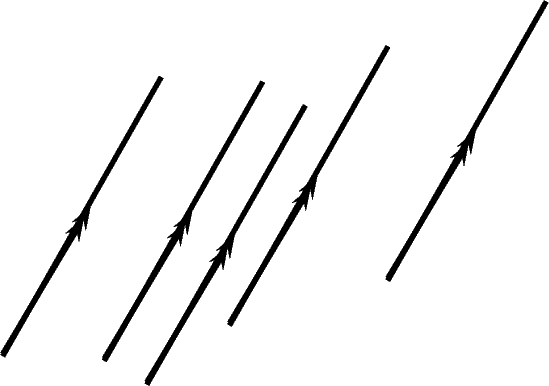
\includegraphics{col11306.imgs/m39370_MG10C13_010.png} % m39370;MG10C13\_010.png;;;6.0;8.5;
        
      \vspace{2pt}
    \vspace{.1in}
    
    \end{center}

 \end{figure}   

    \addtocounter{footnote}{-0}
    
        \par 
        \label{m39370*id316235}All these lines are parallel to each other. Notice the pair of arrow symbols for parallel.\par 
\label{m39370*notfhsst!!!underscore!!!id438}
\begin{tabular}{cc}
	\hspace*{-50pt}\raisebox{-8 mm}{\hspace{-0.2in}
\includegraphics[width=0.75in]{col11306.imgs/psfact2.png} } & 

	\begin{minipage}{0.85\textwidth}
	\begin{note}
      {note: }
        \label{m39370*id316245}A section of the Australian National Railways Trans-Australian line is perhaps one of the longest pairs of man-made parallel lines.\par 
        \label{m39370*id316258}
          \label{m39370*id316258!!!underscore!!!quote}\begin{quote}{\sl \textbf{Longest Railroad Straight} (Source: www.guinnessworldrecords.com)
The Australian National Railways Trans-Australian line over the Nullarbor Plain, is 478~km (297 miles) dead straight, from Mile 496, between Nurina and Loongana, Western Australia, to Mile 793, between Ooldea and Watson, South Australia.} % end \textsl
    \end{quote}
    
        \par 
	\end{note}
	\end{minipage}
	\end{tabular}
	\par
      
        \label{m39370*id316273}A \textsl{transversal} of two or more lines is a line that intersects these lines. For example in Figure~12.13, \begin{math}AB\end{math} and \begin{math}CD\end{math} are two parallel lines and \begin{math}EF\end{math} is a transversal. We say \begin{math}AB\parallel CD\end{math}. The properties of the angles formed by these intersecting lines are summarised in the table below.\par 
        
    \setcounter{subfigure}{0}


	\begin{figure}[H] % horizontal\label{m39370*uid29}
    \begin{center}
    \rule[.1in]{\figurerulewidth}{.005in} \\
        \label{m39370*uid29!!!underscore!!!media}\label{m39370*uid29!!!underscore!!!printimage}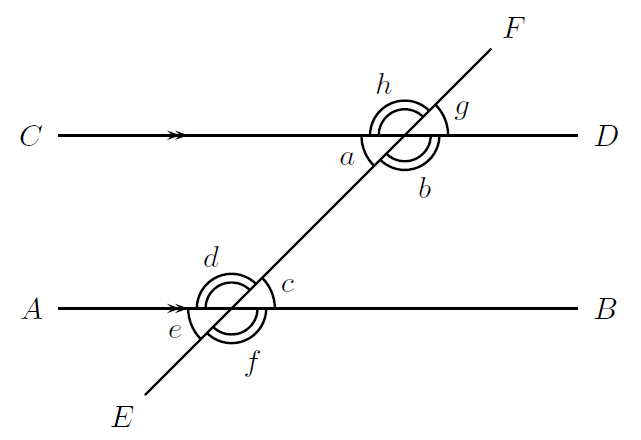
\includegraphics{col11306.imgs/m39370_MG10C13_011.png} % m39370;MG10C13\_011.png;;;6.0;8.5;
        
      \vspace{2pt}
    \vspace{\rubberspace}\par \begin{cnxcaption}
	  \small \textbf{Figure 12.13: }Parallel lines intersected by a transversal
	\end{cnxcaption}
      
    \vspace{.1in}
    \rule[.1in]{\figurerulewidth}{.005in} \\
        
    \end{center}

 \end{figure}   

    \addtocounter{footnote}{-0}
    
        
    % \textbf{m39370*uid30}\par
    
    % how many colspecs?  4
          % name: cnx:colspec
            % colnum: 1
            % colwidth: 3cm
            % latex-name: columna
            % colname: angle
            % align/tgroup-align/default: //left
            % -------------------------
            % name: cnx:colspec
            % colnum: 2
            % colwidth: 3cm
            % latex-name: columnb
            % colname: Def
            % align/tgroup-align/default: //left
            % -------------------------
            % name: cnx:colspec
            % colnum: 3
            % colwidth: 3cm
            % latex-name: columnc
            % colname: Eg
            % align/tgroup-align/default: //left
            % -------------------------
            % name: cnx:colspec
            % colnum: 4
            % colwidth: 20*
            % latex-name: columnd
            % colname: notes
            % align/tgroup-align/default: left//left
            % -------------------------
      
    
    \setlength\mytablespace{8\tabcolsep}
    \addtolength\mytablespace{5\arrayrulewidth}
    \setlength\mytablewidth{\linewidth}
        
    
    \setlength\mytableroom{\mytablewidth}
    \addtolength\mytableroom{-\mytablespace}
    
    \setlength\myfixedwidth{0pt}
        \addtolength\myfixedwidth{3cm}
    \addtolength\myfixedwidth{3cm}
    \addtolength\myfixedwidth{3cm}
\setlength\mystarwidth{\mytableroom}
        \addtolength\mystarwidth{-\myfixedwidth}
        \divide\mystarwidth 20
        
    
            % ----- Table with code
            
    % \begin{table}[H]
    % \\ '' '0'
    
        \begin{center}
      
      \label{m39370*uid30}
      
    \noindent
    \tabletail{%
        \hline
        \multicolumn{4}{|p{\mytableroom}|}{\raggedleft \small \sl continued on next page}\\
        \hline
      }
      \tablelasttail{}
      \begin{xtabular*}{\mytablewidth}[t]{|p{3cm}|p{3cm}|p{3cm}|p{20\mystarwidth}|}\hline
    % count in rowspan-info-nodeset: 4
    % align/colidx: left,1
    
    % rowcount: '0' | start: 'false' | colidx: '1'
    
        % Formatting a regular cell and recurring on the next sibling
        
                  \textbf{Name of angle}
                 &
      % align/colidx: left,2
    
    % rowcount: '0' | start: 'false' | colidx: '2'
    
        % Formatting a regular cell and recurring on the next sibling
        
                  \textbf{Definition}
                 &
      % align/colidx: left,3
    
    % rowcount: '0' | start: 'false' | colidx: '3'
    
        % Formatting a regular cell and recurring on the next sibling
        
                  \textbf{Examples}
                 &
      % align/colidx: left,4
    
    % rowcount: '0' | start: 'false' | colidx: '4'
    
        % Formatting a regular cell and recurring on the next sibling
        
                  \textbf{Notes}
                % make-rowspan-placeholders
    % rowspan info: col1 '0' | 'false' | '' || col2 '0' | 'false' | '' || col3 '0' | 'false' | '' || col4 '0' | 'false' | ''
     \tabularnewline\cline{1-1}\cline{2-2}\cline{3-3}\cline{4-4}
      %--------------------------------------------------------------------
    % align/colidx: left,1
    
    % rowcount: '0' | start: 'false' | colidx: '1'
    
        % Formatting a regular cell and recurring on the next sibling
        interior angles &
      % align/colidx: left,2
    
    % rowcount: '0' | start: 'false' | colidx: '2'
    
        % Formatting a regular cell and recurring on the next sibling
        the angles that lie inside the parallel lines &
      % align/colidx: left,3
    
    % rowcount: '0' | start: 'false' | colidx: '3'
    
        % Formatting a regular cell and recurring on the next sibling
        in Figure~12.13 \begin{math}a\end{math}, \begin{math}b\end{math}, \begin{math}c\end{math} and \begin{math}d\end{math} are interior angles &
      % align/colidx: left,4
    
    % rowcount: '0' | start: 'false' | colidx: '4'
    
        % Formatting a regular cell and recurring on the next sibling
        the word \textsl{interior} means inside% make-rowspan-placeholders
    % rowspan info: col1 '0' | 'false' | '' || col2 '0' | 'false' | '' || col3 '0' | 'false' | '' || col4 '0' | 'false' | ''
     \tabularnewline\cline{1-1}\cline{2-2}\cline{3-3}\cline{4-4}
      %--------------------------------------------------------------------
    % align/colidx: left,1
    
    % rowcount: '0' | start: 'false' | colidx: '1'
    
        % Formatting a regular cell and recurring on the next sibling
        adjacent angles &
      % align/colidx: left,2
    
    % rowcount: '0' | start: 'false' | colidx: '2'
    
        % Formatting a regular cell and recurring on the next sibling
        the angles share a common vertex point and line &
      % align/colidx: left,3
    
    % rowcount: '0' | start: 'false' | colidx: '3'
    
        % Formatting a regular cell and recurring on the next sibling
        in Figure~12.13 (\begin{math}a\end{math}, \begin{math}h\end{math}) are adjacent and so are (\begin{math}h\end{math}, \begin{math}g\end{math}); (\begin{math}g\end{math}, \begin{math}b\end{math}); (\begin{math}b\end{math}, \begin{math}a\end{math}) &
      % align/colidx: left,4
    
    % rowcount: '0' | start: 'false' | colidx: '4'
    
        % Formatting a regular cell and recurring on the next sibling
        % make-rowspan-placeholders
    % rowspan info: col1 '0' | 'false' | '' || col2 '0' | 'false' | '' || col3 '0' | 'false' | '' || col4 '0' | 'false' | ''
     \tabularnewline\cline{1-1}\cline{2-2}\cline{3-3}\cline{4-4}
      %--------------------------------------------------------------------
    % align/colidx: left,1
    
    % rowcount: '0' | start: 'false' | colidx: '1'
    
        % Formatting a regular cell and recurring on the next sibling
        exterior angles &
      % align/colidx: left,2
    
    % rowcount: '0' | start: 'false' | colidx: '2'
    
        % Formatting a regular cell and recurring on the next sibling
        the angles that lie outside the parallel lines &
      % align/colidx: left,3
    
    % rowcount: '0' | start: 'false' | colidx: '3'
    
        % Formatting a regular cell and recurring on the next sibling
        in Figure~12.13 \begin{math}e\end{math}, \begin{math}f\end{math}, \begin{math}g\end{math} and \begin{math}h\end{math} are exterior angles &
      % align/colidx: left,4
    
    % rowcount: '0' | start: 'false' | colidx: '4'
    
        % Formatting a regular cell and recurring on the next sibling
        the word \textsl{exterior} means outside% make-rowspan-placeholders
    % rowspan info: col1 '0' | 'false' | '' || col2 '0' | 'false' | '' || col3 '0' | 'false' | '' || col4 '0' | 'false' | ''
     \tabularnewline\cline{1-1}\cline{2-2}\cline{3-3}\cline{4-4}
      %--------------------------------------------------------------------
    % align/colidx: left,1
    
    % rowcount: '0' | start: 'false' | colidx: '1'
    
        % Formatting a regular cell and recurring on the next sibling
        alternate interior angles &
      % align/colidx: left,2
    
    % rowcount: '0' | start: 'false' | colidx: '2'
    
        % Formatting a regular cell and recurring on the next sibling
        the interior angles that lie on opposite sides of the transversal &
      % align/colidx: left,3
    
    % rowcount: '0' | start: 'false' | colidx: '3'
    
        % Formatting a regular cell and recurring on the next sibling
        in Figure~12.13 (\begin{math}a,c\end{math}) and (\begin{math}b\end{math},\begin{math}d\end{math}) are pairs of alternate interior angles, \begin{math}a=c\end{math}, \begin{math}b=d\end{math} &
      % align/colidx: left,4
    
    % rowcount: '0' | start: 'false' | colidx: '4'
    
        % Formatting a regular cell and recurring on the next sibling
        
                  
    \setcounter{subfigure}{0}

\label{m39370*id316794}
    \begin{center}
    \label{m39370*id316794!!!underscore!!!media}\label{m39370*id316794!!!underscore!!!printimage}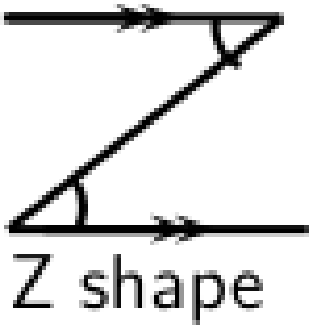
\includegraphics{col11306.imgs/m39370_MG10C13_012.png} % m39370;MG10C13\_012.png;;;6.0;8.5;
        
      \vspace{2pt}
    \vspace{.1in}
    
    \end{center}



    \addtocounter{footnote}{-0}
    
                % make-rowspan-placeholders
    % rowspan info: col1 '0' | 'false' | '' || col2 '0' | 'false' | '' || col3 '0' | 'false' | '' || col4 '0' | 'false' | ''
     \tabularnewline\cline{1-1}\cline{2-2}\cline{3-3}\cline{4-4}
      %--------------------------------------------------------------------
    % align/colidx: left,1
    
    % rowcount: '0' | start: 'false' | colidx: '1'
    
        % Formatting a regular cell and recurring on the next sibling
        co-interior angles on the same side &
      % align/colidx: left,2
    
    % rowcount: '0' | start: 'false' | colidx: '2'
    
        % Formatting a regular cell and recurring on the next sibling
        co-interior angles that lie on the same side of the transversal &
      % align/colidx: left,3
    
    % rowcount: '0' | start: 'false' | colidx: '3'
    
        % Formatting a regular cell and recurring on the next sibling
        in Figure~12.13 (\begin{math}a\end{math},\begin{math}d\end{math}) and (\begin{math}b\end{math},\begin{math}c\end{math}) are interior angles on the same side. \begin{math}a+d={180}^{\circ }\end{math}, \begin{math}b+c={180}^{\circ }\end{math} &
      % align/colidx: left,4
    
    % rowcount: '0' | start: 'false' | colidx: '4'
    
        % Formatting a regular cell and recurring on the next sibling
        
                  
    \setcounter{subfigure}{0}

\label{m39370*id316923}
    \begin{center}
    \label{m39370*id316923!!!underscore!!!media}\label{m39370*id316923!!!underscore!!!printimage}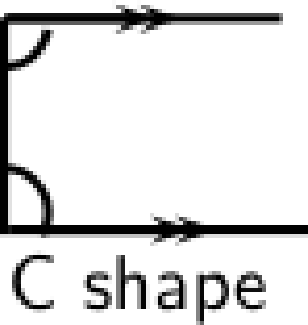
\includegraphics{col11306.imgs/m39370_MG10C13_013.png} % m39370;MG10C13\_013.png;;;6.0;8.5;
        
      \vspace{2pt}
    \vspace{.1in}
    
    \end{center}



    \addtocounter{footnote}{-0}
    
                % make-rowspan-placeholders
    % rowspan info: col1 '0' | 'false' | '' || col2 '0' | 'false' | '' || col3 '0' | 'false' | '' || col4 '0' | 'false' | ''
     \tabularnewline\cline{1-1}\cline{2-2}\cline{3-3}\cline{4-4}
      %--------------------------------------------------------------------
    % align/colidx: left,1
    
    % rowcount: '0' | start: 'false' | colidx: '1'
    
        % Formatting a regular cell and recurring on the next sibling
        corresponding angles &
      % align/colidx: left,2
    
    % rowcount: '0' | start: 'false' | colidx: '2'
    
        % Formatting a regular cell and recurring on the next sibling
        the angles on the same side of the transversal and the same side of the parallel lines &
      % align/colidx: left,3
    
    % rowcount: '0' | start: 'false' | colidx: '3'
    
        % Formatting a regular cell and recurring on the next sibling
        in Figure~12.13 \begin{math}\left(a,e\right)\end{math}, \begin{math}\left(b,f\right)\end{math}, \begin{math}\left(c,g\right)\end{math} and \begin{math}\left(d,h\right)\end{math} are pairs of corresponding angles.  \begin{math}a=e\end{math}, \begin{math}b=f\end{math}, \begin{math}c=g\end{math}, \begin{math}d=h\end{math} &
      % align/colidx: left,4
    
    % rowcount: '0' | start: 'false' | colidx: '4'
    
        % Formatting a regular cell and recurring on the next sibling
        
                  
    \setcounter{subfigure}{0}

\label{m39370*id317099}
    \begin{center}
    \label{m39370*id317099!!!underscore!!!media}\label{m39370*id317099!!!underscore!!!printimage}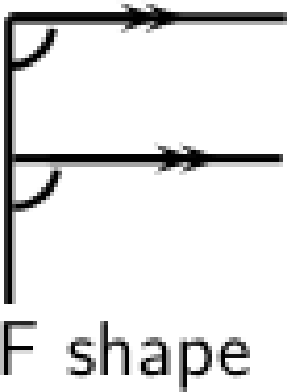
\includegraphics{col11306.imgs/m39370_MG10C13_014.png} % m39370;MG10C13\_014.png;;;6.0;8.5;
        
      \vspace{2pt}
    \vspace{.1in}
    
    \end{center}



    \addtocounter{footnote}{-0}
    
                % make-rowspan-placeholders
    % rowspan info: col1 '0' | 'false' | '' || col2 '0' | 'false' | '' || col3 '0' | 'false' | '' || col4 '0' | 'false' | ''
     \tabularnewline\cline{1-1}\cline{2-2}\cline{3-3}\cline{4-4}
      %--------------------------------------------------------------------
    \end{xtabular*}
      \end{center}
    \begin{center}{\small\bfseries Table 12.3}\end{center}
    %\end{table}
    
    \addtocounter{footnote}{-0}
    
    \par
  
\label{m39370*eip-918}The following video summarises what you have learnt so far


    \setcounter{subfigure}{0}


	\begin{figure}[H] % horizontal\label{m39370*angles-3}
    
    
    \textnormal{Khan Academy video on angles - 3}\vspace{.1in} \nopagebreak
  \label{m39370*yt-media3}\label{m39370*yt-video3}
            \raisebox{-5 pt}{ 
\includegraphics[width=0.5cm]{col11306.imgs/summary_www.png}} { (Video:  MG10090 )}
      
      \vspace{2pt}
    \vspace{.1in}
    
    

 \end{figure}   

    \addtocounter{footnote}{-0}
    \par \label{m39370*eip-933}
\begin{tabular}{cc}
	\hspace*{-50pt}\raisebox{-8 mm}{\hspace{-0.2in}
\includegraphics[width=0.75in]{col11306.imgs/psfact2.png} } & 

	\begin{minipage}{0.85\textwidth}
	\begin{note}
      {note: }\textbf{Euclid's Parallel line postulate.} If a straight line falling across two other straight lines makes the two interior angles on the same side less than two right angles (180\begin{math}{}^{\circ }\end{math}), the two straight lines, if produced indefinitely, will meet on that side.
This postulate can be used to prove many identities about the angles formed when two parallel lines are cut by a transversal. 
	\end{note}
	\end{minipage}
	\end{tabular}
	\par
      
\label{m39370*notfhsst!!!underscore!!!id534}
\begin{tabular}{cc}
	   \hspace*{-50pt}\raisebox{-8 mm}{ 
\includegraphics[width=0.5in]{col11306.imgs/pstip2.png}  }& 

	\begin{minipage}{0.85\textwidth}
	\begin{note}
      {tip: }
        \label{m39370*id317145}\begin{enumerate}[noitemsep, label=\textbf{\arabic*}. ] 
            \label{m39370*uid31}\item If two parallel lines are intersected by a transversal, the sum of the co-interior angles on the same side of the transversal is 180\begin{math}{}^{\circ }\end{math}.
\label{m39370*uid32}\item If two parallel lines are intersected by a transversal, the alternate interior angles are equal.
\label{m39370*uid33}\item If two parallel lines are intersected by a transversal, the corresponding angles are equal.
\label{m39370*uid34}\item If two lines are intersected by a transversal such that any pair of co-interior angles on the same side is supplementary, then the two lines are parallel.
\label{m39370*uid35}\item If two lines are intersected by a transversal such that a pair of alternate interior angles are equal, then the lines are parallel.
\label{m39370*uid36}\item If two lines are intersected by a transversal such that a pair of alternate corresponding angles are equal, then the lines are parallel.
\end{enumerate}
        

	\end{note}
	\end{minipage}
	\end{tabular}
	\par
      
\par
            \label{m39370*eip-499}\vspace{.5cm} 
      
      \noindent
      \hspace*{-30pt}
\includegraphics[width=0.5in]{col11306.imgs/pspencil2.png}   \raisebox{25mm}{   
      \begin{mdframed}[linewidth=4, leftmargin=40, rightmargin=40]  
      \begin{exercise}
    \noindent\textbf{Exercise 12.1: Finding angles}\label{m39370*eip-769}
  \label{m39370*eip-384}
    Find all the unknown angles in the following figure:

    \setcounter{subfigure}{0}


	\begin{figure}[H] % horizontal\label{m39370*id63478}
    \begin{center}
    \label{m39370*id63478!!!underscore!!!media}\label{m39370*id63478!!!underscore!!!printimage}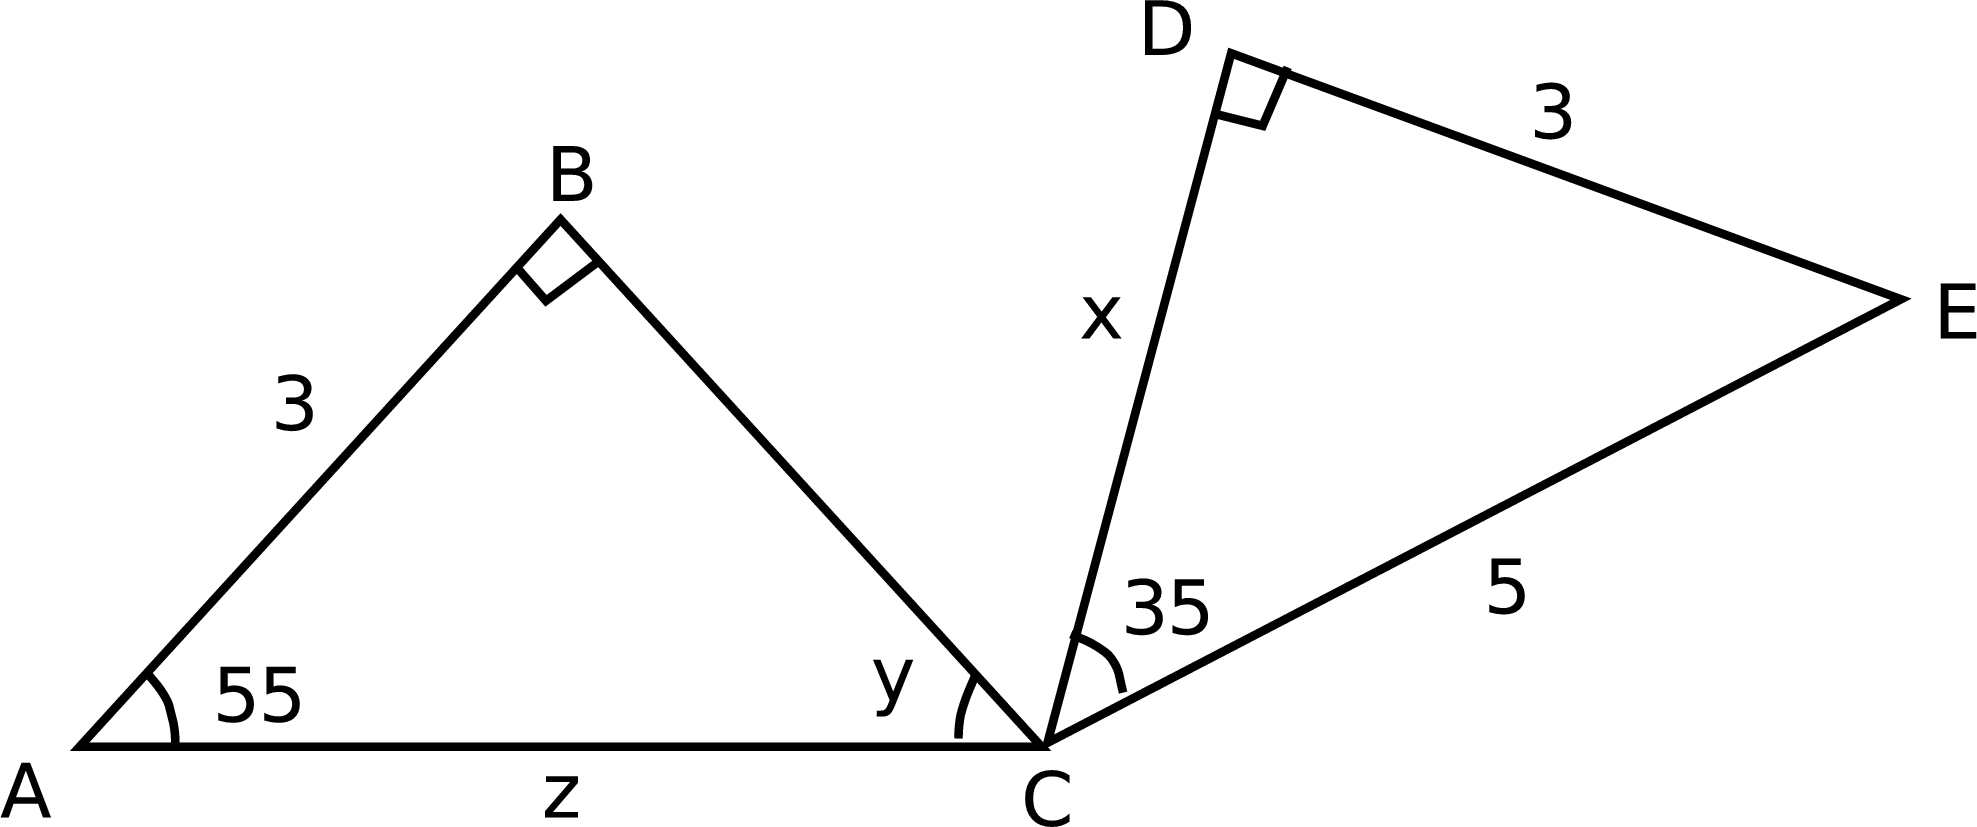
\includegraphics{col11306.imgs/m39370_angle1.png} % m39370;angle1.png;;;6.0;8.5;
        
      \vspace{2pt}
    \vspace{.1in}
    
    \end{center}

 \end{figure}   

    \addtocounter{footnote}{-0}
    
  \par 
\vspace{5pt}

\label{m39370*eip-775}\noindent\textbf{Solution to Exercise }
  \label{m39370*eip-312}\begin{enumerate}[noitemsep, label=\textbf{Step} \textbf{\arabic*}. ] 
            \leftskip=20pt\rightskip=\leftskip\item \begin{math}\text{AB}\parallel \text{CD}\end{math}. So 
\begin{math}x={30}^{\ensuremath{{\,}^{\circ}}}\end{math} (alternate interior angles)\item \label{m39370*eid6734}\nopagebreak\noindent{}\settowidth{\mymathboxwidth}{\begin{equation}
    \begin{array}{ccc}\hfill 160+y& =& 180\hfill \\ \hfill y& =& {20}^{\ensuremath{{\,}^{\circ}}}\hfill \end{array}\tag{12.1}
      \end{equation}
    }
    \typeout{Columnwidth = \the\columnwidth}\typeout{math as usual width = \the\mymathboxwidth}
    \ifthenelse{\lengthtest{\mymathboxwidth < \columnwidth}}{% if the math fits, do it again, for real
    \begin{equation}
    \begin{array}{ccc}\hfill 160+y& =& 180\hfill \\ \hfill y& =& {20}^{\ensuremath{{\,}^{\circ}}}\hfill \end{array}\tag{12.1}
      \end{equation}
    }{% else, if it doesn't fit
    \setlength{\mymathboxwidth}{\columnwidth}
      \addtolength{\mymathboxwidth}{-48pt}
    \par\vspace{12pt}\noindent\begin{minipage}{\columnwidth}
    \parbox[t]{\mymathboxwidth}{\large\begin{math}
    160+y=180y={20}^{\ensuremath{{\,}^{\circ}}}\end{math}}\hfill
    \parbox[t]{48pt}{\raggedleft 
    (12.1)}
    \end{minipage}\vspace{12pt}\par
    }% end of conditional for this bit of math
    \typeout{math as usual width = \the\mymathboxwidth}
     (co-interior angles on the same side)\end{enumerate}
        


    \end{exercise}
    \end{mdframed}
    }
    \noindent
  \par
            \label{m39370*eip-882}\vspace{.5cm} 
      
      \noindent
      \hspace*{-30pt}
\includegraphics[width=0.5in]{col11306.imgs/pspencil2.png}   \raisebox{25mm}{   
      \begin{mdframed}[linewidth=4, leftmargin=40, rightmargin=40]  
      \begin{exercise}
    \noindent\textbf{Exercise 12.2: Parallel lines}\label{m39370*eip-529}
  \label{m39370*eip-438}
    Determine if there are any parallel lines in the following figure:

    \setcounter{subfigure}{0}


	\begin{figure}[H] % horizontal\label{m39370*id9876}
    \begin{center}
    \label{m39370*id9876!!!underscore!!!media}\label{m39370*id9876!!!underscore!!!printimage}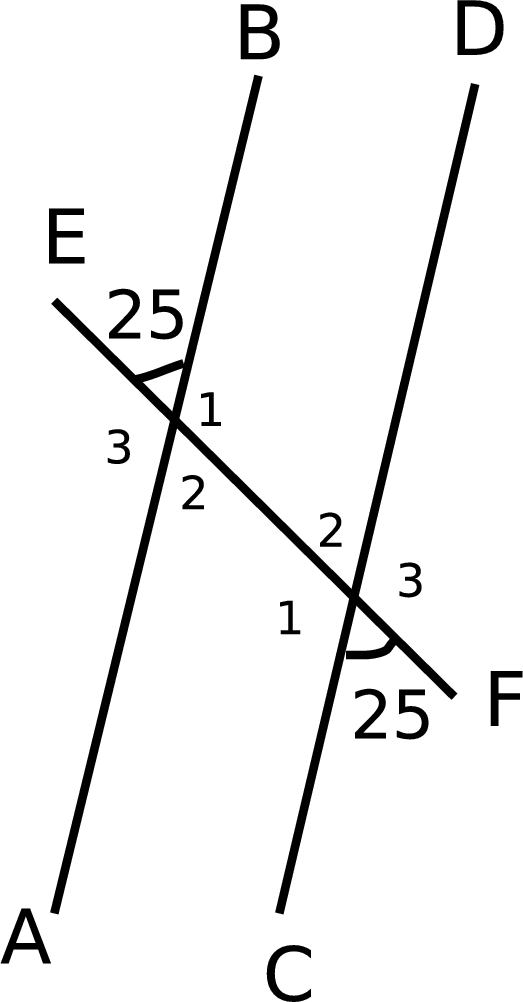
\includegraphics[height=300px]{col11306.imgs/m39370_angle2.png} % m39370;angle2.png;;;6.0;8.5;
        
      \vspace{2pt}
    \vspace{.1in}
    
    \end{center}

 \end{figure}   

    \addtocounter{footnote}{-0}
    
  \par 
\vspace{5pt}

\label{m39370*eip-668}\noindent\textbf{Solution to Exercise }
  \label{m39370*eip-82}\begin{enumerate}[noitemsep, label=\textbf{Step} \textbf{\arabic*}. ] 
            \leftskip=20pt\rightskip=\leftskip\item Line EF cannot be parallel to either AB or CD since it cuts both these lines. Lines AB and CD may be parallel.\item We can show that two lines are parallel if we can find one of the pairs of special angles. We know that 
\begin{math}{\stackrel{ˆ}{E}}_{2}={25}^{\ensuremath{{\,}^{\circ}}}\end{math}(opposite angles). And then we note that 
\label{m39370*eid6634}\nopagebreak\noindent{}\settowidth{\mymathboxwidth}{\begin{equation}
    \begin{array}{ccc}\hfill {\stackrel{ˆ}{E}}_{2}& =& {\stackrel{ˆ}{F}}_{4}\hfill \\ & =& {25}^{\ensuremath{{\,}^{\circ}}}\hfill \end{array}\tag{12.2}
      \end{equation}
    }
    \typeout{Columnwidth = \the\columnwidth}\typeout{math as usual width = \the\mymathboxwidth}
    \ifthenelse{\lengthtest{\mymathboxwidth < \columnwidth}}{% if the math fits, do it again, for real
    \begin{equation}
    \begin{array}{ccc}\hfill {\stackrel{ˆ}{E}}_{2}& =& {\stackrel{ˆ}{F}}_{4}\hfill \\ & =& {25}^{\ensuremath{{\,}^{\circ}}}\hfill \end{array}\tag{12.2}
      \end{equation}
    }{% else, if it doesn't fit
    \setlength{\mymathboxwidth}{\columnwidth}
      \addtolength{\mymathboxwidth}{-48pt}
    \par\vspace{12pt}\noindent\begin{minipage}{\columnwidth}
    \parbox[t]{\mymathboxwidth}{\large\begin{math}
    {\stackrel{ˆ}{E}}_{2}={\stackrel{ˆ}{F}}_{4}={25}^{\ensuremath{{\,}^{\circ}}}\end{math}}\hfill
    \parbox[t]{48pt}{\raggedleft 
    (12.2)}
    \end{minipage}\vspace{12pt}\par
    }% end of conditional for this bit of math
    \typeout{math as usual width = \the\mymathboxwidth}
     So we have shown that 
\begin{math}\text{AB}\parallel \text{CD}\end{math}\hspace{1ex}(corresponding angles)\end{enumerate}
        


    \end{exercise}
    \end{mdframed}
    }
    \noindent
  \label{m39370*secfhsst!!!underscore!!!id550}
            \subsubsection{ Angles }
            \nopagebreak
            \label{m39370*eip-407}\begin{enumerate}[noitemsep, label=\textbf{\arabic*}. ] 
            \item Use adjacent, corresponding, co-interior and alternate angles to fill in all the angles labeled with letters in the diagram below:

    \setcounter{subfigure}{0}


	\begin{figure}[H] % horizontal\label{m39370*id317272}
    \begin{center}
    \label{m39370*id317272!!!underscore!!!media}\label{m39370*id317272!!!underscore!!!printimage}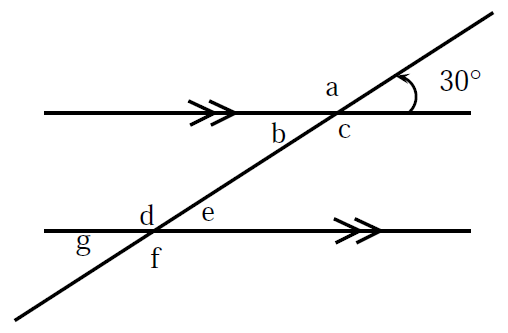
\includegraphics{col11306.imgs/m39370_MG10C13_015.png} % m39370;MG10C13\_015.png;;;6.0;8.5;
        
      \vspace{2pt}
    \vspace{.1in}
    
    \end{center}

 \end{figure}   

    \addtocounter{footnote}{-0}
            \item Find all the unknown angles in the figure below:

    \setcounter{subfigure}{0}


	\begin{figure}[H] % horizontal\label{m39370*id317298}
    \begin{center}
    \label{m39370*id317298!!!underscore!!!media}\label{m39370*id317298!!!underscore!!!printimage}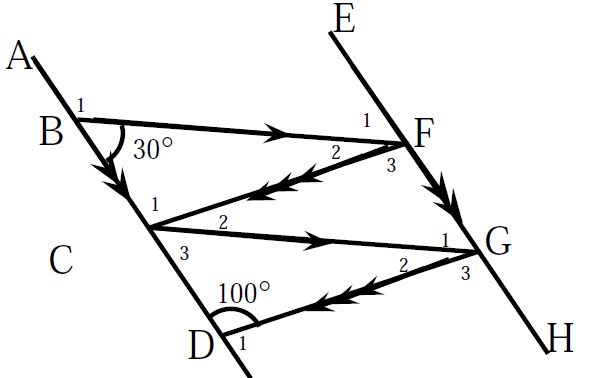
\includegraphics{col11306.imgs/m39370_MG10C13_016.png} % m39370;MG10C13\_016.png;;;6.0;8.5;
        
      \vspace{2pt}
    \vspace{.1in}
    
    \end{center}

 \end{figure}   

    \addtocounter{footnote}{-0}
            \item Find the value of \begin{math}x\end{math} in the figure below:

    \setcounter{subfigure}{0}


	\begin{figure}[H] % horizontal\label{m39370*id317330}
    \begin{center}
    \label{m39370*id317330!!!underscore!!!media}\label{m39370*id317330!!!underscore!!!printimage}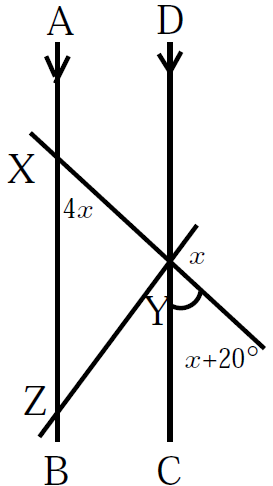
\includegraphics{col11306.imgs/m39370_MG10C13_017.png} % m39370;MG10C13\_017.png;;;6.0;8.5;
        
      \vspace{2pt}
    \vspace{.1in}
    
    \end{center}

 \end{figure}   

    \addtocounter{footnote}{-0}
            \item  Determine whether there are pairs of parallel lines in the following figures.
\label{m39370*id79123}\begin{enumerate}[noitemsep, label=\textbf{\alph*}. ] 
            \item 

    \setcounter{subfigure}{0}


	\begin{figure}[H] % horizontal\label{m39370*id317353}
    \begin{center}
    \label{m39370*id317353!!!underscore!!!media}\label{m39370*id317353!!!underscore!!!printimage}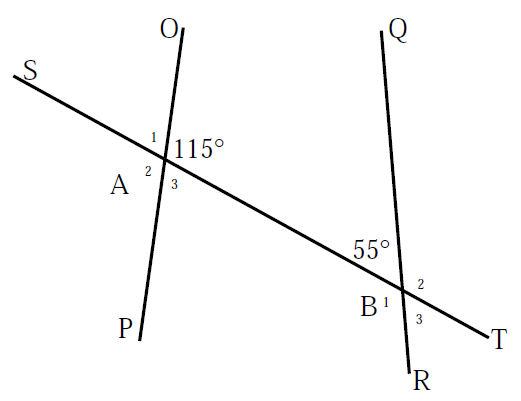
\includegraphics{col11306.imgs/m39370_MG10C13_018.png} % m39370;MG10C13\_018.png;;;6.0;8.5;
        
      \vspace{2pt}
    \vspace{.1in}
    
    \end{center}

 \end{figure}   

    \addtocounter{footnote}{-0}
    
\item 

    \setcounter{subfigure}{0}


	\begin{figure}[H] % horizontal\label{m39370*id317367}
    \begin{center}
    \label{m39370*id317367!!!underscore!!!media}\label{m39370*id317367!!!underscore!!!printimage}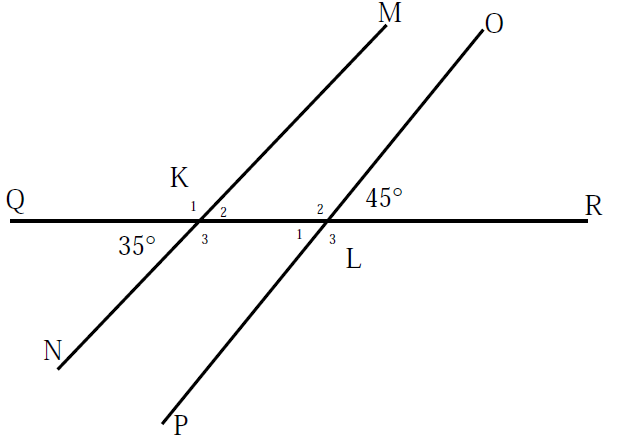
\includegraphics{col11306.imgs/m39370_MG10C13_019.png} % m39370;MG10C13\_019.png;;;6.0;8.5;
        
      \vspace{2pt}
    \vspace{.1in}
    
    \end{center}

 \end{figure}   

    \addtocounter{footnote}{-0}
    \item 

    \setcounter{subfigure}{0}


	\begin{figure}[H] % horizontal\label{m39370*id317384}
    \begin{center}
    \label{m39370*id317384!!!underscore!!!media}\label{m39370*id317384!!!underscore!!!printimage}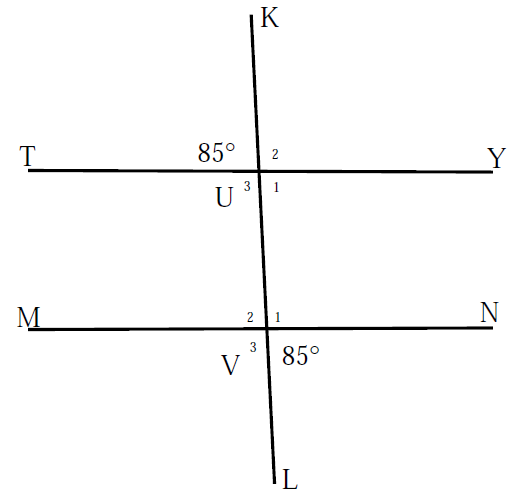
\includegraphics{col11306.imgs/m39370_MG10C13_020.png} % m39370;MG10C13\_020.png;;;6.0;8.5;
        
      \vspace{2pt}
    \vspace{.1in}
    
    \end{center}

 \end{figure}   

    \addtocounter{footnote}{-0}
    \end{enumerate}
                \item If AB is parallel to CD and AB is parallel to EF, prove that CD is parallel to EF:


    \setcounter{subfigure}{0}


	\begin{figure}[H] % horizontal\label{m39370*id317408}
    \begin{center}
    \label{m39370*id317408!!!underscore!!!media}\label{m39370*id317408!!!underscore!!!printimage}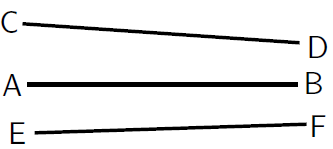
\includegraphics{col11306.imgs/m39370_MG10C13_021.png} % m39370;MG10C13\_021.png;;;6.0;8.5;
        
      \vspace{2pt}
    \vspace{.1in}
    
    \end{center}

 \end{figure}   

    \addtocounter{footnote}{-0}
            \end{enumerate}
        \label{m39370*eip-115}The following video shows some problems with their solutions


    \setcounter{subfigure}{0}


	\begin{figure}[H] % horizontal\label{m39370*angles-4}
    
    
    \textnormal{Khan Academy video on angles - 4}\vspace{.1in} \nopagebreak
  \label{m39370*yt-media4}\label{m39370*yt-video4}
            \raisebox{-5 pt}{ 
\includegraphics[width=0.5cm]{col11306.imgs/summary_www.png}} { (Video:  MG10091 )}
      
      \vspace{2pt}
    \vspace{.1in}
    
    

 \end{figure}   

    \addtocounter{footnote}{-0}
    \par 
        

      
    
  \label{m39370**end}
          
\par \raisebox{-5 pt}{
\includegraphics[width=0.5cm]{col11306.imgs/summary_www.png}} Find the answers with the shortcodes:
 \par \begin{tabular}[h]{cccccc}
 (1.) lxF  &  (2.) lxL  &  (3.) lxM  &  (4.) lxe  &  (5.) lxt  & \end{tabular}



         \section{ Polygons}
    \nopagebreak
            \label{m39368} $ \hspace{-5pt}\begin{array}{cccccccccccc}   
\includegraphics[width=0.75cm]{col11306.imgs/summary_fullmarks.png} &   \end{array} $ \hspace{2 pt}\raisebox{-5 pt}{} {(section shortcode: MG10092 )} \par 
    
    
    
    
    
    
  
    
    
    
    
    \label{m39368*cid5}
            \subsection{ Polygons}
            \nopagebreak
            
      
      \label{m39368*id317435}If you take some lines and join them such that the end point of the first line meets the starting point of the last line, you will get a \textsl{polygon}. Each line that makes up the polygon is known as a \textsl{side}. A polygon has interior angles. These are the angles that are inside the polygon. The number of sides of a polygon equals the number of interior angles. If a polygon has equal length sides and equal interior angles, then the polygon is called a \textsl{regular polygon}. Some examples of polygons are shown in Figure~12.28.\par 
      
    \setcounter{subfigure}{0}


	\begin{figure}[H] % horizontal\label{m39368*uid37}
    \begin{center}
    \rule[.1in]{\figurerulewidth}{.005in} \\
        \label{m39368*uid37!!!underscore!!!media}\label{m39368*uid37!!!underscore!!!printimage}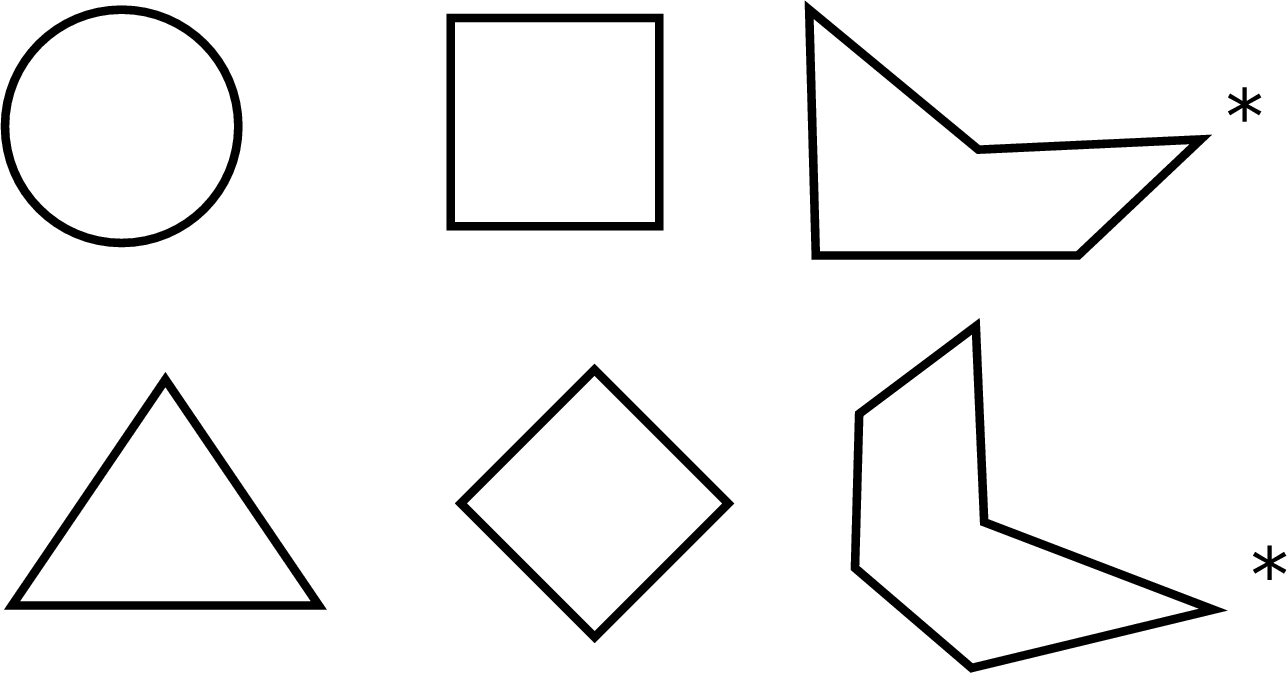
\includegraphics{col11306.imgs/m39368_MG10C13_0221.png} % m39368;MG10C13\_0221.png;;;6.0;8.5;
        
      \vspace{2pt}
    \vspace{\rubberspace}\par \begin{cnxcaption}
	  \small \textbf{Figure 12.28: }Examples of polygons. They are all regular, except for the one marked *
	\end{cnxcaption}
      
    \vspace{.1in}
    \rule[.1in]{\figurerulewidth}{.005in} \\
        
    \end{center}

 \end{figure}   

    \addtocounter{footnote}{-0}
    
      \label{m39368*uid38}
            \subsubsection{ Triangles}
            \nopagebreak
            \label{m39368*id317485}A triangle is a three-sided polygon. Triangles are usually split into three categories: equilateral, isosceles, and scalene, depending on how many of the sides are of equal length. A fourth category, right-angled triangle (or simply 'right triangle') is used to refer to triangles with one right angle. Note that all right-angled triangles are also either isosceles (if the other two sides are equal) or scalene (it should be clear why you cannot have an equilateral right triangle!). The properties of these triangles are summarised in Table 12.4.\par 
        
    % \textbf{m39368*uid39}\par
    
    % how many colspecs?  3
          % name: cnx:colspec
            % colnum: 1
            % colwidth: 10*
            % latex-name: columna
            % colname: 
            % align/tgroup-align/default: //left
            % -------------------------
            % name: cnx:colspec
            % colnum: 2
            % colwidth: 10*
            % latex-name: columnb
            % colname: 
            % align/tgroup-align/default: //left
            % -------------------------
            % name: cnx:colspec
            % colnum: 3
            % colwidth: 10*
            % latex-name: columnc
            % colname: 
            % align/tgroup-align/default: //left
            % -------------------------
      
    
    \setlength\mytablespace{6\tabcolsep}
    \addtolength\mytablespace{4\arrayrulewidth}
    \setlength\mytablewidth{\linewidth}
        
    
    \setlength\mytableroom{\mytablewidth}
    \addtolength\mytableroom{-\mytablespace}
    
    \setlength\myfixedwidth{0pt}
    \setlength\mystarwidth{\mytableroom}
        \addtolength\mystarwidth{-\myfixedwidth}
        \divide\mystarwidth 30
        
    
            % ----- Table with code
            
    % \begin{table}[H]
    % \\ '' '0'
    
        \begin{center}
      
      \label{m39368*uid39}
      
    \noindent
    \tabletail{%
        \hline
        \multicolumn{3}{|p{\mytableroom}|}{\raggedleft \small \sl continued on next page}\\
        \hline
      }
      \tablelasttail{}
      \begin{xtabular*}{\mytablewidth}[t]{|p{10\mystarwidth}|p{10\mystarwidth}|p{10\mystarwidth}|}\hline
    % count in rowspan-info-nodeset: 3
    % align/colidx: left,1
    
    % rowcount: '0' | start: 'false' | colidx: '1'
    
        % Formatting a regular cell and recurring on the next sibling
        Name &
      % align/colidx: left,2
    
    % rowcount: '0' | start: 'false' | colidx: '2'
    
        % Formatting a regular cell and recurring on the next sibling
        Diagram &
      % align/colidx: left,3
    
    % rowcount: '0' | start: 'false' | colidx: '3'
    
        % Formatting a regular cell and recurring on the next sibling
        Properties% make-rowspan-placeholders
    % rowspan info: col1 '0' | 'false' | '' || col2 '0' | 'false' | '' || col3 '0' | 'false' | ''
     \tabularnewline\cline{1-1}\cline{2-2}\cline{3-3}
      %--------------------------------------------------------------------
    % align/colidx: left,1
    
    % rowcount: '0' | start: 'false' | colidx: '1'
    
        % Formatting a regular cell and recurring on the next sibling
        equilateral &
      % align/colidx: left,2
    
    % rowcount: '0' | start: 'false' | colidx: '2'
    
        % Formatting a regular cell and recurring on the next sibling
        
                  
    \setcounter{subfigure}{0}

\label{m39368*id317558}
    \begin{center}
    \label{m39368*id317558!!!underscore!!!media}\label{m39368*id317558!!!underscore!!!printimage}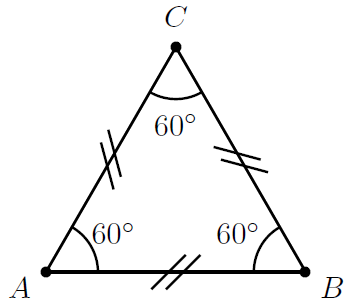
\includegraphics{col11306.imgs/m39368_MG10C13_023.png} % m39368;MG10C13\_023.png;;;6.0;8.5;
        
      \vspace{2pt}
    \vspace{.1in}
    
    \end{center}



    \addtocounter{footnote}{-0}
    
                 &
      % align/colidx: left,3
    
    % rowcount: '0' | start: 'false' | colidx: '3'
    
        % Formatting a regular cell and recurring on the next sibling
        All three sides are equal in length (denoted by the short lines drawn through all the sides of equal length) and all three angles are equal.% make-rowspan-placeholders
    % rowspan info: col1 '0' | 'false' | '' || col2 '0' | 'false' | '' || col3 '0' | 'false' | ''
     \tabularnewline\cline{1-1}\cline{2-2}\cline{3-3}
      %--------------------------------------------------------------------
    % align/colidx: left,1
    
    % rowcount: '0' | start: 'false' | colidx: '1'
    
        % Formatting a regular cell and recurring on the next sibling
        isosceles &
      % align/colidx: left,2
    
    % rowcount: '0' | start: 'false' | colidx: '2'
    
        % Formatting a regular cell and recurring on the next sibling
        
                  
    \setcounter{subfigure}{0}

\label{m39368*id317593}
    \begin{center}
    \label{m39368*id317593!!!underscore!!!media}\label{m39368*id317593!!!underscore!!!printimage}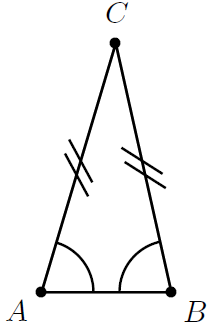
\includegraphics{col11306.imgs/m39368_MG10C13_024.png} % m39368;MG10C13\_024.png;;;6.0;8.5;
        
      \vspace{2pt}
    \vspace{.1in}
    
    \end{center}



    \addtocounter{footnote}{-0}
    
                 &
      % align/colidx: left,3
    
    % rowcount: '0' | start: 'false' | colidx: '3'
    
        % Formatting a regular cell and recurring on the next sibling
        Two sides are equal in length. The angles opposite the equal sides are equal.% make-rowspan-placeholders
    % rowspan info: col1 '0' | 'false' | '' || col2 '0' | 'false' | '' || col3 '0' | 'false' | ''
     \tabularnewline\cline{1-1}\cline{2-2}\cline{3-3}
      %--------------------------------------------------------------------
    % align/colidx: left,1
    
    % rowcount: '0' | start: 'false' | colidx: '1'
    
        % Formatting a regular cell and recurring on the next sibling
        right-angled &
      % align/colidx: left,2
    
    % rowcount: '0' | start: 'false' | colidx: '2'
    
        % Formatting a regular cell and recurring on the next sibling
        
                  
    \setcounter{subfigure}{0}

\label{m39368*id317628}
    \begin{center}
    \label{m39368*id317628!!!underscore!!!media}\label{m39368*id317628!!!underscore!!!printimage}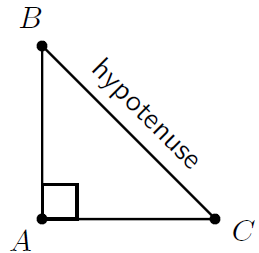
\includegraphics{col11306.imgs/m39368_MG10C13_025.png} % m39368;MG10C13\_025.png;;;6.0;8.5;
        
      \vspace{2pt}
    \vspace{.1in}
    
    \end{center}



    \addtocounter{footnote}{-0}
    
                 &
      % align/colidx: left,3
    
    % rowcount: '0' | start: 'false' | colidx: '3'
    
        % Formatting a regular cell and recurring on the next sibling
        This triangle has one right angle. The side opposite this angle is called the \textsl{hypotenuse}.% make-rowspan-placeholders
    % rowspan info: col1 '0' | 'false' | '' || col2 '0' | 'false' | '' || col3 '0' | 'false' | ''
     \tabularnewline\cline{1-1}\cline{2-2}\cline{3-3}
      %--------------------------------------------------------------------
    % align/colidx: left,1
    
    % rowcount: '0' | start: 'false' | colidx: '1'
    
        % Formatting a regular cell and recurring on the next sibling
        scalene (non-syllabus) &
      % align/colidx: left,2
    
    % rowcount: '0' | start: 'false' | colidx: '2'
    
        % Formatting a regular cell and recurring on the next sibling
        
                  
    \setcounter{subfigure}{0}

\label{m39368*id317668}
    \begin{center}
    \label{m39368*id317668!!!underscore!!!media}\label{m39368*id317668!!!underscore!!!printimage}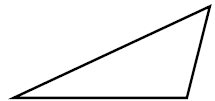
\includegraphics{col11306.imgs/m39368_MG10C13_026.png} % m39368;MG10C13\_026.png;;;6.0;8.5;
        
      \vspace{2pt}
    \vspace{.1in}
    
    \end{center}



    \addtocounter{footnote}{-0}
    
                 &
      % align/colidx: left,3
    
    % rowcount: '0' | start: 'false' | colidx: '3'
    
        % Formatting a regular cell and recurring on the next sibling
        All sides and angles are different.% make-rowspan-placeholders
    % rowspan info: col1 '0' | 'false' | '' || col2 '0' | 'false' | '' || col3 '0' | 'false' | ''
     \tabularnewline\cline{1-1}\cline{2-2}\cline{3-3}
      %--------------------------------------------------------------------
    \end{xtabular*}
      \end{center}
    \begin{center}{\small\bfseries Table 12.4}: Types of Triangles\end{center}
    %\end{table}
    
    \addtocounter{footnote}{-0}
    
    \par
  
        \label{m39368*id317683}We use the notation \begin{math}▵ABC\end{math} to refer to a triangle with corners labeled \begin{math}A\end{math}, \begin{math}B\end{math}, and \begin{math}C\end{math}.\par 
        \label{m39368*uid40}
            \subsubsection{ Properties of Triangles}
            \nopagebreak
            
          
\label{m39368*secfhsst!!!underscore!!!id655}
            \subsubsection{  Investigation : Sum of the angles in a triangle }
            \nopagebreak
            
          \label{m39368*id317720}\begin{enumerate}[noitemsep, label=\textbf{\arabic*}. ] 
            \label{m39368*uid41}\item Draw on a piece of paper a triangle of any size and shape
\label{m39368*uid42}\item Cut it out and label the angles \begin{math}\hat{A}\end{math}, \begin{math}\hat{B}\end{math} and \begin{math}\hat{C}\end{math} on both sides of the paper
\label{m39368*uid43}\item Draw dotted lines as shown and cut along these lines to get three pieces of paper
\label{m39368*uid44}\item Place them along your ruler as shown to see that \begin{math}\hat{A}+\hat{B}+\hat{C}={180}^{\circ }\end{math}\end{enumerate}
        
          \label{m39368*id317868}
    \setcounter{subfigure}{0}


	\begin{figure}[H] % horizontal\label{m39368*id317874}
    \begin{center}
    \label{m39368*id317874!!!underscore!!!media}\label{m39368*id317874!!!underscore!!!printimage}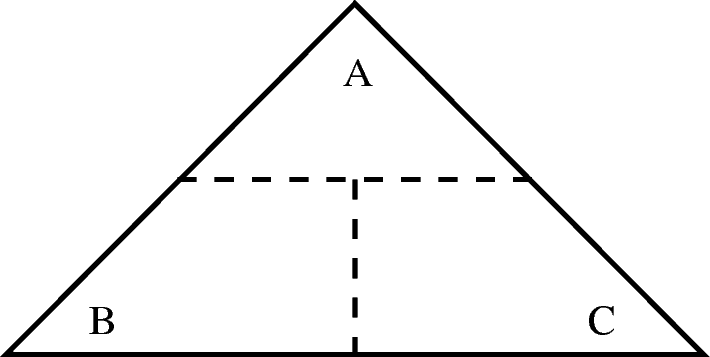
\includegraphics{col11306.imgs/m39368_MG10C13_027.png} % m39368;MG10C13\_027.png;;;6.0;8.5;
        
      \vspace{2pt}
    \vspace{.1in}
    
    \end{center}

 \end{figure}   

    \addtocounter{footnote}{-0}
    
    \setcounter{subfigure}{0}


	\begin{figure}[H] % horizontal\label{m39368*id317886}
    \begin{center}
    \label{m39368*id317886!!!underscore!!!media}\label{m39368*id317886!!!underscore!!!printimage}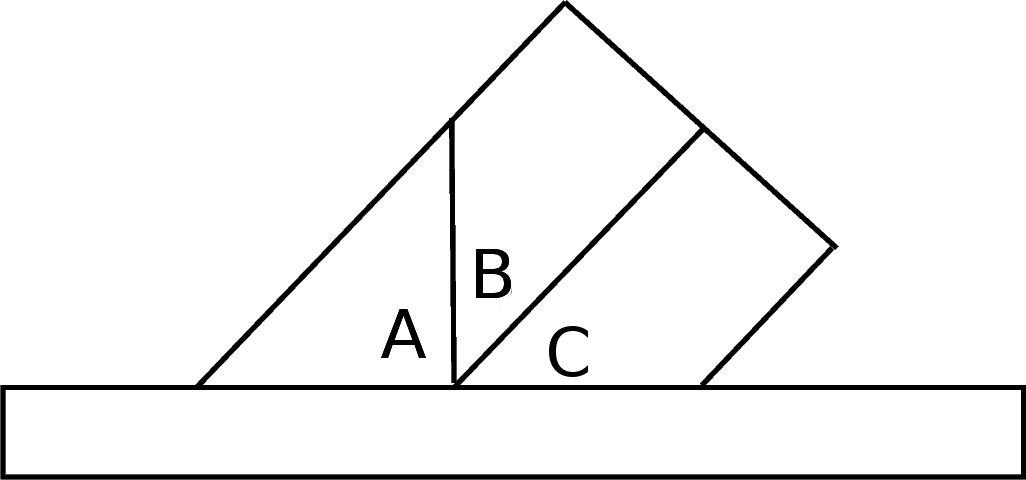
\includegraphics{col11306.imgs/m39368_MG10C13_028.png} % m39368;MG10C13\_028.png;;;6.0;8.5;
        
      \vspace{2pt}
    \vspace{.1in}
    
    \end{center}

 \end{figure}   

    \addtocounter{footnote}{-0}
    


 \par 

\label{m39368*notfhsst!!!underscore!!!id670}
\begin{tabular}{cc}
	   \hspace*{-50pt}\raisebox{-8 mm}{ 
\includegraphics[width=0.5in]{col11306.imgs/pstip2.png}  }& 

	\begin{minipage}{0.85\textwidth}
	\begin{note}
      {tip: }The sum of the angles in a triangle is 180\begin{math}{}^{\circ }\end{math}.
	\end{note}
	\end{minipage}
	\end{tabular}
	\par
      
          
    \setcounter{subfigure}{0}


	\begin{figure}[H] % horizontal\label{m39368*uid45}
    \begin{center}
    \rule[.1in]{\figurerulewidth}{.005in} \\
        \label{m39368*uid45!!!underscore!!!media}\label{m39368*uid45!!!underscore!!!printimage}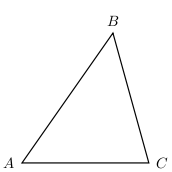
\includegraphics{col11306.imgs/m39368_MG10C13_029.png} % m39368;MG10C13\_029.png;;;6.0;8.5;
        
      \vspace{2pt}
    \vspace{\rubberspace}\par \begin{cnxcaption}
	  \small \textbf{Figure 12.35: }In any triangle, \begin{math}\angle A+\angle B+\angle C={180}^{\circ }\end{math}
	\end{cnxcaption}
      
    \vspace{.1in}
    \rule[.1in]{\figurerulewidth}{.005in} \\
        
    \end{center}

 \end{figure}   

    \addtocounter{footnote}{-0}
    
\label{m39368*notfhsst!!!underscore!!!id678}
\begin{tabular}{cc}
	   \hspace*{-50pt}\raisebox{-8 mm}{ 
\includegraphics[width=0.5in]{col11306.imgs/pstip2.png}  }& 

	\begin{minipage}{0.85\textwidth}
	\begin{note}
      {tip: }Any exterior angle of a triangle is equal to the sum of the two opposite interior angles. An exterior angle is formed by extending any one of the sides.
	\end{note}
	\end{minipage}
	\end{tabular}
	\par
      
          
    \setcounter{subfigure}{0}


	\begin{figure}[H] % horizontal\label{m39368*uid46}
    \begin{center}
    \rule[.1in]{\figurerulewidth}{.005in} \\
        \label{m39368*uid46!!!underscore!!!media}\label{m39368*uid46!!!underscore!!!printimage}\includegraphics{col11306.imgs/m39368_MG10C13_030.png} % m39368;MG10C13\_030.png;;;6.0;8.5;
        
      \vspace{2pt}
    \vspace{\rubberspace}\par \begin{cnxcaption}
	  \small \textbf{Figure 12.36: }In any triangle, any exterior angle is equal to the sum of the two opposite interior angles.
	\end{cnxcaption}
      
    \vspace{.1in}
    \rule[.1in]{\figurerulewidth}{.005in} \\
        
    \end{center}

 \end{figure}   

    \addtocounter{footnote}{-0}
    
        
        \label{m39368*uid47}
            \subsubsection{ Congruent Triangles}
            \nopagebreak
            
          
          \label{m39368*eip-370}Two triangles are called congruent if one of them can be superimposed, that is moved on top of to exactly cover, the other. In other words, if both triangles have all of the same angles and sides, then they are called congruent. To decide whether two triangles are congruent, it is not necessary to check every side and angle. The following list describes various requirements that are sufficient to know when two triangles are congruent.\par 
    % \textbf{m39368*id317997}\par
    
    % how many colspecs?  3
          % name: cnx:colspec
            % colnum: 1
            % colwidth: 10*
            % latex-name: columna
            % colname: 
            % align/tgroup-align/default: //left
            % -------------------------
            % name: cnx:colspec
            % colnum: 2
            % colwidth: 10*
            % latex-name: columnb
            % colname: 
            % align/tgroup-align/default: //left
            % -------------------------
            % name: cnx:colspec
            % colnum: 3
            % colwidth: 10*
            % latex-name: columnc
            % colname: 
            % align/tgroup-align/default: //left
            % -------------------------
      
    
    \setlength\mytablespace{6\tabcolsep}
    \addtolength\mytablespace{4\arrayrulewidth}
    \setlength\mytablewidth{\linewidth}
        
    
    \setlength\mytableroom{\mytablewidth}
    \addtolength\mytableroom{-\mytablespace}
    
    \setlength\myfixedwidth{0pt}
    \setlength\mystarwidth{\mytableroom}
        \addtolength\mystarwidth{-\myfixedwidth}
        \divide\mystarwidth 30
        
    
            % ----- Table with code
            
    % \begin{table}[H]
    % \\ '' '0'
    
        \begin{center}
      
      \label{m39368*id317997}
      
    \noindent
    \tabletail{%
        \hline
        \multicolumn{3}{|p{\mytableroom}|}{\raggedleft \small \sl continued on next page}\\
        \hline
      }
      \tablelasttail{}
      \begin{xtabular*}{\mytablewidth}[t]{|p{10\mystarwidth}|p{10\mystarwidth}|p{10\mystarwidth}|}\hline
    % count in rowspan-info-nodeset: 3
    % align/colidx: left,1
    
    % rowcount: '0' | start: 'false' | colidx: '1'
    
        % Formatting a regular cell and recurring on the next sibling
        
                    \textbf{Label}
                   &
      % align/colidx: left,2
    
    % rowcount: '0' | start: 'false' | colidx: '2'
    
        % Formatting a regular cell and recurring on the next sibling
        
                    \textbf{Description}
                   &
      % align/colidx: left,3
    
    % rowcount: '0' | start: 'false' | colidx: '3'
    
        % Formatting a regular cell and recurring on the next sibling
        
                    \textbf{Diagram}
                  % make-rowspan-placeholders
    % rowspan info: col1 '0' | 'false' | '' || col2 '0' | 'false' | '' || col3 '0' | 'false' | ''
     \tabularnewline\cline{1-1}\cline{2-2}\cline{3-3}
      %--------------------------------------------------------------------
    % align/colidx: left,1
    
    % rowcount: '0' | start: 'false' | colidx: '1'
    
        % Formatting a regular cell and recurring on the next sibling
        RHS &
      % align/colidx: left,2
    
    % rowcount: '0' | start: 'false' | colidx: '2'
    
        % Formatting a regular cell and recurring on the next sibling
        If the hypotenuse and one side of a right-angled triangle are equal to the hypotenuse and the respective side of another triangle, then the triangles are congruent. &
      % align/colidx: left,3
    
    % rowcount: '0' | start: 'false' | colidx: '3'
    
        % Formatting a regular cell and recurring on the next sibling
        
                    
    \setcounter{subfigure}{0}

\label{m39368*id318071}
    \begin{center}
    \label{m39368*id318071!!!underscore!!!media}\label{m39368*id318071!!!underscore!!!printimage}\includegraphics{col11306.imgs/m39368_MG10C13_031.png} % m39368;MG10C13\_031.png;;;6.0;8.5;
        
      \vspace{2pt}
    \vspace{.1in}
    
    \end{center}



    \addtocounter{footnote}{-0}
    
                  % make-rowspan-placeholders
    % rowspan info: col1 '0' | 'false' | '' || col2 '0' | 'false' | '' || col3 '0' | 'false' | ''
     \tabularnewline\cline{1-1}\cline{2-2}\cline{3-3}
      %--------------------------------------------------------------------
    % align/colidx: left,1
    
    % rowcount: '0' | start: 'false' | colidx: '1'
    
        % Formatting a regular cell and recurring on the next sibling
        SSS &
      % align/colidx: left,2
    
    % rowcount: '0' | start: 'false' | colidx: '2'
    
        % Formatting a regular cell and recurring on the next sibling
        If three sides of a triangle are equal in length to the same sides of another triangle, then the two triangles are congruent &
      % align/colidx: left,3
    
    % rowcount: '0' | start: 'false' | colidx: '3'
    
        % Formatting a regular cell and recurring on the next sibling
        
                    
    \setcounter{subfigure}{0}

\label{m39368*id318107}
    \begin{center}
    \label{m39368*id318107!!!underscore!!!media}\label{m39368*id318107!!!underscore!!!printimage}\includegraphics{col11306.imgs/m39368_MG10C13_032.png} % m39368;MG10C13\_032.png;;;6.0;8.5;
        
      \vspace{2pt}
    \vspace{.1in}
    
    \end{center}



    \addtocounter{footnote}{-0}
    
                  % make-rowspan-placeholders
    % rowspan info: col1 '0' | 'false' | '' || col2 '0' | 'false' | '' || col3 '0' | 'false' | ''
     \tabularnewline\cline{1-1}\cline{2-2}\cline{3-3}
      %--------------------------------------------------------------------
    % align/colidx: left,1
    
    % rowcount: '0' | start: 'false' | colidx: '1'
    
        % Formatting a regular cell and recurring on the next sibling
        SAS &
      % align/colidx: left,2
    
    % rowcount: '0' | start: 'false' | colidx: '2'
    
        % Formatting a regular cell and recurring on the next sibling
        If two sides and the included angle of one triangle are equal to the same two sides and included angle of another triangle, then the two triangles are congruent. &
      % align/colidx: left,3
    
    % rowcount: '0' | start: 'false' | colidx: '3'
    
        % Formatting a regular cell and recurring on the next sibling
        
                    
    \setcounter{subfigure}{0}

\label{m39368*id318143}
    \begin{center}
    \label{m39368*id318143!!!underscore!!!media}\label{m39368*id318143!!!underscore!!!printimage}\includegraphics{col11306.imgs/m39368_MG10C13_033.png} % m39368;MG10C13\_033.png;;;6.0;8.5;
        
      \vspace{2pt}
    \vspace{.1in}
    
    \end{center}



    \addtocounter{footnote}{-0}
    
                  % make-rowspan-placeholders
    % rowspan info: col1 '0' | 'false' | '' || col2 '0' | 'false' | '' || col3 '0' | 'false' | ''
     \tabularnewline\cline{1-1}\cline{2-2}\cline{3-3}
      %--------------------------------------------------------------------
    % align/colidx: left,1
    
    % rowcount: '0' | start: 'false' | colidx: '1'
    
        % Formatting a regular cell and recurring on the next sibling
        AAS &
      % align/colidx: left,2
    
    % rowcount: '0' | start: 'false' | colidx: '2'
    
        % Formatting a regular cell and recurring on the next sibling
        If one side and two angles of one triangle are equal to the same one side and two angles of another triangle, then the two triangles are congruent. &
      % align/colidx: left,3
    
    % rowcount: '0' | start: 'false' | colidx: '3'
    
        % Formatting a regular cell and recurring on the next sibling
        
                    
    \setcounter{subfigure}{0}

\label{m39368*id318178}
    \begin{center}
    \label{m39368*id318178!!!underscore!!!media}\label{m39368*id318178!!!underscore!!!printimage}\includegraphics{col11306.imgs/m39368_MG10C13_034.png} % m39368;MG10C13\_034.png;;;6.0;8.5;
        
      \vspace{2pt}
    \vspace{.1in}
    
    \end{center}



    \addtocounter{footnote}{-0}
    
                  % make-rowspan-placeholders
    % rowspan info: col1 '0' | 'false' | '' || col2 '0' | 'false' | '' || col3 '0' | 'false' | ''
     \tabularnewline\cline{1-1}\cline{2-2}\cline{3-3}
      %--------------------------------------------------------------------
    \end{xtabular*}
      \end{center}
    \begin{center}{\small\bfseries Table 12.5}\end{center}
    %\end{table}
    
    \addtocounter{footnote}{-0}
    
    \par
  
        
        \label{m39368*uid48}
            \subsubsection{ Similar Triangles}
            \nopagebreak
            
          
          \label{m39368*eip-665}Two triangles are called similar if it is possible to proportionally shrink or stretch one of them to a triangle congruent to the other. Congruent triangles are similar triangles, but similar triangles are only congruent if they are the same size to begin with.\par 
    % \textbf{m39368*id318196}\par
    
    % how many colspecs?  2
          % name: cnx:colspec
            % colnum: 1
            % colwidth: 10*
            % latex-name: columna
            % colname: 
            % align/tgroup-align/default: //left
            % -------------------------
            % name: cnx:colspec
            % colnum: 2
            % colwidth: 10*
            % latex-name: columnb
            % colname: 
            % align/tgroup-align/default: //left
            % -------------------------
      
    
    \setlength\mytablespace{4\tabcolsep}
    \addtolength\mytablespace{3\arrayrulewidth}
    \setlength\mytablewidth{\linewidth}
        
    
    \setlength\mytableroom{\mytablewidth}
    \addtolength\mytableroom{-\mytablespace}
    
    \setlength\myfixedwidth{0pt}
    \setlength\mystarwidth{\mytableroom}
        \addtolength\mystarwidth{-\myfixedwidth}
        \divide\mystarwidth 20
        
    
            % ----- Table with code
            
    % \begin{table}[H]
    % \\ '' '0'
    
        \begin{center}
      
      \label{m39368*id318196}
      
    \noindent
    \tabletail{%
        \hline
        \multicolumn{2}{|p{\mytableroom}|}{\raggedleft \small \sl continued on next page}\\
        \hline
      }
      \tablelasttail{}
      \begin{xtabular*}{\mytablewidth}[t]{|p{10\mystarwidth}|p{10\mystarwidth}|}\hline
    % count in rowspan-info-nodeset: 2
    % align/colidx: left,1
    
    % rowcount: '0' | start: 'false' | colidx: '1'
    
        % Formatting a regular cell and recurring on the next sibling
        
                    \textbf{Description}
                   &
      % align/colidx: left,2
    
    % rowcount: '0' | start: 'false' | colidx: '2'
    
        % Formatting a regular cell and recurring on the next sibling
        
                    \textbf{Diagram}
                  % make-rowspan-placeholders
    % rowspan info: col1 '0' | 'false' | '' || col2 '0' | 'false' | ''
     \tabularnewline\cline{1-1}\cline{2-2}
      %--------------------------------------------------------------------
    % align/colidx: left,1
    
    % rowcount: '0' | start: 'false' | colidx: '1'
    
        % Formatting a regular cell and recurring on the next sibling
        If all three pairs of corresponding angles of two triangles are equal, then the triangles are similar. &
      % align/colidx: left,2
    
    % rowcount: '0' | start: 'false' | colidx: '2'
    
        % Formatting a regular cell and recurring on the next sibling
        
                    
    \setcounter{subfigure}{0}

\label{m39368*id318251}
    \begin{center}
    \label{m39368*id318251!!!underscore!!!media}\label{m39368*id318251!!!underscore!!!printimage}\includegraphics{col11306.imgs/m39368_MG10C13_035.png} % m39368;MG10C13\_035.png;;;6.0;8.5;
        
      \vspace{2pt}
    \vspace{.1in}
    
    \end{center}



    \addtocounter{footnote}{-0}
    
                  % make-rowspan-placeholders
    % rowspan info: col1 '0' | 'false' | '' || col2 '0' | 'false' | ''
     \tabularnewline\cline{1-1}\cline{2-2}
      %--------------------------------------------------------------------
    % align/colidx: left,1
    
    % rowcount: '0' | start: 'false' | colidx: '1'
    
        % Formatting a regular cell and recurring on the next sibling
        If all pairs of corresponding sides of two triangles are in proportion, then the triangles are similar. &
      % align/colidx: left,2
    
    % rowcount: '0' | start: 'false' | colidx: '2'
    
        % Formatting a regular cell and recurring on the next sibling
        
                    
    \setcounter{subfigure}{0}

\label{m39368*id318279}
    \begin{center}
    \label{m39368*id318279!!!underscore!!!media}\label{m39368*id318279!!!underscore!!!printimage}\includegraphics{col11306.imgs/m39368_MG10C13_036.png} % m39368;MG10C13\_036.png;;;6.0;8.5;
        
      \vspace{2pt}
    \vspace{.1in}
    
    \end{center}



    \addtocounter{footnote}{-0}
    
                    \begin{math}\frac{x}{p}=\frac{y}{q}=\frac{z}{r}\end{math}
                  % make-rowspan-placeholders
    % rowspan info: col1 '0' | 'false' | '' || col2 '0' | 'false' | ''
     \tabularnewline\cline{1-1}\cline{2-2}
      %--------------------------------------------------------------------
    \end{xtabular*}
      \end{center}
    \begin{center}{\small\bfseries Table 12.6}\end{center}
    %\end{table}
    
    \addtocounter{footnote}{-0}
    
    \par
  
        
        \label{m39368*uid49}
            \subsubsection{ The theorem of Pythagoras}
            \nopagebreak
            
          
          \label{m39368*id318328}
    \setcounter{subfigure}{0}


	\begin{figure}[H] % horizontal\label{m39368*id318334}
    \begin{center}
    \label{m39368*id318334!!!underscore!!!media}\label{m39368*id318334!!!underscore!!!printimage}\includegraphics{col11306.imgs/m39368_MG10C13_037.png} % m39368;MG10C13\_037.png;;;6.0;8.5;
        
      \vspace{2pt}
    \vspace{.1in}
    
    \end{center}

 \end{figure}   

    \addtocounter{footnote}{-0}
    



If \begin{math}▵\end{math}ABC is right-angled (\begin{math}\hat{B}={90}^{\circ }\end{math}) then
\begin{math}{b}^{2}={a}^{2}+{c}^{2}\end{math}\newline
    \textbf{Converse:}
If \begin{math}{b}^{2}={a}^{2}+{c}^{2}\end{math}, then
\begin{math}▵\end{math}ABC is right-angled (\begin{math}\hat{B}={90}^{\circ }\end{math}).

\par 
\label{m39368*eip-693}\vspace{.5cm} 
      
      \noindent
      \hspace*{-30pt}\includegraphics[width=0.5in]{col11306.imgs/pspencil2.png}   \raisebox{25mm}{   
      \begin{mdframed}[linewidth=4, leftmargin=40, rightmargin=40]  
      \begin{exercise}
    \noindent\textbf{Exercise 12.3: Triangles}\label{m39368*eip-221}
  \label{m39368*eip-154}
   In the following figure, determine if the two triangles are congruent, then use the result to help you find the unknown letters.

    \setcounter{subfigure}{0}


	\begin{figure}[H] % horizontal\label{m39368*id5433}
    \begin{center}
    \label{m39368*id5433!!!underscore!!!media}\label{m39368*id5433!!!underscore!!!printimage}\includegraphics[width=300px]{col11306.imgs/m39368_triangle1.png} % m39368;triangle1.png;;;6.0;8.5;
        
      \vspace{2pt}
    \vspace{.1in}
    
    \end{center}

 \end{figure}   

    \addtocounter{footnote}{-0}
    
  \par 
\vspace{5pt}

\label{m39368*eip-477}\noindent\textbf{Solution to Exercise }
  \label{m39368*eip-156}\begin{enumerate}[noitemsep, label=\textbf{Step} \textbf{\arabic*}. ] 
            \leftskip=20pt\rightskip=\leftskip\item \label{m39368*id65234}\begin{math}D\stackrel{ˆ}{E}C=B\stackrel{ˆ}{A}C={55}^{\ensuremath{{\,}^{\circ}}}\end{math}\hspace{1ex}(angles in a triangle add up to 
\begin{math}{180}^{\ensuremath{{\,}^{\circ}}}\end{math}).\par 
      \label{m39368*id1166232344812}\begin{math}A\stackrel{ˆ}{B}C=C\stackrel{ˆ}{D}E={90}^{\ensuremath{{\,}^{\circ}}}\end{math}\hspace{1ex} (given)\par 
      \label{m39368*id1166233687055}\begin{math}\text{DE}=\text{AB}=3\end{math}\hspace{1ex} (given)\par 
      \label{m39368*id1166230595268}\nopagebreak\noindent{}
        \settowidth{\mymathboxwidth}{\begin{equation}
    \therefore \Delta \text{ABC}\equiv \Delta \text{CDE}\tag{12.3}
      \end{equation}
    }
    \typeout{Columnwidth = \the\columnwidth}\typeout{math as usual width = \the\mymathboxwidth}
    \ifthenelse{\lengthtest{\mymathboxwidth < \columnwidth}}{% if the math fits, do it again, for real
    \begin{equation}
    \therefore \Delta \text{ABC}\equiv \Delta \text{CDE}\tag{12.3}
      \end{equation}
    }{% else, if it doesn't fit
    \setlength{\mymathboxwidth}{\columnwidth}
      \addtolength{\mymathboxwidth}{-48pt}
    \par\vspace{12pt}\noindent\begin{minipage}{\columnwidth}
    \parbox[t]{\mymathboxwidth}{\large\begin{math}
    \therefore \Delta \text{ABC}\equiv \Delta \text{CDE}\end{math}}\hfill
    \parbox[t]{48pt}{\raggedleft 
    (12.3)}
    \end{minipage}\vspace{12pt}\par
    }% end of conditional for this bit of math
    \typeout{math as usual width = \the\mymathboxwidth}
    
      \item \label{m39368*id6543}We use Pythagoras to find x: 
      \label{m39368*id1166232298669}\nopagebreak\noindent{}\settowidth{\mymathboxwidth}{\begin{equation}
    \begin{array}{ccc}\hfill {\text{CE}}^{2}& =& {\text{DE}}^{2}+{\text{DC}}^{2}\hfill \\ \hfill {5}^{2}& =& {3}^{2}+{x}^{2}\hfill \\ \hfill {x}^{2}& =& 16\hfill \\ \hfill x& =& 4\hfill \end{array}\tag{12.4}
      \end{equation}
    }
    \typeout{Columnwidth = \the\columnwidth}\typeout{math as usual width = \the\mymathboxwidth}
    \ifthenelse{\lengthtest{\mymathboxwidth < \columnwidth}}{% if the math fits, do it again, for real
    \begin{equation}
    \begin{array}{ccc}\hfill {\text{CE}}^{2}& =& {\text{DE}}^{2}+{\text{DC}}^{2}\hfill \\ \hfill {5}^{2}& =& {3}^{2}+{x}^{2}\hfill \\ \hfill {x}^{2}& =& 16\hfill \\ \hfill x& =& 4\hfill \end{array}\tag{12.4}
      \end{equation}
    }{% else, if it doesn't fit
    \setlength{\mymathboxwidth}{\columnwidth}
      \addtolength{\mymathboxwidth}{-48pt}
    \par\vspace{12pt}\noindent\begin{minipage}{\columnwidth}
    \parbox[t]{\mymathboxwidth}{\large\begin{math}
    {\text{CE}}^{2}={\text{DE}}^{2}+{\text{DC}}^{2}{5}^{2}={3}^{2}+{x}^{2}{x}^{2}=16x=4\end{math}}\hfill
    \parbox[t]{48pt}{\raggedleft 
    (12.4)}
    \end{minipage}\vspace{12pt}\par
    }% end of conditional for this bit of math
    \typeout{math as usual width = \the\mymathboxwidth}
    
      \par 
      \label{m39368*id1166229837179}\begin{math}y={35}^{\ensuremath{{\,}^{\circ}}}\end{math}\hspace{1ex}(angles in a triangle)\par 
      \label{m39368*id1166228117285}\begin{math}z=5\end{math}\hspace{1ex}(congruent triangles, 
\begin{math}\text{AC}=\text{CE}\end{math})\par \end{enumerate}
        


    \end{exercise}
    \end{mdframed}
    }
    \noindent
  \label{m39368*secfhsst!!!underscore!!!id824}
            \subsubsection{  Triangles }
            \nopagebreak
            
          \label{m39368*id318528}\begin{enumerate}[noitemsep, label=\textbf{\arabic*}. ] 
            \label{m39368*uid50}\item Calculate the unknown variables in each of the following figures. All
lengths are in mm.

    \setcounter{subfigure}{0}


	\begin{figure}[H] % horizontal\label{m39368*id318548}
    \begin{center}
    \label{m39368*id318548!!!underscore!!!media}\label{m39368*id318548!!!underscore!!!printimage}\includegraphics{col11306.imgs/m39368_MG10C13_038.png} % m39368;MG10C13\_038.png;;;6.0;8.5;
        
      \vspace{2pt}
    \vspace{.1in}
    
    \end{center}

 \end{figure}   

    \addtocounter{footnote}{-0}
            \label{m39368*uid51}\item State whether or not the following pairs of triangles are congruent or not.
Give reasons for your answers. If there is not enough information to make a
descision, say why.

    \setcounter{subfigure}{0}


	\begin{figure}[H] % horizontal\label{m39368*id318571}
    \begin{center}
    \label{m39368*id318571!!!underscore!!!media}\label{m39368*id318571!!!underscore!!!printimage}\includegraphics{col11306.imgs/m39368_MG10C13_039.png} % m39368;MG10C13\_039.png;;;6.0;8.5;
        
      \vspace{2pt}
    \vspace{.1in}
    
    \end{center}

 \end{figure}   

    \addtocounter{footnote}{-0}
            \end{enumerate}
        
          

        
  
      
      \label{m39368*eip-75}
\par \raisebox{-5 pt}{\includegraphics[width=0.5cm]{col11306.imgs/summary_www.png}} Find the answers with the shortcodes:
 \par \begin{tabular}[h]{cccccc}
 (1.) lxz  &  (2.) lxu  & \end{tabular}



            \subsubsection{ Quadrilaterals}
            \nopagebreak
            \label{m39368*eip-366}
A quadrilateral is a four sided figure. There are some special quadrilaterals (trapezium, parallelogram, kite, rhombus, square, rectangle) which you will learn about in Geometry\footnote{\raggedright{}"Geometry - Grade 10 [CAPS]" <http://http://cnx.org/content/m38381/latest/>}. 
\par \label{m39368*uid91}
            \subsubsection{ Other polygons}
            \nopagebreak
            
        
        \label{m39368*id319439}There are many other polygons, some of which are given in the table below.\par 
        
    % \textbf{m39368*uid92}\par
    
    % how many colspecs?  2
          % name: cnx:colspec
            % colnum: 1
            % colwidth: 10*
            % latex-name: columna
            % colname: 
            % align/tgroup-align/default: //left
            % -------------------------
            % name: cnx:colspec
            % colnum: 2
            % colwidth: 10*
            % latex-name: columnb
            % colname: 
            % align/tgroup-align/default: //left
            % -------------------------
      
    
    \setlength\mytablespace{4\tabcolsep}
    \addtolength\mytablespace{3\arrayrulewidth}
    \setlength\mytablewidth{\linewidth}
        
    
    \setlength\mytableroom{\mytablewidth}
    \addtolength\mytableroom{-\mytablespace}
    
    \setlength\myfixedwidth{0pt}
    \setlength\mystarwidth{\mytableroom}
        \addtolength\mystarwidth{-\myfixedwidth}
        \divide\mystarwidth 20
        
    
      % ----- Begin capturing width of table in LR mode woof
      \settowidth{\mytableboxwidth}{\begin{tabular}[t]{|l|l|}\hline
    % count in rowspan-info-nodeset: 2
    % align/colidx: left,1
    
    % rowcount: '0' | start: 'false' | colidx: '1'
    
        % Formatting a regular cell and recurring on the next sibling
        Sides &
      % align/colidx: left,2
    
    % rowcount: '0' | start: 'false' | colidx: '2'
    
        % Formatting a regular cell and recurring on the next sibling
        Name% make-rowspan-placeholders
    % rowspan info: col1 '0' | 'false' | '' || col2 '0' | 'false' | ''
     \tabularnewline\cline{1-1}\cline{2-2}
      %--------------------------------------------------------------------
    % align/colidx: left,1
    
    % rowcount: '0' | start: 'false' | colidx: '1'
    
        % Formatting a regular cell and recurring on the next sibling
        5 &
      % align/colidx: left,2
    
    % rowcount: '0' | start: 'false' | colidx: '2'
    
        % Formatting a regular cell and recurring on the next sibling
        pentagon% make-rowspan-placeholders
    % rowspan info: col1 '0' | 'false' | '' || col2 '0' | 'false' | ''
     \tabularnewline\cline{1-1}\cline{2-2}
      %--------------------------------------------------------------------
    % align/colidx: left,1
    
    % rowcount: '0' | start: 'false' | colidx: '1'
    
        % Formatting a regular cell and recurring on the next sibling
        6 &
      % align/colidx: left,2
    
    % rowcount: '0' | start: 'false' | colidx: '2'
    
        % Formatting a regular cell and recurring on the next sibling
        hexagon% make-rowspan-placeholders
    % rowspan info: col1 '0' | 'false' | '' || col2 '0' | 'false' | ''
     \tabularnewline\cline{1-1}\cline{2-2}
      %--------------------------------------------------------------------
    % align/colidx: left,1
    
    % rowcount: '0' | start: 'false' | colidx: '1'
    
        % Formatting a regular cell and recurring on the next sibling
        7 &
      % align/colidx: left,2
    
    % rowcount: '0' | start: 'false' | colidx: '2'
    
        % Formatting a regular cell and recurring on the next sibling
        heptagon% make-rowspan-placeholders
    % rowspan info: col1 '0' | 'false' | '' || col2 '0' | 'false' | ''
     \tabularnewline\cline{1-1}\cline{2-2}
      %--------------------------------------------------------------------
    % align/colidx: left,1
    
    % rowcount: '0' | start: 'false' | colidx: '1'
    
        % Formatting a regular cell and recurring on the next sibling
        8 &
      % align/colidx: left,2
    
    % rowcount: '0' | start: 'false' | colidx: '2'
    
        % Formatting a regular cell and recurring on the next sibling
        octagon% make-rowspan-placeholders
    % rowspan info: col1 '0' | 'false' | '' || col2 '0' | 'false' | ''
     \tabularnewline\cline{1-1}\cline{2-2}
      %--------------------------------------------------------------------
    % align/colidx: left,1
    
    % rowcount: '0' | start: 'false' | colidx: '1'
    
        % Formatting a regular cell and recurring on the next sibling
        10 &
      % align/colidx: left,2
    
    % rowcount: '0' | start: 'false' | colidx: '2'
    
        % Formatting a regular cell and recurring on the next sibling
        decagon% make-rowspan-placeholders
    % rowspan info: col1 '0' | 'false' | '' || col2 '0' | 'false' | ''
     \tabularnewline\cline{1-1}\cline{2-2}
      %--------------------------------------------------------------------
    % align/colidx: left,1
    
    % rowcount: '0' | start: 'false' | colidx: '1'
    
        % Formatting a regular cell and recurring on the next sibling
        15 &
      % align/colidx: left,2
    
    % rowcount: '0' | start: 'false' | colidx: '2'
    
        % Formatting a regular cell and recurring on the next sibling
        pentadecagon% make-rowspan-placeholders
    % rowspan info: col1 '0' | 'false' | '' || col2 '0' | 'false' | ''
     \tabularnewline\cline{1-1}\cline{2-2}
      %--------------------------------------------------------------------
    \end{tabular}} % end mytableboxwidth set
      \addtocounter{footnote}{-0}
      
      % ----- End capturing width of table in LR mode
    
        % ----- LR or paragraph mode: must test
        % ----- Begin capturing height of table
        \settoheight{\mytableboxheight}{\begin{tabular}[t]{|l|l|}\hline
    % count in rowspan-info-nodeset: 2
    % align/colidx: left,1
    
    % rowcount: '0' | start: 'false' | colidx: '1'
    
        % Formatting a regular cell and recurring on the next sibling
        Sides &
      % align/colidx: left,2
    
    % rowcount: '0' | start: 'false' | colidx: '2'
    
        % Formatting a regular cell and recurring on the next sibling
        Name% make-rowspan-placeholders
    % rowspan info: col1 '0' | 'false' | '' || col2 '0' | 'false' | ''
     \tabularnewline\cline{1-1}\cline{2-2}
      %--------------------------------------------------------------------
    % align/colidx: left,1
    
    % rowcount: '0' | start: 'false' | colidx: '1'
    
        % Formatting a regular cell and recurring on the next sibling
        5 &
      % align/colidx: left,2
    
    % rowcount: '0' | start: 'false' | colidx: '2'
    
        % Formatting a regular cell and recurring on the next sibling
        pentagon% make-rowspan-placeholders
    % rowspan info: col1 '0' | 'false' | '' || col2 '0' | 'false' | ''
     \tabularnewline\cline{1-1}\cline{2-2}
      %--------------------------------------------------------------------
    % align/colidx: left,1
    
    % rowcount: '0' | start: 'false' | colidx: '1'
    
        % Formatting a regular cell and recurring on the next sibling
        6 &
      % align/colidx: left,2
    
    % rowcount: '0' | start: 'false' | colidx: '2'
    
        % Formatting a regular cell and recurring on the next sibling
        hexagon% make-rowspan-placeholders
    % rowspan info: col1 '0' | 'false' | '' || col2 '0' | 'false' | ''
     \tabularnewline\cline{1-1}\cline{2-2}
      %--------------------------------------------------------------------
    % align/colidx: left,1
    
    % rowcount: '0' | start: 'false' | colidx: '1'
    
        % Formatting a regular cell and recurring on the next sibling
        7 &
      % align/colidx: left,2
    
    % rowcount: '0' | start: 'false' | colidx: '2'
    
        % Formatting a regular cell and recurring on the next sibling
        heptagon% make-rowspan-placeholders
    % rowspan info: col1 '0' | 'false' | '' || col2 '0' | 'false' | ''
     \tabularnewline\cline{1-1}\cline{2-2}
      %--------------------------------------------------------------------
    % align/colidx: left,1
    
    % rowcount: '0' | start: 'false' | colidx: '1'
    
        % Formatting a regular cell and recurring on the next sibling
        8 &
      % align/colidx: left,2
    
    % rowcount: '0' | start: 'false' | colidx: '2'
    
        % Formatting a regular cell and recurring on the next sibling
        octagon% make-rowspan-placeholders
    % rowspan info: col1 '0' | 'false' | '' || col2 '0' | 'false' | ''
     \tabularnewline\cline{1-1}\cline{2-2}
      %--------------------------------------------------------------------
    % align/colidx: left,1
    
    % rowcount: '0' | start: 'false' | colidx: '1'
    
        % Formatting a regular cell and recurring on the next sibling
        10 &
      % align/colidx: left,2
    
    % rowcount: '0' | start: 'false' | colidx: '2'
    
        % Formatting a regular cell and recurring on the next sibling
        decagon% make-rowspan-placeholders
    % rowspan info: col1 '0' | 'false' | '' || col2 '0' | 'false' | ''
     \tabularnewline\cline{1-1}\cline{2-2}
      %--------------------------------------------------------------------
    % align/colidx: left,1
    
    % rowcount: '0' | start: 'false' | colidx: '1'
    
        % Formatting a regular cell and recurring on the next sibling
        15 &
      % align/colidx: left,2
    
    % rowcount: '0' | start: 'false' | colidx: '2'
    
        % Formatting a regular cell and recurring on the next sibling
        pentadecagon% make-rowspan-placeholders
    % rowspan info: col1 '0' | 'false' | '' || col2 '0' | 'false' | ''
     \tabularnewline\cline{1-1}\cline{2-2}
      %--------------------------------------------------------------------
    \end{tabular}} % end mytableboxheight set
        \settodepth{\mytableboxdepth}{\begin{tabular}[t]{|l|l|}\hline
    % count in rowspan-info-nodeset: 2
    % align/colidx: left,1
    
    % rowcount: '0' | start: 'false' | colidx: '1'
    
        % Formatting a regular cell and recurring on the next sibling
        Sides &
      % align/colidx: left,2
    
    % rowcount: '0' | start: 'false' | colidx: '2'
    
        % Formatting a regular cell and recurring on the next sibling
        Name% make-rowspan-placeholders
    % rowspan info: col1 '0' | 'false' | '' || col2 '0' | 'false' | ''
     \tabularnewline\cline{1-1}\cline{2-2}
      %--------------------------------------------------------------------
    % align/colidx: left,1
    
    % rowcount: '0' | start: 'false' | colidx: '1'
    
        % Formatting a regular cell and recurring on the next sibling
        5 &
      % align/colidx: left,2
    
    % rowcount: '0' | start: 'false' | colidx: '2'
    
        % Formatting a regular cell and recurring on the next sibling
        pentagon% make-rowspan-placeholders
    % rowspan info: col1 '0' | 'false' | '' || col2 '0' | 'false' | ''
     \tabularnewline\cline{1-1}\cline{2-2}
      %--------------------------------------------------------------------
    % align/colidx: left,1
    
    % rowcount: '0' | start: 'false' | colidx: '1'
    
        % Formatting a regular cell and recurring on the next sibling
        6 &
      % align/colidx: left,2
    
    % rowcount: '0' | start: 'false' | colidx: '2'
    
        % Formatting a regular cell and recurring on the next sibling
        hexagon% make-rowspan-placeholders
    % rowspan info: col1 '0' | 'false' | '' || col2 '0' | 'false' | ''
     \tabularnewline\cline{1-1}\cline{2-2}
      %--------------------------------------------------------------------
    % align/colidx: left,1
    
    % rowcount: '0' | start: 'false' | colidx: '1'
    
        % Formatting a regular cell and recurring on the next sibling
        7 &
      % align/colidx: left,2
    
    % rowcount: '0' | start: 'false' | colidx: '2'
    
        % Formatting a regular cell and recurring on the next sibling
        heptagon% make-rowspan-placeholders
    % rowspan info: col1 '0' | 'false' | '' || col2 '0' | 'false' | ''
     \tabularnewline\cline{1-1}\cline{2-2}
      %--------------------------------------------------------------------
    % align/colidx: left,1
    
    % rowcount: '0' | start: 'false' | colidx: '1'
    
        % Formatting a regular cell and recurring on the next sibling
        8 &
      % align/colidx: left,2
    
    % rowcount: '0' | start: 'false' | colidx: '2'
    
        % Formatting a regular cell and recurring on the next sibling
        octagon% make-rowspan-placeholders
    % rowspan info: col1 '0' | 'false' | '' || col2 '0' | 'false' | ''
     \tabularnewline\cline{1-1}\cline{2-2}
      %--------------------------------------------------------------------
    % align/colidx: left,1
    
    % rowcount: '0' | start: 'false' | colidx: '1'
    
        % Formatting a regular cell and recurring on the next sibling
        10 &
      % align/colidx: left,2
    
    % rowcount: '0' | start: 'false' | colidx: '2'
    
        % Formatting a regular cell and recurring on the next sibling
        decagon% make-rowspan-placeholders
    % rowspan info: col1 '0' | 'false' | '' || col2 '0' | 'false' | ''
     \tabularnewline\cline{1-1}\cline{2-2}
      %--------------------------------------------------------------------
    % align/colidx: left,1
    
    % rowcount: '0' | start: 'false' | colidx: '1'
    
        % Formatting a regular cell and recurring on the next sibling
        15 &
      % align/colidx: left,2
    
    % rowcount: '0' | start: 'false' | colidx: '2'
    
        % Formatting a regular cell and recurring on the next sibling
        pentadecagon% make-rowspan-placeholders
    % rowspan info: col1 '0' | 'false' | '' || col2 '0' | 'false' | ''
     \tabularnewline\cline{1-1}\cline{2-2}
      %--------------------------------------------------------------------
    \end{tabular}} % end mytableboxdepth set
        \addtolength{\mytableboxheight}{\mytableboxdepth}
        % ----- End capturing height of table
        \addtocounter{footnote}{-0}
        
        \ifthenelse{\mytableboxwidth<\textwidth}{% the table fits in LR mode
          \addtolength{\mytableboxwidth}{-\mytablespace}
          \typeout{textheight: \the\textheight}
          \typeout{mytableboxheight: \the\mytableboxheight}
          \typeout{textwidth: \the\textwidth}
          \typeout{mytableboxwidth: \the\mytableboxwidth}
          \ifthenelse{\mytableboxheight<\textheight}{%
        
    % \begin{table}[H]
    % \\ '' '0'
    
        \begin{center}
      
      \label{m39368*uid92}
      
    \noindent
    \begin{tabular}[t]{|l|l|}\hline
    % count in rowspan-info-nodeset: 2
    % align/colidx: left,1
    
    % rowcount: '0' | start: 'false' | colidx: '1'
    
        % Formatting a regular cell and recurring on the next sibling
        Sides &
      % align/colidx: left,2
    
    % rowcount: '0' | start: 'false' | colidx: '2'
    
        % Formatting a regular cell and recurring on the next sibling
        Name% make-rowspan-placeholders
    % rowspan info: col1 '0' | 'false' | '' || col2 '0' | 'false' | ''
     \tabularnewline\cline{1-1}\cline{2-2}
      %--------------------------------------------------------------------
    % align/colidx: left,1
    
    % rowcount: '0' | start: 'false' | colidx: '1'
    
        % Formatting a regular cell and recurring on the next sibling
        5 &
      % align/colidx: left,2
    
    % rowcount: '0' | start: 'false' | colidx: '2'
    
        % Formatting a regular cell and recurring on the next sibling
        pentagon% make-rowspan-placeholders
    % rowspan info: col1 '0' | 'false' | '' || col2 '0' | 'false' | ''
     \tabularnewline\cline{1-1}\cline{2-2}
      %--------------------------------------------------------------------
    % align/colidx: left,1
    
    % rowcount: '0' | start: 'false' | colidx: '1'
    
        % Formatting a regular cell and recurring on the next sibling
        6 &
      % align/colidx: left,2
    
    % rowcount: '0' | start: 'false' | colidx: '2'
    
        % Formatting a regular cell and recurring on the next sibling
        hexagon% make-rowspan-placeholders
    % rowspan info: col1 '0' | 'false' | '' || col2 '0' | 'false' | ''
     \tabularnewline\cline{1-1}\cline{2-2}
      %--------------------------------------------------------------------
    % align/colidx: left,1
    
    % rowcount: '0' | start: 'false' | colidx: '1'
    
        % Formatting a regular cell and recurring on the next sibling
        7 &
      % align/colidx: left,2
    
    % rowcount: '0' | start: 'false' | colidx: '2'
    
        % Formatting a regular cell and recurring on the next sibling
        heptagon% make-rowspan-placeholders
    % rowspan info: col1 '0' | 'false' | '' || col2 '0' | 'false' | ''
     \tabularnewline\cline{1-1}\cline{2-2}
      %--------------------------------------------------------------------
    % align/colidx: left,1
    
    % rowcount: '0' | start: 'false' | colidx: '1'
    
        % Formatting a regular cell and recurring on the next sibling
        8 &
      % align/colidx: left,2
    
    % rowcount: '0' | start: 'false' | colidx: '2'
    
        % Formatting a regular cell and recurring on the next sibling
        octagon% make-rowspan-placeholders
    % rowspan info: col1 '0' | 'false' | '' || col2 '0' | 'false' | ''
     \tabularnewline\cline{1-1}\cline{2-2}
      %--------------------------------------------------------------------
    % align/colidx: left,1
    
    % rowcount: '0' | start: 'false' | colidx: '1'
    
        % Formatting a regular cell and recurring on the next sibling
        10 &
      % align/colidx: left,2
    
    % rowcount: '0' | start: 'false' | colidx: '2'
    
        % Formatting a regular cell and recurring on the next sibling
        decagon% make-rowspan-placeholders
    % rowspan info: col1 '0' | 'false' | '' || col2 '0' | 'false' | ''
     \tabularnewline\cline{1-1}\cline{2-2}
      %--------------------------------------------------------------------
    % align/colidx: left,1
    
    % rowcount: '0' | start: 'false' | colidx: '1'
    
        % Formatting a regular cell and recurring on the next sibling
        15 &
      % align/colidx: left,2
    
    % rowcount: '0' | start: 'false' | colidx: '2'
    
        % Formatting a regular cell and recurring on the next sibling
        pentadecagon% make-rowspan-placeholders
    % rowspan info: col1 '0' | 'false' | '' || col2 '0' | 'false' | ''
     \tabularnewline\cline{1-1}\cline{2-2}
      %--------------------------------------------------------------------
    \end{tabular}
      \end{center}
    \begin{center}{\small\bfseries Table 12.7}: Table of some polygons and their number of sides.\end{center}
    %\end{table}
    
    \addtocounter{footnote}{-0}
    
          }{ % else
        
    % \begin{table}[H]
    % \\ '' '0'
    
        \begin{center}
      
      \label{m39368*uid92}
      
    \noindent
    \tabletail{%
        \hline
        \multicolumn{2}{|p{\mytableboxwidth}|}{\raggedleft \small \sl continued on next page}\\
        \hline
      }
      \tablelasttail{}
      \begin{xtabular}[t]{|l|l|}\hline
    % count in rowspan-info-nodeset: 2
    % align/colidx: left,1
    
    % rowcount: '0' | start: 'false' | colidx: '1'
    
        % Formatting a regular cell and recurring on the next sibling
        Sides &
      % align/colidx: left,2
    
    % rowcount: '0' | start: 'false' | colidx: '2'
    
        % Formatting a regular cell and recurring on the next sibling
        Name% make-rowspan-placeholders
    % rowspan info: col1 '0' | 'false' | '' || col2 '0' | 'false' | ''
     \tabularnewline\cline{1-1}\cline{2-2}
      %--------------------------------------------------------------------
    % align/colidx: left,1
    
    % rowcount: '0' | start: 'false' | colidx: '1'
    
        % Formatting a regular cell and recurring on the next sibling
        5 &
      % align/colidx: left,2
    
    % rowcount: '0' | start: 'false' | colidx: '2'
    
        % Formatting a regular cell and recurring on the next sibling
        pentagon% make-rowspan-placeholders
    % rowspan info: col1 '0' | 'false' | '' || col2 '0' | 'false' | ''
     \tabularnewline\cline{1-1}\cline{2-2}
      %--------------------------------------------------------------------
    % align/colidx: left,1
    
    % rowcount: '0' | start: 'false' | colidx: '1'
    
        % Formatting a regular cell and recurring on the next sibling
        6 &
      % align/colidx: left,2
    
    % rowcount: '0' | start: 'false' | colidx: '2'
    
        % Formatting a regular cell and recurring on the next sibling
        hexagon% make-rowspan-placeholders
    % rowspan info: col1 '0' | 'false' | '' || col2 '0' | 'false' | ''
     \tabularnewline\cline{1-1}\cline{2-2}
      %--------------------------------------------------------------------
    % align/colidx: left,1
    
    % rowcount: '0' | start: 'false' | colidx: '1'
    
        % Formatting a regular cell and recurring on the next sibling
        7 &
      % align/colidx: left,2
    
    % rowcount: '0' | start: 'false' | colidx: '2'
    
        % Formatting a regular cell and recurring on the next sibling
        heptagon% make-rowspan-placeholders
    % rowspan info: col1 '0' | 'false' | '' || col2 '0' | 'false' | ''
     \tabularnewline\cline{1-1}\cline{2-2}
      %--------------------------------------------------------------------
    % align/colidx: left,1
    
    % rowcount: '0' | start: 'false' | colidx: '1'
    
        % Formatting a regular cell and recurring on the next sibling
        8 &
      % align/colidx: left,2
    
    % rowcount: '0' | start: 'false' | colidx: '2'
    
        % Formatting a regular cell and recurring on the next sibling
        octagon% make-rowspan-placeholders
    % rowspan info: col1 '0' | 'false' | '' || col2 '0' | 'false' | ''
     \tabularnewline\cline{1-1}\cline{2-2}
      %--------------------------------------------------------------------
    % align/colidx: left,1
    
    % rowcount: '0' | start: 'false' | colidx: '1'
    
        % Formatting a regular cell and recurring on the next sibling
        10 &
      % align/colidx: left,2
    
    % rowcount: '0' | start: 'false' | colidx: '2'
    
        % Formatting a regular cell and recurring on the next sibling
        decagon% make-rowspan-placeholders
    % rowspan info: col1 '0' | 'false' | '' || col2 '0' | 'false' | ''
     \tabularnewline\cline{1-1}\cline{2-2}
      %--------------------------------------------------------------------
    % align/colidx: left,1
    
    % rowcount: '0' | start: 'false' | colidx: '1'
    
        % Formatting a regular cell and recurring on the next sibling
        15 &
      % align/colidx: left,2
    
    % rowcount: '0' | start: 'false' | colidx: '2'
    
        % Formatting a regular cell and recurring on the next sibling
        pentadecagon% make-rowspan-placeholders
    % rowspan info: col1 '0' | 'false' | '' || col2 '0' | 'false' | ''
     \tabularnewline\cline{1-1}\cline{2-2}
      %--------------------------------------------------------------------
    \end{xtabular}
      \end{center}
    \begin{center}{\small\bfseries Table 12.7}: Table of some polygons and their number of sides.\end{center}
    %\end{table}
    
    \addtocounter{footnote}{-0}
    
          } % 
        }{% else
        % typeset the table in paragraph mode
        % ----- Begin capturing height of table
        \settoheight{\mytableboxheight}{\begin{tabular*}{\mytablewidth}[t]{|p{10\mystarwidth}|p{10\mystarwidth}|}\hline
    % count in rowspan-info-nodeset: 2
    % align/colidx: left,1
    
    % rowcount: '0' | start: 'false' | colidx: '1'
    
        % Formatting a regular cell and recurring on the next sibling
        Sides &
      % align/colidx: left,2
    
    % rowcount: '0' | start: 'false' | colidx: '2'
    
        % Formatting a regular cell and recurring on the next sibling
        Name% make-rowspan-placeholders
    % rowspan info: col1 '0' | 'false' | '' || col2 '0' | 'false' | ''
     \tabularnewline\cline{1-1}\cline{2-2}
      %--------------------------------------------------------------------
    % align/colidx: left,1
    
    % rowcount: '0' | start: 'false' | colidx: '1'
    
        % Formatting a regular cell and recurring on the next sibling
        5 &
      % align/colidx: left,2
    
    % rowcount: '0' | start: 'false' | colidx: '2'
    
        % Formatting a regular cell and recurring on the next sibling
        pentagon% make-rowspan-placeholders
    % rowspan info: col1 '0' | 'false' | '' || col2 '0' | 'false' | ''
     \tabularnewline\cline{1-1}\cline{2-2}
      %--------------------------------------------------------------------
    % align/colidx: left,1
    
    % rowcount: '0' | start: 'false' | colidx: '1'
    
        % Formatting a regular cell and recurring on the next sibling
        6 &
      % align/colidx: left,2
    
    % rowcount: '0' | start: 'false' | colidx: '2'
    
        % Formatting a regular cell and recurring on the next sibling
        hexagon% make-rowspan-placeholders
    % rowspan info: col1 '0' | 'false' | '' || col2 '0' | 'false' | ''
     \tabularnewline\cline{1-1}\cline{2-2}
      %--------------------------------------------------------------------
    % align/colidx: left,1
    
    % rowcount: '0' | start: 'false' | colidx: '1'
    
        % Formatting a regular cell and recurring on the next sibling
        7 &
      % align/colidx: left,2
    
    % rowcount: '0' | start: 'false' | colidx: '2'
    
        % Formatting a regular cell and recurring on the next sibling
        heptagon% make-rowspan-placeholders
    % rowspan info: col1 '0' | 'false' | '' || col2 '0' | 'false' | ''
     \tabularnewline\cline{1-1}\cline{2-2}
      %--------------------------------------------------------------------
    % align/colidx: left,1
    
    % rowcount: '0' | start: 'false' | colidx: '1'
    
        % Formatting a regular cell and recurring on the next sibling
        8 &
      % align/colidx: left,2
    
    % rowcount: '0' | start: 'false' | colidx: '2'
    
        % Formatting a regular cell and recurring on the next sibling
        octagon% make-rowspan-placeholders
    % rowspan info: col1 '0' | 'false' | '' || col2 '0' | 'false' | ''
     \tabularnewline\cline{1-1}\cline{2-2}
      %--------------------------------------------------------------------
    % align/colidx: left,1
    
    % rowcount: '0' | start: 'false' | colidx: '1'
    
        % Formatting a regular cell and recurring on the next sibling
        10 &
      % align/colidx: left,2
    
    % rowcount: '0' | start: 'false' | colidx: '2'
    
        % Formatting a regular cell and recurring on the next sibling
        decagon% make-rowspan-placeholders
    % rowspan info: col1 '0' | 'false' | '' || col2 '0' | 'false' | ''
     \tabularnewline\cline{1-1}\cline{2-2}
      %--------------------------------------------------------------------
    % align/colidx: left,1
    
    % rowcount: '0' | start: 'false' | colidx: '1'
    
        % Formatting a regular cell and recurring on the next sibling
        15 &
      % align/colidx: left,2
    
    % rowcount: '0' | start: 'false' | colidx: '2'
    
        % Formatting a regular cell and recurring on the next sibling
        pentadecagon% make-rowspan-placeholders
    % rowspan info: col1 '0' | 'false' | '' || col2 '0' | 'false' | ''
     \tabularnewline\cline{1-1}\cline{2-2}
      %--------------------------------------------------------------------
    \end{tabular*}} % end mytableboxheight set
        \settodepth{\mytableboxdepth}{\begin{tabular*}{\mytablewidth}[t]{|p{10\mystarwidth}|p{10\mystarwidth}|}\hline
    % count in rowspan-info-nodeset: 2
    % align/colidx: left,1
    
    % rowcount: '0' | start: 'false' | colidx: '1'
    
        % Formatting a regular cell and recurring on the next sibling
        Sides &
      % align/colidx: left,2
    
    % rowcount: '0' | start: 'false' | colidx: '2'
    
        % Formatting a regular cell and recurring on the next sibling
        Name% make-rowspan-placeholders
    % rowspan info: col1 '0' | 'false' | '' || col2 '0' | 'false' | ''
     \tabularnewline\cline{1-1}\cline{2-2}
      %--------------------------------------------------------------------
    % align/colidx: left,1
    
    % rowcount: '0' | start: 'false' | colidx: '1'
    
        % Formatting a regular cell and recurring on the next sibling
        5 &
      % align/colidx: left,2
    
    % rowcount: '0' | start: 'false' | colidx: '2'
    
        % Formatting a regular cell and recurring on the next sibling
        pentagon% make-rowspan-placeholders
    % rowspan info: col1 '0' | 'false' | '' || col2 '0' | 'false' | ''
     \tabularnewline\cline{1-1}\cline{2-2}
      %--------------------------------------------------------------------
    % align/colidx: left,1
    
    % rowcount: '0' | start: 'false' | colidx: '1'
    
        % Formatting a regular cell and recurring on the next sibling
        6 &
      % align/colidx: left,2
    
    % rowcount: '0' | start: 'false' | colidx: '2'
    
        % Formatting a regular cell and recurring on the next sibling
        hexagon% make-rowspan-placeholders
    % rowspan info: col1 '0' | 'false' | '' || col2 '0' | 'false' | ''
     \tabularnewline\cline{1-1}\cline{2-2}
      %--------------------------------------------------------------------
    % align/colidx: left,1
    
    % rowcount: '0' | start: 'false' | colidx: '1'
    
        % Formatting a regular cell and recurring on the next sibling
        7 &
      % align/colidx: left,2
    
    % rowcount: '0' | start: 'false' | colidx: '2'
    
        % Formatting a regular cell and recurring on the next sibling
        heptagon% make-rowspan-placeholders
    % rowspan info: col1 '0' | 'false' | '' || col2 '0' | 'false' | ''
     \tabularnewline\cline{1-1}\cline{2-2}
      %--------------------------------------------------------------------
    % align/colidx: left,1
    
    % rowcount: '0' | start: 'false' | colidx: '1'
    
        % Formatting a regular cell and recurring on the next sibling
        8 &
      % align/colidx: left,2
    
    % rowcount: '0' | start: 'false' | colidx: '2'
    
        % Formatting a regular cell and recurring on the next sibling
        octagon% make-rowspan-placeholders
    % rowspan info: col1 '0' | 'false' | '' || col2 '0' | 'false' | ''
     \tabularnewline\cline{1-1}\cline{2-2}
      %--------------------------------------------------------------------
    % align/colidx: left,1
    
    % rowcount: '0' | start: 'false' | colidx: '1'
    
        % Formatting a regular cell and recurring on the next sibling
        10 &
      % align/colidx: left,2
    
    % rowcount: '0' | start: 'false' | colidx: '2'
    
        % Formatting a regular cell and recurring on the next sibling
        decagon% make-rowspan-placeholders
    % rowspan info: col1 '0' | 'false' | '' || col2 '0' | 'false' | ''
     \tabularnewline\cline{1-1}\cline{2-2}
      %--------------------------------------------------------------------
    % align/colidx: left,1
    
    % rowcount: '0' | start: 'false' | colidx: '1'
    
        % Formatting a regular cell and recurring on the next sibling
        15 &
      % align/colidx: left,2
    
    % rowcount: '0' | start: 'false' | colidx: '2'
    
        % Formatting a regular cell and recurring on the next sibling
        pentadecagon% make-rowspan-placeholders
    % rowspan info: col1 '0' | 'false' | '' || col2 '0' | 'false' | ''
     \tabularnewline\cline{1-1}\cline{2-2}
      %--------------------------------------------------------------------
    \end{tabular*}} % end mytableboxdepth set
        \addtolength{\mytableboxheight}{\mytableboxdepth}
        % ----- End capturing height of table
        \typeout{textheight: \the\textheight}
        \typeout{mytableboxheight: \the\mytableboxheight}
        \typeout{table too wide, outputting in para mode}
        
    % \begin{table}[H]
    % \\ '' '0'
    
        \begin{center}
      
      \label{m39368*uid92}
      
    \noindent
    \tabletail{%
        \hline
        \multicolumn{2}{|p{\mytableroom}|}{\raggedleft \small \sl continued on next page}\\
        \hline
      }
      \tablelasttail{}
      \begin{xtabular*}{\mytablewidth}[t]{|p{10\mystarwidth}|p{10\mystarwidth}|}\hline
    % count in rowspan-info-nodeset: 2
    % align/colidx: left,1
    
    % rowcount: '0' | start: 'false' | colidx: '1'
    
        % Formatting a regular cell and recurring on the next sibling
        Sides &
      % align/colidx: left,2
    
    % rowcount: '0' | start: 'false' | colidx: '2'
    
        % Formatting a regular cell and recurring on the next sibling
        Name% make-rowspan-placeholders
    % rowspan info: col1 '0' | 'false' | '' || col2 '0' | 'false' | ''
     \tabularnewline\cline{1-1}\cline{2-2}
      %--------------------------------------------------------------------
    % align/colidx: left,1
    
    % rowcount: '0' | start: 'false' | colidx: '1'
    
        % Formatting a regular cell and recurring on the next sibling
        5 &
      % align/colidx: left,2
    
    % rowcount: '0' | start: 'false' | colidx: '2'
    
        % Formatting a regular cell and recurring on the next sibling
        pentagon% make-rowspan-placeholders
    % rowspan info: col1 '0' | 'false' | '' || col2 '0' | 'false' | ''
     \tabularnewline\cline{1-1}\cline{2-2}
      %--------------------------------------------------------------------
    % align/colidx: left,1
    
    % rowcount: '0' | start: 'false' | colidx: '1'
    
        % Formatting a regular cell and recurring on the next sibling
        6 &
      % align/colidx: left,2
    
    % rowcount: '0' | start: 'false' | colidx: '2'
    
        % Formatting a regular cell and recurring on the next sibling
        hexagon% make-rowspan-placeholders
    % rowspan info: col1 '0' | 'false' | '' || col2 '0' | 'false' | ''
     \tabularnewline\cline{1-1}\cline{2-2}
      %--------------------------------------------------------------------
    % align/colidx: left,1
    
    % rowcount: '0' | start: 'false' | colidx: '1'
    
        % Formatting a regular cell and recurring on the next sibling
        7 &
      % align/colidx: left,2
    
    % rowcount: '0' | start: 'false' | colidx: '2'
    
        % Formatting a regular cell and recurring on the next sibling
        heptagon% make-rowspan-placeholders
    % rowspan info: col1 '0' | 'false' | '' || col2 '0' | 'false' | ''
     \tabularnewline\cline{1-1}\cline{2-2}
      %--------------------------------------------------------------------
    % align/colidx: left,1
    
    % rowcount: '0' | start: 'false' | colidx: '1'
    
        % Formatting a regular cell and recurring on the next sibling
        8 &
      % align/colidx: left,2
    
    % rowcount: '0' | start: 'false' | colidx: '2'
    
        % Formatting a regular cell and recurring on the next sibling
        octagon% make-rowspan-placeholders
    % rowspan info: col1 '0' | 'false' | '' || col2 '0' | 'false' | ''
     \tabularnewline\cline{1-1}\cline{2-2}
      %--------------------------------------------------------------------
    % align/colidx: left,1
    
    % rowcount: '0' | start: 'false' | colidx: '1'
    
        % Formatting a regular cell and recurring on the next sibling
        10 &
      % align/colidx: left,2
    
    % rowcount: '0' | start: 'false' | colidx: '2'
    
        % Formatting a regular cell and recurring on the next sibling
        decagon% make-rowspan-placeholders
    % rowspan info: col1 '0' | 'false' | '' || col2 '0' | 'false' | ''
     \tabularnewline\cline{1-1}\cline{2-2}
      %--------------------------------------------------------------------
    % align/colidx: left,1
    
    % rowcount: '0' | start: 'false' | colidx: '1'
    
        % Formatting a regular cell and recurring on the next sibling
        15 &
      % align/colidx: left,2
    
    % rowcount: '0' | start: 'false' | colidx: '2'
    
        % Formatting a regular cell and recurring on the next sibling
        pentadecagon% make-rowspan-placeholders
    % rowspan info: col1 '0' | 'false' | '' || col2 '0' | 'false' | ''
     \tabularnewline\cline{1-1}\cline{2-2}
      %--------------------------------------------------------------------
    \end{xtabular*}
      \end{center}
    \begin{center}{\small\bfseries Table 12.7}: Table of some polygons and their number of sides.\end{center}
    %\end{table}
    
    \addtocounter{footnote}{-0}
    
        }% ending lr/para test clause
      
    \par
  
        
    \setcounter{subfigure}{0}


	\begin{figure}[H] % horizontal\label{m39368*uid93}
    \begin{center}
    \rule[.1in]{\figurerulewidth}{.005in} \\
        \label{m39368*uid93!!!underscore!!!media}\label{m39368*uid93!!!underscore!!!printimage}\includegraphics{col11306.imgs/m39368_MG10C13_046.png} % m39368;MG10C13\_046.png;;;6.0;8.5;
        
      \vspace{2pt}
    \vspace{\rubberspace}\par \begin{cnxcaption}
	  \small \textbf{Figure 12.47: }Examples of other polygons.
	\end{cnxcaption}
      
    \vspace{.1in}
    \rule[.1in]{\figurerulewidth}{.005in} \\
        
    \end{center}

 \end{figure}   

    \addtocounter{footnote}{-0}
    
      \label{m39368*eip-210}
            \subsubsection{ Angles of Regular Polygons}
            \nopagebreak
            \label{m39368*id319627}Polygons need not have all sides the same. When they do, they are called regular polygons. You can calculate the size of the interior angle of a regular polygon by using:\par 
          \label{m39368*uid96}\nopagebreak\noindent{}
            \settowidth{\mymathboxwidth}{\begin{equation}
    \hat{A}=\frac{n-2}{n}\ensuremath{\times}{180}^{\circ }\tag{12.5}
      \end{equation}
    }
    \typeout{Columnwidth = \the\columnwidth}\typeout{math as usual width = \the\mymathboxwidth}
    \ifthenelse{\lengthtest{\mymathboxwidth < \columnwidth}}{% if the math fits, do it again, for real
    \begin{equation}
    \hat{A}=\frac{n-2}{n}\ensuremath{\times}{180}^{\circ }\tag{12.5}
      \end{equation}
    }{% else, if it doesn't fit
    \setlength{\mymathboxwidth}{\columnwidth}
      \addtolength{\mymathboxwidth}{-48pt}
    \par\vspace{12pt}\noindent\begin{minipage}{\columnwidth}
    \parbox[t]{\mymathboxwidth}{\large\begin{math}
    \hat{A}=\frac{n-2}{n}\ensuremath{\times}{180}^{\circ }\end{math}}\hfill
    \parbox[t]{48pt}{\raggedleft 
    (12.5)}
    \end{minipage}\vspace{12pt}\par
    }% end of conditional for this bit of math
    \typeout{math as usual width = \the\mymathboxwidth}
    
          
          \label{m39368*id319678}where \begin{math}n\end{math} is the number of sides and \begin{math}\hat{A}\end{math} is any angle.\par \label{m39368*eip-804}\vspace{.5cm} 
      
      \noindent
      \hspace*{-30pt}\includegraphics[width=0.5in]{col11306.imgs/pspencil2.png}   \raisebox{25mm}{   
      \begin{mdframed}[linewidth=4, leftmargin=40, rightmargin=40]  
      \begin{exercise}
    \noindent\textbf{Exercise 12.4}\label{m39368*eip-708}
  \label{m39368*eip-618}
    Find the size of the interior angles of a regular octagon.
  \par 
\vspace{5pt}

\label{m39368*eip-937}\noindent\textbf{Solution to Exercise }
\label{m39368*id7432}\begin{enumerate}[noitemsep, label=\textbf{Step} \textbf{\arabic*}. ] 
            \leftskip=20pt\rightskip=\leftskip\item 
An octagon has 8 sides.
\item 
\label{m39368*id7344}\nopagebreak\noindent{}
\settowidth{\mymathboxwidth}{\begin{equation}
    \begin{array}{ccc}\hfill \hat{A}& =& \frac{n-2}{n}\ensuremath{\times}{180}^{\circ }\hfill \\ \hfill \hat{A}& =& \frac{8-2}{8}\ensuremath{\times}{180}^{\circ }\hfill \\ \hfill \hat{A}& =& \frac{6}{2}\ensuremath{\times}{180}^{\circ }\hfill \\ \hfill \hat{A}& =& {135}^{\circ }\hfill \end{array}\tag{12.6}
      \end{equation}
    }
    \typeout{Columnwidth = \the\columnwidth}\typeout{math as usual width = \the\mymathboxwidth}
    \ifthenelse{\lengthtest{\mymathboxwidth < \columnwidth}}{% if the math fits, do it again, for real
    \begin{equation}
    \begin{array}{ccc}\hfill \hat{A}& =& \frac{n-2}{n}\ensuremath{\times}{180}^{\circ }\hfill \\ \hfill \hat{A}& =& \frac{8-2}{8}\ensuremath{\times}{180}^{\circ }\hfill \\ \hfill \hat{A}& =& \frac{6}{2}\ensuremath{\times}{180}^{\circ }\hfill \\ \hfill \hat{A}& =& {135}^{\circ }\hfill \end{array}\tag{12.6}
      \end{equation}
    }{% else, if it doesn't fit
    \setlength{\mymathboxwidth}{\columnwidth}
      \addtolength{\mymathboxwidth}{-48pt}
    \par\vspace{12pt}\noindent\begin{minipage}{\columnwidth}
    \parbox[t]{\mymathboxwidth}{\large\begin{math}
    \hat{A}=\frac{n-2}{n}\ensuremath{\times}{180}^{\circ }\hat{A}=\frac{8-2}{8}\ensuremath{\times}{180}^{\circ }\hat{A}=\frac{6}{2}\ensuremath{\times}{180}^{\circ }\hat{A}={135}^{\circ }\end{math}}\hfill
    \parbox[t]{48pt}{\raggedleft 
    (12.6)}
    \end{minipage}\vspace{12pt}\par
    }% end of conditional for this bit of math
    \typeout{math as usual width = \the\mymathboxwidth}
    

\end{enumerate}
        


    \end{exercise}
    \end{mdframed}
    }
    \noindent
  
       
    \label{m39368*eip-514}
            \subsection{ Summary}
            \nopagebreak
            \label{m39368*eip-439}\begin{itemize}[noitemsep]
            \item Make sure you know what the following terms mean: quadrilaterals, vertices, sides, angles, parallel lines, perpendicular lines,diagonals, bisectors and transversals.\item The properties of triangles has been covered.\item Congruency and similarity of triangles\item Angles can be classified as acute, right, obtuse, straight, reflex or revolution\item Theorem of Pythagoras which is used to calculate the lengths of sides of a right-angled triangle\item Angles: \label{m39368*id98732}\begin{itemize}[noitemsep]
            \item Acute angle: An angle \begin{math}{0}^{\circ }\end{math} and \begin{math}{90}^{\circ }\end{math}\item Right angle: An angle measuring \begin{math}{90}^{\circ }\end{math}\item Obtuse angle: An angle \begin{math}{90}^{\circ }\end{math} and \begin{math}{180}^{\circ }\end{math}\item Straight angle: An angle measuring \begin{math}{180}^{\circ }\end{math}\item Reflex angle: An angle \begin{math}{180}^{\circ }\end{math} and \begin{math}{360}^{\circ }\end{math}\item Revolution: An angle measuring \begin{math}{360}^{\circ }\end{math}\end{itemize}
        \item There are several properties of angles and some special names for these\item There are four types of triangles: Equilateral, isoceles, right-angled and scalene\item The angles in a triangle add up to \begin{math}{180}^{\circ }\end{math}\end{itemize}
        \label{m39368*cid6}
            \subsection{ Exercises}
            \nopagebreak
            \label{m39368*id320135}\begin{enumerate}[noitemsep, label=\textbf{\arabic*}. ] 
            \label{m39368*uid112}\item Find all the pairs of parallel lines in the following figures, giving reasons in each case.

\label{m39368*eip-78}\begin{enumerate}[noitemsep, label=\textbf{\alph*}. ] 
            \label{m39368*uid113}\item 
          
    \setcounter{subfigure}{0}


	\begin{figure}[H] % horizontal\label{m39368*id320164}
    \begin{center}
    \label{m39368*id320164!!!underscore!!!media}\label{m39368*id320164!!!underscore!!!printimage}\includegraphics{col11306.imgs/m39368_MG10C13_054.png} % m39368;MG10C13\_054.png;;;6.0;8.5;
        
      \vspace{2pt}
    \vspace{.1in}
    
    \end{center}

 \end{figure}   

    \addtocounter{footnote}{-0}
    
        \label{m39368*uid114}\item 
          
    \setcounter{subfigure}{0}


	\begin{figure}[H] % horizontal\label{m39368*id320183}
    \begin{center}
    \label{m39368*id320183!!!underscore!!!media}\label{m39368*id320183!!!underscore!!!printimage}\includegraphics{col11306.imgs/m39368_MG10C13_055.png} % m39368;MG10C13\_055.png;;;6.0;8.5;
        
      \vspace{2pt}
    \vspace{.1in}
    
    \end{center}

 \end{figure}   

    \addtocounter{footnote}{-0}
    
        \label{m39368*uid115}\item 
          
    \setcounter{subfigure}{0}


	\begin{figure}[H] % horizontal\label{m39368*id320201}
    \begin{center}
    \label{m39368*id320201!!!underscore!!!media}\label{m39368*id320201!!!underscore!!!printimage}\includegraphics{col11306.imgs/m39368_MG10C13_056.png} % m39368;MG10C13\_056.png;;;6.0;8.5;
        
      \vspace{2pt}
    \vspace{.1in}
    
    \end{center}

 \end{figure}   

    \addtocounter{footnote}{-0}
    
        \end{enumerate}
        
        \label{m39368*uid116}\item Find angles \begin{math}a\end{math}, \begin{math}b\end{math}, \begin{math}c\end{math} and \begin{math}d\end{math} in each case, giving reasons.
\label{m39368*id320255}\begin{enumerate}[noitemsep, label=\textbf{\alph*}. ] 
            \label{m39368*uid117}\item 
    \setcounter{subfigure}{0}


	\begin{figure}[H] % horizontal\label{m39368*id320271}
    \begin{center}
    \label{m39368*id320271!!!underscore!!!media}\label{m39368*id320271!!!underscore!!!printimage}\includegraphics{col11306.imgs/m39368_MG10C13_057.png} % m39368;MG10C13\_057.png;;;6.0;8.5;
        
      \vspace{2pt}
    \vspace{.1in}
    
    \end{center}

 \end{figure}   

    \addtocounter{footnote}{-0}
    \label{m39368*uid118}\item 
    \setcounter{subfigure}{0}


	\begin{figure}[H] % horizontal\label{m39368*id320290}
    \begin{center}
    \label{m39368*id320290!!!underscore!!!media}\label{m39368*id320290!!!underscore!!!printimage}\includegraphics{col11306.imgs/m39368_MG10C13_058.png} % m39368;MG10C13\_058.png;;;6.0;8.5;
        
      \vspace{2pt}
    \vspace{.1in}
    
    \end{center}

 \end{figure}   

    \addtocounter{footnote}{-0}
    \label{m39368*uid119}\item 
    \setcounter{subfigure}{0}


	\begin{figure}[H] % horizontal\label{m39368*id320310}
    \begin{center}
    \label{m39368*id320310!!!underscore!!!media}\label{m39368*id320310!!!underscore!!!printimage}\includegraphics{col11306.imgs/m39368_MG10C13_059.png} % m39368;MG10C13\_059.png;;;6.0;8.5;
        
      \vspace{2pt}
    \vspace{.1in}
    
    \end{center}

 \end{figure}   

    \addtocounter{footnote}{-0}
    \end{enumerate}
        
        
\label{m39368*uid126}\item Say which of the following pairs of triangles are congruent with reasons.
\label{m39368*id320498}\begin{enumerate}[noitemsep, label=\textbf{\alph*}. ] 
            \label{m39368*uid127}\item 
    \setcounter{subfigure}{0}


	\begin{figure}[H] % horizontal\label{m39368*id320512}
    \begin{center}
    \label{m39368*id320512!!!underscore!!!media}\label{m39368*id320512!!!underscore!!!printimage}\includegraphics{col11306.imgs/m39368_MG10C13_060.png} % m39368;MG10C13\_060.png;;;6.0;8.5;
        
      \vspace{2pt}
    \vspace{.1in}
    
    \end{center}

 \end{figure}   

    \addtocounter{footnote}{-0}
    \label{m39368*uid128}\item 
    \setcounter{subfigure}{0}


	\begin{figure}[H] % horizontal\label{m39368*id320530}
    \begin{center}
    \label{m39368*id320530!!!underscore!!!media}\label{m39368*id320530!!!underscore!!!printimage}\includegraphics{col11306.imgs/m39368_MG10C13_061.png} % m39368;MG10C13\_061.png;;;6.0;8.5;
        
      \vspace{2pt}
    \vspace{.1in}
    
    \end{center}

 \end{figure}   

    \addtocounter{footnote}{-0}
    \label{m39368*uid129}\item 
    \setcounter{subfigure}{0}


	\begin{figure}[H] % horizontal\label{m39368*id320548}
    \begin{center}
    \label{m39368*id320548!!!underscore!!!media}\label{m39368*id320548!!!underscore!!!printimage}\includegraphics{col11306.imgs/m39368_MG10C13_062.png} % m39368;MG10C13\_062.png;;;6.0;8.5;
        
      \vspace{2pt}
    \vspace{.1in}
    
    \end{center}

 \end{figure}   

    \addtocounter{footnote}{-0}
    \label{m39368*uid130}\item 
    \setcounter{subfigure}{0}


	\begin{figure}[H] % horizontal\label{m39368*id320565}
    \begin{center}
    \label{m39368*id320565!!!underscore!!!media}\label{m39368*id320565!!!underscore!!!printimage}\includegraphics{col11306.imgs/m39368_MG10C13_063.png} % m39368;MG10C13\_063.png;;;6.0;8.5;
        
      \vspace{2pt}
    \vspace{.1in}
    
    \end{center}

 \end{figure}   

    \addtocounter{footnote}{-0}
    \end{enumerate}
        

        \label{m39368*uid131}\item Identify the types of angles shown below (e.g. acute/obtuse etc):

          
    \setcounter{subfigure}{0}


	\begin{figure}[H] % horizontal\label{m39368*id401231}
    \begin{center}
    \label{m39368*id401231!!!underscore!!!media}\label{m39368*id401231!!!underscore!!!printimage}\includegraphics[width=300px]{col11306.imgs/m39368_MG10C13_066.png} % m39368;MG10C13\_066.png;;;6.0;8.5;
        
      \vspace{2pt}
    \vspace{.1in}
    
    \end{center}

 \end{figure}   

    \addtocounter{footnote}{-0}
    
        
\label{m39368*uid140}\item Calculate the size of the third angle (x) in each of the diagrams below:

          
    \setcounter{subfigure}{0}


	\begin{figure}[H] % horizontal\label{m39368*id401232}
    \begin{center}
    \label{m39368*id401232!!!underscore!!!media}\label{m39368*id401232!!!underscore!!!printimage}\includegraphics[width=300px]{col11306.imgs/m39368_MG10C13_067.png} % m39368;MG10C13\_067.png;;;6.0;8.5;
        
      \vspace{2pt}
    \vspace{.1in}
    
    \end{center}

 \end{figure}   

    \addtocounter{footnote}{-0}
    
        
\label{m39368*uid141}\item Name each of the shapes/polygons, state how many sides each has and whether it is regular (equiangular and equilateral) or not:

          
    \setcounter{subfigure}{0}


	\begin{figure}[H] % horizontal\label{m39368*id401233}
    \begin{center}
    \label{m39368*id401233!!!underscore!!!media}\label{m39368*id401233!!!underscore!!!printimage}\includegraphics[width=300px]{col11306.imgs/m39368_MG10C13_068.png} % m39368;MG10C13\_068.png;;;6.0;8.5;
        
      \vspace{2pt}
    \vspace{.1in}
    
    \end{center}

 \end{figure}   

    \addtocounter{footnote}{-0}
    
        
\label{m39368*uid142}\item Assess whether the following statements are true or false. If the statement is false, explain why:
\label{m39368*id401234}\begin{enumerate}[noitemsep, label=\textbf{\alph*}. ] 
            \item An angle is formed when two straight lines meet at a point.	\item The smallest angle that can be drawn is 5\ensuremath{{\,}^{\circ}}.\item An angle of 90\ensuremath{{\,}^{\circ}} is called a square angle.\item Two angles whose sum is 180\ensuremath{{\,}^{\circ}} are called supplementary angles.\item Two parallel lines will never intersect.\item A regular polygon has equal angles but not equal sides.\item An isoceles triangle has three equal sides.\item If three sides of a triangle are equal in length to the same sides of another triangle, then the two triangles are incongruent.\item If three pairs of corresponding angles in two triangles are equal, then the triangles are similar.\end{enumerate}
        
        
\label{m39368*uid143}\item Name the type of angle (e.g. acute/obtuse etc) based on it's size:
\label{m39368*id401235}\begin{enumerate}[noitemsep, label=\textbf{\alph*}. ] 
            \item  30\ensuremath{{\,}^{\circ}}\item  47\ensuremath{{\,}^{\circ}}\item  90\ensuremath{{\,}^{\circ}}\item  91\ensuremath{{\,}^{\circ}}\item  191\ensuremath{{\,}^{\circ}}\item  360\ensuremath{{\,}^{\circ}}\item  180\ensuremath{{\,}^{\circ}}\end{enumerate}
        
        
\label{m39368*uid144}\item Using Pythagoras' theorem for right-angled triangles, calculate the length of x:

          
    \setcounter{subfigure}{0}


	\begin{figure}[H] % horizontal\label{m39368*id401236}
    \begin{center}
    \label{m39368*id401236!!!underscore!!!media}\label{m39368*id401236!!!underscore!!!printimage}\includegraphics[width=300px]{col11306.imgs/m39368_MG10C13_070.png} % m39368;MG10C13\_070.png;;;6.0;8.5;
        
      \vspace{2pt}
    \vspace{.1in}
    
    \end{center}

 \end{figure}   

    \addtocounter{footnote}{-0}
    
        
\end{enumerate}
        
      \label{m39368*uid132}
\par \raisebox{-5 pt}{\includegraphics[width=0.5cm]{col11306.imgs/summary_www.png}} Find the answers with the shortcodes:
 \par \begin{tabular}[h]{cccccc}
 (1.) lxh  &  (2.) laq  &  (3.) lai  &  (4.) lTb  &  (5.) lTj  &  (6.) lTD  &  (7.) lTZ  &  (8.) lTB  &  (9.) lTK  & \end{tabular}



            \subsubsection{ Challenge Problem}
            \nopagebreak
            
        
        \label{m39368*id320611}\begin{enumerate}[noitemsep, label=\textbf{\arabic*}. ] 
            \label{m39368*uid133}\item Using the figure below, show that the sum of the three angles in a triangle is 180\begin{math}{}^{\circ }\end{math}. Line \begin{math}DE\end{math}\hspace{1ex} is parallel to \begin{math}BC\end{math}.

    \setcounter{subfigure}{0}


	\begin{figure}[H] % horizontal\label{m39368*id320668}
    \begin{center}
    \label{m39368*id320668!!!underscore!!!media}\label{m39368*id320668!!!underscore!!!printimage}\includegraphics{col11306.imgs/m39368_MG10C13_065.png} % m39368;MG10C13\_065.png;;;6.0;8.5;
        
      \vspace{2pt}
    \vspace{.1in}
    
    \end{center}

 \end{figure}   

    \addtocounter{footnote}{-0}
    \newline
            \end{enumerate}
        
      
    
  \label{m39368**end}
          
       
    
  \label{8eb3a75df362978731c03bbeab266515**end}
    
\par \raisebox{-5 pt}{\includegraphics[width=0.5cm]{col11306.imgs/summary_www.png}} Find the answers with the shortcodes:
 \par \begin{tabular}[h]{cccccc}
 (1.) laO  & \end{tabular}



